%
% Modified version of the sample_ndthesis.tex
% by Sameer Vijay
% Last Change: Wed Jul 27 2005 14:00 CEST
%
%%%%%%%%%%%%%%%%%%%%%%%%%%%%%%%%%%%%%%%%%%%%%%%%%%%%%%%%%%%%%%%%%%%%%%%%
%
% Sample Notre Dame Thesis/Dissertation
% Using Donald Peterson's ndthesis classfile
%
% Written by Jeff Squyres and Don Peterson
%
% Provided by the Information Technology Committee of
%   the Graduate Student Union
%   http://www.gsu.nd.edu/
%
% Nothing in this document is serious except the format.  :-)
%
%%%%%%%%%%%%%%%%%%%%%%%%%%%%%%%%%%%%%%%%%%%%%%%%%%%%%%%%%%%%%%%%%%%%%%%%
% This is *not* a substitute for Donald's orginial documentation.  See
% /afs/nd.edu/usr/local/src/tex/texmf/doc/latex/ndthesis/ndthesis.dvi
% for documentation on the particular commands and whatnot.
%%%%%%%%%%%%%%%%%%%%%%%%%%%%%%%%%%%%%%%%%%%%%%%%%%%%%%%%%%%%%%%%%%%%%%%%
%
% You should *also* have a ND formatting guide to ensure that you have
% all the relevant parts, put the captions in the right place, etc.
% Just because you have this wonderful style classfile doesn't mean
% that it removes *all* the formatting onus from you.  :-)
%
% Normally, you should break all of this stuff up into separate files
% (at the very least, one chapter per file) and use the \input
% command.  This is all one file for brevity's (and clarity's) sake.
%
% Note that you should also have a good Makefile; one that invokes
% LaTeX as many times as necessary (up to 4) and bibtex if necessary.
% One should be included in this distribution.  You may want to modify
% the Makefile to make separate chapters, if necessary.
%
% If you have any suggestions, comments, questions, please send e-mail
% to: ndthesis@gsu.nd.edu
%
%%%%%%%%%%%%%%%%%%%%%%%%%%%%%%%%%%%%%%%%%%%%%%%%%%%%%%%%%%%%%%%%%%%%%%%%

\documentclass[textrefs,review]{nddiss2e}

% % uncomment the following line 
% if using chapter-wise bibliography
% \usepackage{chapterbib}
% \renewcommand{\bibname}{Cited Works}
% \renewcommand{\bibsection}{\section{\bibname}}
\usepackage{algorithm}
\usepackage{algorithmic}
\usepackage{multirow}
\begin{document}

\frontmatter

\title{Potential of Opportunistic Relaying\\ {\small\scshape Performance study across wireless interfaces on smartphones} }
\author{Shu Liu}
\work{Dissertation}
\degprior{B.S., M.S.}
\degaward{Doctor of Philosophy\\in\\Computer Science and Engineering}
\advisor{Aaron Striegel}
% \secondadvisor{Gordon Gray}
\department{Computer Science and Engineering}

\maketitle
%%%%%%%%%%%%%%%%%%%%%%%%%%%%%%%%%%%%%%%%%%%%%%%%%%%%%%%%%%%%%%%%%%%%%%%%
%
% Front stuff
%
%%%%%%%%%%%%%%%%%%%%%%%%%%%%%%%%%%%%%%%%%%%%%%%%%%%%%%%%%%%%%%%%%%%%%%%%

\copyrightholder{Shu Liu}
\copyrightyear{2014}
\makecopyright

\begin{abstract}
\end{abstract}

\renewcommand{\dedicationname}{}

\begin{dedication}
  To my husband Wei
  
  and my loving parents
  
  who inspires me to exceed my potential.
   
\end{dedication}

\tableofcontents
\listoffigures
\listoftables

\begin{acknowledge}
I would like to thank my advisor, Dr. Aaron Striegel, who helped provide
direction and guidance for this work. Without his trust and support, I would not have had the opportunity to work in such great research projects. I would also like to thank the members of my committee, Dr. Christian Poellabauer, Dr. David Hachen and Dr. Gregory Madey, who were more than generous with their expertise and precious time.

I also need to thank all my colleagues who create such a good atmosphere in the group;
Andrew Blaich, Yingxin Jiang, Dirk Van Bruggen, Lei Meng, Xueheng Hu, Benjamin Bockdtege, and Rachael Purta.  Also Margaret, Tylor and Michael, deserve a special thanks because their great help in the Netsense project. I need to further thank all my dear friends, Nikhil, Hongsheng, Chris, Pramita, Sal, Jun, Yihua and Mehrdad, for being there for me throughout the entire doctorate program. 
\end{acknowledge}

\mainmatter

%
% Chapter 1
%

%
% Modified by Sameer Vijay
% Last Change: Tue Jul 26 2005 13:00 CEST
%
%%%%%%%%%%%%%%%%%%%%%%%%%%%%%%%%%%%%%%%%%%%%%%%%%%%%%%%%%%%%%%%%%%%%%%%%
%
% Sample Notre Dame Thesis/Dissertation
% Using Donald Peterson's ndthesis classfile
%
% Written by Jeff Squyres and Don Peterson
%
% Provided by the Information Technology Committee of
%   the Graduate Student Union
%   http://www.gsu.nd.edu/
%
% Nothing in this document is serious except the format.  :-)
%
% If you have any suggestions, comments, questions, please send e-mail
% to: ndthesis@gsu.nd.edu
%
%%%%%%%%%%%%%%%%%%%%%%%%%%%%%%%%%%%%%%%%%%%%%%%%%%%%%%%%%%%%%%%%%%%%%%%%


%
% Chapter 1
%

\chapter{INTRODUCTION}

\section{Overview}

Over the past few years, a vast array of wireless devices and services have emerged that are fundamentally transforming how we as a society gather and react to information.  Furthermore, the new wireless ecosystem has increased wireless data consumption at phenomenal rates with the most popular cited estimates slating traffic to double every year for the next five years \cite{CiscoAnnualCellGrowth}.  Dubbed the \emph{wireless data tsunami}, the dominant question for wireless service providers (carriers) is how to meet what appears to be an insatiable need for wireless data.  Unlike wired networks, spectrum available for wireless data is finite and typically entails massive costs for acquisition and infrastructure deployment.  Although
technologies such as LTE herald the arrival of fourth-generation (4G) wireless technology, the new speeds often only temporarily satiate the need for additional bandwidth. A wide variety of solutions have emerged ranging simpler solutions such as better WiFi offloading to much more complex solutions such as small heterogeneous cellular networks. For many cellular providers, WiFi offloading, i.e. the users receiving data from 802.11-based hotspots, offers a significant appeal by reducing the strain on the already overloaded cellular infrastructure. Recent studies such as the one in \cite{lee2010mobile} points to offloading offering gains approaching 65\% of the total traffic volume. There are other works such as \cite{balasubramanian2010augmenting, dimatteo2011cellular, han2011mobile, icc2012performance} that discuss the feasibility of WiFi offloading. 

A rich category of work that is complementary to existing techniques is the concept of \emph{opportunistic communication}. Opportunistic communication refers to the concept which allows nodes to leverage sporadic, intermittent contacts when two nodes come into direct radio communication range~\cite{pelusi2006opportunistic}. When cellular or WiFi links are not available or not strong enough, opportunistic relaying introduces another alternative option for mobile device to get connected by working in tandem with one or more devices.  From a conceptual standpoint for opportunistic networking, the design of the relaying protocol is critical, namely how does one select and manage appropriate relaying nodes as relays~\cite{laneman2004cooperative,sendonaris2003user,bletsas2006simple,lu2009design,bahl2009opportunistic}.  

The primary goal of my work is to gather high quality smartphone data and leverage the data for reinforcing analysis from a technical network system perspective with respect to network connectivity and performance enhancement. In particular, I asked three interrelated questions: \emph{(i) Can existing wireless technologies on smartphone provide accurate face-to-face proximity estimation and to what extent are relationship formation and maintenance dynamics modified with the introduction of digital communication? (ii) Can the WiFi offloading be the ultimate solution for the predicted wireless data tsunami? (iii) Can the peer-to-peer communication between mobile devices in close proximity be a good candidate for offloading cellular systems?} The answers to these questions are fascinating to explore. The NetSense project is a study of first-year students tracked over a two-year period with respect to nearly all the smartphone information. The process of gathering data results in a rich pool of digital data which provides us the opportunities to analyze the technical dynamics of the network. These involve for instance, the wireless signal strengths can reflect the relative distance and connection status. Moreover, by collecting the information of traffic consumed by the phones, we are able to compare different types of traffic usage and understand their impacts on campus wireless networks. 

\section{Contributions}
The key contributions of my dissertation is as follows:
\begin{itemize}
\item Smartphone monitoring system: By collecting data on Android smartphones, we get a fully anonymized dataset containing device information and digital communication data of participants. It is the foundation of the research and provides multiple dimensions of data for research in both network science and sociology. 

\item Bluetooth proximity: Under the premise that Bluetooth has better accuracy for short distance without the constrain of environment, we use Bluetooth signal strength as an indicator for relative distance between devices. In order to get accurate estimation of face-to-face distance, a proximity estimation model is proposed by leveraging the raw Bluetooth Received Signal Strength Indicator (RSSI) values and introducing multiple thresholds for different environments. 

\item WiFi offloading: For most cellular providers, WiFi offloading appeals to reduce the strain on the overloaded cellular infrastructure. However, based on our data, the WiFi traffic takes approximately 30\% of the total data consumption which is much lower than expected. We analyze the possible reasons for this as well as the usage patterns of users in different categorization according to their WiFi traffic consumption. 

\item Proximity relay: 
With the support of peer-to-peer communication in smartphones, it is practical to leverage the device-to-device data transfers to bridge the coverage gap between cellular and WiFi infrastructure network. Based on our data, we will do the quantitative analysis of the potential relaying which is a key missing part in relaying related research and evaluate the benefits of relaying for cellular traffic offloading in real life. 
\end{itemize}

The rest of this paper is organized as follows. Section~\ref{sec:related_work} provides an overview of the related work and Section~\ref{sec:dataset} introduces the dataset we have. Based on the dataset, the framework to evaluate the potential for relaying is proposed in Section~\ref{sec:potential}. In the end, Section~\ref{sec:conclusion} concludes the paper.



%
% Chapter 2
%

%
% Modified by Sameer Vijay
% Last Change: Wed Jul 27 2005 13:00 CEST
%
%%%%%%%%%%%%%%%%%%%%%%%%%%%%%%%%%%%%%%%%%%%%%%%%%%%%%%%%%%%%%%%%%%%%%%%%
%
% Sample Notre Dame Thesis/Dissertation
% Using Donald Peterson's ndthesis classfile
%
% Written by Jeff Squyres and Don Peterson
%
% Provided by the Information Technology Committee of
%   the Graduate Student Union
%   http://www.gsu.nd.edu/
%
% Nothing in this document is serious except the format.  :-)
%
% If you have any suggestions, comments, questions, please send e-mail
% to: ndthesis@gsu.nd.edu
%
%%%%%%%%%%%%%%%%%%%%%%%%%%%%%%%%%%%%%%%%%%%%%%%%%%%%%%%%%%%%%%%%%%%%%%%%

%
% Chapter 2
%

\chapter{Large-scale Dataset}
\label{chap:dataset}
As espoused by the MIT Reality Mining group in \cite{Nathan3,Nathan1}, the increasing availability and reliability of smartphones affords incredible opportunities for the unobtrusive gathering of data with regards to usage, location, and performance.  Although quite expensive to gather versus user self-reporting or user volunteers, a fully instrumented smartphone represents a veritable wealth of data that can afford unique insight into the smartphone performance study.

In August of 2011, two hundred participants were selected from the incoming freshmen class of our university and received a free Android smartphone and plan in exchange for agreement to participate in the two-year data collection project.  Each Android device was rooted and a custom ROM installed (Cyanogenmod) to enable the device being permanently Bluetooth discoverable. A user-level agent was installed on each of the smartphones that extracted a wide variety of environmental and usage data from the phone at periodic intervals.  The monitoring agent was installed to start automatically when the smart phone power was turned on and ran passively in the background. Tuning was conducted on the agent to ensure that even with WiFi enabled and Bluetooth always discoverable for a battery life potential at distribution of roughly one and a half days.  

\section{Data Collection}
In order to build a flexible and stable platform for delivering on-going subject queries in a secure and efficient way, we designed and implemented the monitoring system in the Fall of 2010 and did a few serials of tests before the study began. The key part of the monitoring system is the customized agent installed on the smartphones named \textit{PhoneMonitor} as illustrated in Figure~\ref{fig:agent}. The Android platform was selected for its customization capabilities through normal API or rooted/customized interfaces with respect to hardware-level interactions. It collects a variety of types of data as illustrated in table~\ref{table:data} and each kind of data is invoked through the corresponding function calls. Separate threads are employed to compensate for the variety of speeds at which the respective functions retrieve relevant data. For example, the Bluetooth data includes the detailed values of timestamp, RSSI (Received signal strength indication), MAC address, and Bluetooth identifier (BTID) with a default sensing granularity of once per minutes. The wireless environmental data (primarily WiFi) has similar fields except the access point (AP) name is recorded and the granularity of sensing is three minutes. Traffic data includes breakdowns by application and wireless adapter (cell, WiFi) with respect to both downlink (Rx) and uplink (Tx) usage at intervals down to as low as once per minute. The light sensor data, which includes the timestamp and sensor values, can help us to determine whether the phone is sheltered (e.g. inside a backpack or in hand) and the surroundings (e.g. inside or outside buildings) during the daytime. It is recorded if the current value changes more than 30 compared with the last recorded value. For mail data, both sender and receiver email addresses are recorded without content snooping. More detailed information about collected data can be found in table~\ref{table:detailed_data}. Graphic User Interface (GUI) of the application allows participants to read the last check-in time as well as the status of the network connection and Bluetooth. 

\begin{figure}[h!tbp]
\centering 
{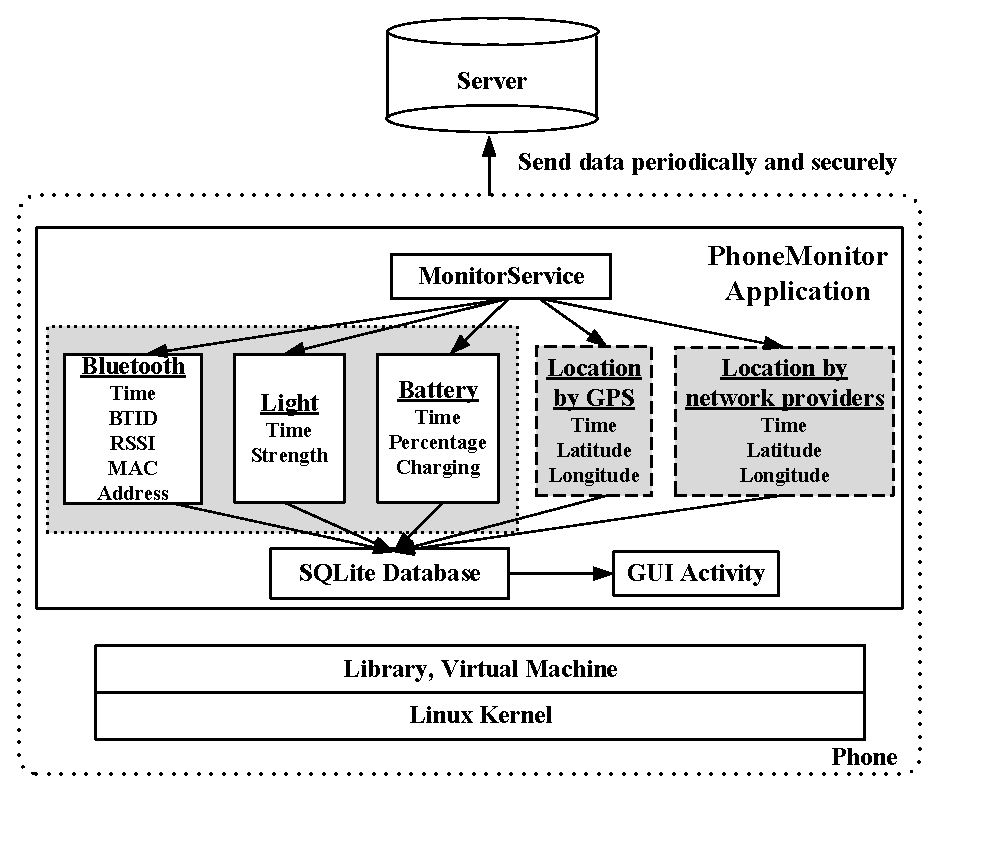
\includegraphics[width=3.5in]{graphs/Figure1.eps}}
\caption{Design of PhoneMonitor} 
\label{fig:agent}
\end{figure} 

\begin{table}[ht] 
\caption{Types of data collected in PhoneMonitor application} 
\centering  
\begin{tabular}{|l|m{10cm}|}
\hline
{\bf Device Information} & Bluetooth, WiFi, Cell, Location, Light Sensor, Screen On/Off, Battery Level, Connection Status, Network Traffic, Application Usage, Port Information, Running/Install Apps, Password, Contacts, Camera Usage\\
\hline
{\bf Digital Communication} & Phone Call, SMS, Mail, Web Browser History, Music\\
\hline
\end{tabular}
\label{table:data} 
\end{table}

Figure~\ref{fig:system} illustrates the framework of smartphone data collection, storage and query process. Data is locally spooled on the phone before being securely transmitted to one of two remote check-in servers.  Data from the check-in server is then spooled locally before being conveyed to a database server not directly connected to the Internet with all accesses strictly logged and validated to protect sensitive user data. From September 2011 to September 2013, we got more than 250G data in the database. 

\begin{figure}[h!tbp]
\centering 
{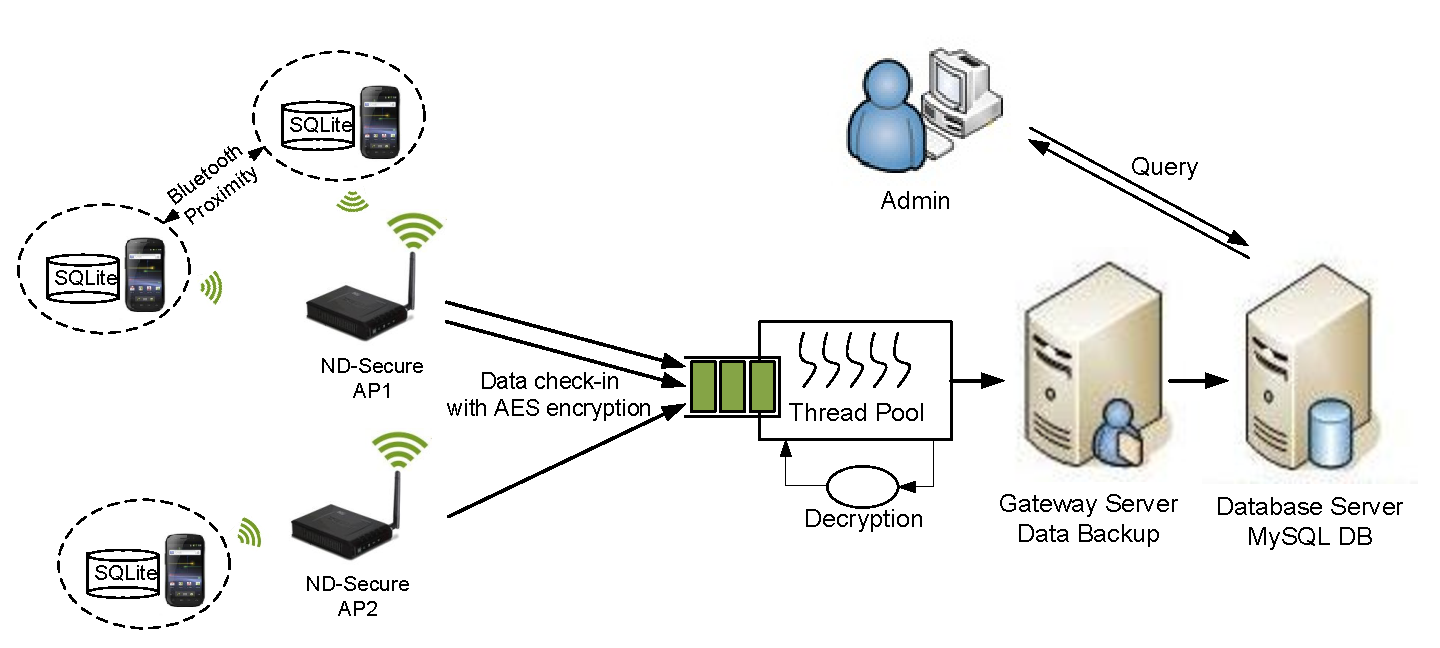
\includegraphics[width=6in]{graphs/system.eps}}
\caption{Smartphone monitoring system} 
\label{fig:system}
\end{figure} 

\section{Dataset Overview}
The dataset used in the dissertation covers 15 months data (Oct 2011 - Dec 2012) and there are around 41 million Bluetooth records, 50 million WiFi scans and 1 million SMS messages. Data from the first two months of the study is excluded to allow for the new freshmen to have settled into a new routine and social arrangements.  A reasonable degree of co-location exists amongst students in the study with students selected clustered amongst six primary dormitories equally divided amongst male and female students.  Once entered into the study, students were free to re-locate at either the beginning of the spring semester (2012) or the start of their sophomore year.  Moreover, the respective distribution levels within individual dormitories made it reasonably close to random chance amongst incoming freshmen for that dormitory if two participants in the study were selected as roommates. At the onset of the monitored period for the paper, approximately 11 students had dropped from the student reducing the data pool to 189 students.  

Table~\ref{table:summary} summarizes the details of the data across different months.  For each of the respective metrics presented in the table, we reduce the sampling rate to five minutes slots scattered throughout the day where each day has the potential for 288 measurement points.  The powered on percentage represents the number of slots when the phone monitor was active with a noticeable drop during later hours (12am - 8 am) but a notable uptick during the evening hours (4pm-12am).  The screen on percentage is the duration when the phone screen is on and implies the average usage of the phone for either consuming data or conducting other communications (SMS, phone call, etc.).  The monthly Bluetooth and WiFi records shows the average number of distinguished Bluetooth devices/WiFi APs detected per device across the month.  University virtual APs are reduced to a single AP as each university router offers between two to four WiFi AP names.  

Figure~\ref{fig:num_cdf} exhibits the empirical distribution functions (ECDF) of different types of data in April 2012 to offer additional context for the data beyond the average values denoted in Table \ref{table:summary}.  Two percentage value ECDFs are plotted (power on, screen on) together with two detected environmental values (unique Bluetooth devices in the month, unique APs in the month).  Scales for each of the two values are the lower axis for percentage and upper axis for raw numeric counts.   Most notably, the average number of unique Bluetooth devices detected in April 2012 was 746 with some devices seeing as high as over 1000 devices and others seeing as low as slightly less than 200 unique devices.  Table~\ref{table:summary} also contains distinctions with respect to intra-study proximity and inter-study breakdowns of the various Bluetooth devices.  As would be expected, intra-study detection dramatically trails off during summer break in tandem with detected university APs as the students leave campus.       

\begin{table}[tb] 
\caption{Monthly Data Summary} 
\centering
\begin{tabular}{p{6cm}|c|c|c|c}
\hline
		  Avg. Monthly Values per Phone							& Nov 2011 & Apr 2012 & Jul 2012 & Nov 2012 \\ [0.5ex] 
\hline\hline Powered On (\%) 										& 73.7 	   & 70.6 	      & 51.3 	& 61.2		\\ 
\hline	  Powered On (\%) (12am-8am) 							&  66.7	    & 60.7 		& 42.3 	& 58.0 \\
\hline 	  Powered On (\%) (8am-4pm) 								& 74.6 	   & 69.3 	      & 51.3 	& 62.7 \\
\hline 	  Powered On (\%) (4pm-12am)   			 				& 79.6	    & 72.7 		& 60.1 	& 62.9 \\
\hline	  Screen On (\%)										&  5.74	    & 5.05 		& 4.99 	& 4.30 \\
\hline	  Total Rx Traffic  (MB)									&  609.2	    & 727.2 	& 864.5 	& 685.8 \\
\hline	  Total Tx Traffic  (MB)									&  133.11	    & 123.8 	& 130.4 	& 200.8 \\
\hline 	  \# of Detected Distinct Bluetooth Devices					&  961 	     & 746 		& 310 	& 681	 \\
\hline 	  \# of Detected Distinct Bluetooth Devices Within Project (RSSI $>=$ -80dBm) 	&  131 	     & 106 		 & 	$<$1 & 75	 \\
\hline	  \# of Detected Distinct WiFi APs 										&  1218 	     & 1004	 	& 1777 	& 1663 \\
\hline	  \# of Detected Distinct WiFi APs in Campus 								&  424 	     & 446	 	& $<$1 	& 433 \\
\hline
\end{tabular}
\label{table:summary} 
\end{table}

\begin{figure}[tbp]
\centering 
{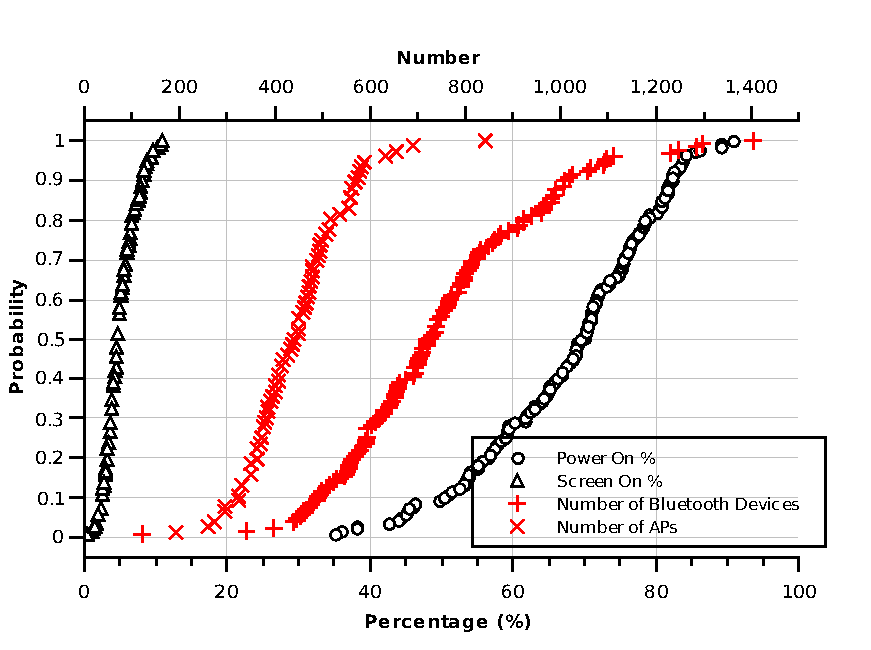
\includegraphics[width=3.5in]{graphs/num_cdf.pdf}}
\caption{ECDF of Data in April 2012} 
\label{fig:num_cdf}
\end{figure} 

\section{Comparison}
The inclusion of a device-side agent on a live user device introduces notable complexity with respect to user privacy and IRB (Institutional Review Board) concerns.  Moreover, such studies tend to be frequently expensive to conduct due to the cost of subsidizing access costs at a sufficient level to yield effective participatory compliance. Although there are several notable wireless datasets including university campuses (MIT Reality~\cite{Nathan3}, UCSD~\cite{mcnett2005access} and Dartmouth~\cite{henderson2004changing}), conference sites (Infocom~\cite{chaintreau2007impact}) and cities (Nokia~\cite{laurila2012mobile}), most datasets are limited in size and scope in terms of capturing dyadic relationships, namely both sides of a potential proximity relationship for the purposes of truly evaluating opportunistic networking.  For instance, both the MIT Reality and Infocom traces record when contact is detected by virtue of Bluetooth discovery, ample for characterizing the inter-contact times but not necessarily capturing energy levels nor traffic needs of the respective nodes.  Alternatively, the UCSD and Dartmouth traces rely on WiFi for localization gathering either data via AP fingerprinting (UCSD) or SNMP logs directly from the AP (Dartmouth).  The richest of the datasets is the data from the Nokia Data Challenge which includes both WiFi and Bluetooth data but the dataset is no longer public after the completion of the analysis.  In contrast to prior works, our dataset includes nominal proximity (Bluetooth) / location data (WiFi, Google Location service) in addition to a complete view of the smartphone environment including WiFi signal strengths, energy levels, traffic demands, and the social context for the participants in the study (Facebook, SMS, etc.).  Table~\ref{table:datasets} summarizes the most relevant studies and compares the works to our own reference study.  

\begin{landscape}
\begin{table*}[t] 
\caption{Dataset Comparison} 
\centering
\scalebox{1}{
\begin{tabular}{c|c|c|c|c|c|c}
\hline
  			Traces 				&  Our Dataset  	&  MIT Reality 	 & 	UCSD 		& Dartmouth 	& Infocom  	& Nokia \\ [0.5ex] 
\hline
\hline		Device  				& Smartphone		&  Cell Phone	 & 	PDA			& Laptop PDA & iMote		&Smartphone \\
\hline		\# of Devices 			& 189			& 97			 & 	275			& 6,648		& 41			& 185\\
\hline		Network Type 			&  Bluetooth/WiFi	& Bluetooth	 &     WiFi			& WiFi 		& Bluetooth	& Bluetooth/WiFi\\
\hline		Contact Type 			& Direct/AP-based	& Direct		 & 	AP-based		& AP-based	& Direct		& Direct/AP-based\\
\hline		Duration (days)			& 458			& 246		 & 	77			& 114		& 4			& 210\\
\hline		Granularity (seconds) 	& 60/300			& 300		 & 	120			& 300		& 120		& N/A\\
\hline		\# of internal contacts 	& 3,616,184 		& 54,667		 &	195,364		& 4,058,284	& 22,459		& N/A\\
\hline		Internal pairwise contact/day	& 0.221		& 0.022		 & 	 0.034		& 0.008		& 3.4		& N/A\\	
\hline		Other proximity related data	& Cell, Traffic, etc.	& Cell	 & 	N/A			& N/A		& N/A		& Cell, etc.\\
\hline
\end{tabular}}
\label{table:datasets} 
\end{table*}
\end{landscape}



%
% Chapter 3
%

\chapter{Bluetooth Proximity}
\label{chap:bt_proximity}

\section{Background}
Interactions are not limited to any particular area and can take place at a wide variety of locations, ranging from sitting and chatting in a Starbucks coffee shop to walking and chatting across a college campus. As will be explored later in the paper, for most face-to-face interactions, the approximate distance between individuals in casual conversation is within 0.5 to 2.5 meters. One of the solutions would seem to be location-based calculation which relies on location technologies such as WiFi triangulation~\cite{wifi}, cell phone triangulation~\cite{cell}, GPS, or a combination of all three. However, none of these solutions are ideal or sufficient. Although WiFi triangulation can present a reasonable degree of accuracy, its accuracy in all but the most dense WiFi deployments is insufficient, ranging on the order of 3 to 30 meters~\cite{wifi}. Similarly, cell phone triangulation suffers from an even worse accuracy~\cite{cell}. Moreover, while WiFi is reasonably pervasive, WiFi tends to generally be sparser in green spaces, i.e. outdoor spaces. Notably, GPS suffers from both an accuracy shortcoming (5-50m) as well as a lack of viability indoors~\cite{survey1}. 

However, it is important to note that face-to-face interaction does not demand an absolute position as offered by the previously mentioned schemes but rather requires a determination of \textit{proximity}. With that important shift of the problem definition, Bluetooth emerges as a straightforward and plausible alternative, offering both accuracy (1-1.2m)~\cite{BTposition} and ubiquity (most modern smartphones come with Bluetooth)~\cite{Nathan2}. Although some prior work has attempted to use the detection of Bluetooth to indicate nearness~\cite{Nathan3}, it is not enough for the face-to-face proximity estimation. The question addressed by this section is to what extent Bluetooth can be an accurate estimator of such proximity.  

\section{Related Work}\label{sec:related work}
Over the years, there has been a number of technologies proposed for proximity detection. Approaches such as those used by Meme Tags~\cite{borovoy1998meme} provide good accuracy but require line of sight. Ultrasound approaches such as Activebadge ~\cite{want1992active} also provide good accuracy but they require infrastructure support. ZigBee technology is widely used in wireless sensor network to provide radio proximity estimation~\cite{baouche2009radio} in the environment where GPS is inoperative. Proximity can also be reported by sounds, and past work has shown audio to be effective for delivering peripheral cues~\cite{mynatt1997audio}. However, it is untenable to expect the use of smartphones to reduce the unobtrusiveness of cues or increase comprehension. For the purposes of this paper, we are interested in techniques that are based on commonly available technologies in smartphones, i.e. GPS, Cell, WiFi and Bluetooth. Particularly, we are interested in techniques that can be applied at the smartphone itself without significant changes to the infrastructure. 

Proximity detection is one of the advanced Location based Service (LBS) functions~\cite{treu2005efficient,kupper2006efficient,vsikvsnys2010private} to automatically detect when a pair of mobile targets approach each other closer than a predefined proximity distance (as in Location Alerts of Google Latitude). For realizing this function the targets are equipped with a cellular mobile device with an integrated GPS receiver, which passes position fixes obtained by GPS to a central location server. Most proposals for such services give low accuracy guarantees and incur high communication costs. Recently, 3-D optical wireless based location approach~\cite{bilgi20103} is proposed which based on both GPS and triangulation technologies. It is another feasible way of utilizing GPS to get relative distance among objects. 

Some proximity estimation methods are based on Cell or WiFi signal. Using Place Lab~\cite{lamarca2005place}, cell phones listen for the MAC address of fixed radio beacons, such as cell tower and wireless access points, and reference the beacons� positions in a cached database. It provides adequate accuracy for detecting something like buddy proximity (e.g., median accuracy of 20-30 meters), but it requires a �wardriving� of the area to obtain pre-mapped cell towers and fixed wireless APs in the area. This can be quite costly, especially keeping the information up to date, as tower positions, etc. are updated on an annual basis. Without calculating absolute location, NearMe~\cite{krumm2004nearme} explores the algorithm for detecting proximity using Wi-Fi signatures (WiFi APs and signal strengths), allowing it to work with no a priori setup. Similarly, ~\cite{li2008peopletones} uses GSM readings to explore the proximity of mobile targets. 

There are some proximity detection works using Bluetooth signal. From a specific work perspective, the works of Nathan et al. ~\cite{Nathan3,Nathan1} are highly relevant to the paper. In those studies, the authors use the ability to detect Bluetooth signals as indicators for people nearby within the Bluetooth range (around 10m). However, such indication does not meet the requirement of face-to-face proximity detection. In class, a student may discuss with others sitting beside him/her, but face-to-face talk is difficult with the students on the other side of the classroom even they are still in the Bluetooth range. Different from the above proximity detection method, our work is a fine grain Bluetooth-based proximity detection method which can provide adequate accuracy for face-to-face proximity estimation without environment limitations. Table~\ref{table:comparison} summarizes the differences of popular techniques, their prominent features and the performance~\cite{survey2,MobileLocation}. 

\begin{table}[ht] 
\caption{Different proximity estimation techniques comparison} 
\centering  
\begin{tabular}{lccc}
\hline
  &Bluetooth & WiFi & GPS \\ [0.5ex] 
\hline\hline HW costs & Medium & High & High\\ 
\hline Coverage & High & High(Indoor) & High (Outdoor)\\
\hline Power Usage & Medium & High & High\\
\hline Accuracy & 1-4m & 2-30m & 5-50m \\
\hline Security & High & High & Not applicable \\	
\hline
\end{tabular}
\label{table:comparison} 
\end{table}

Based on the monitoring system described in Chapter~\ref{chap:dataset}, there are more than one million Bluetooth records collected per week. Figure~\ref{fig:multiphones} shows the distribution of the Bluetooth RSSI values collected from 196 phones in one week (more details will be discussed in Section~\ref{sec:exp} and Section~\ref{sec:case}). The data collected includes both indoor and outdoor environments. As it shows,  the most prevalent value is around -76dBm which indicates much more than 5m indoor and nearly 5m outdoor as will be shown later. Therefore, an unfiltered detection method such as ~\cite{Nathan3,Nathan1} is not enough to estimate the face-to-face proximity and we use a more accurate method in Section~\ref{sec:exp} to solve this problem. Moreover, we introduce various smoothing effects and take advantage of empirical observations to function across a wide variety of typical environments. 

\begin{figure}[h!tbp]
\centering
{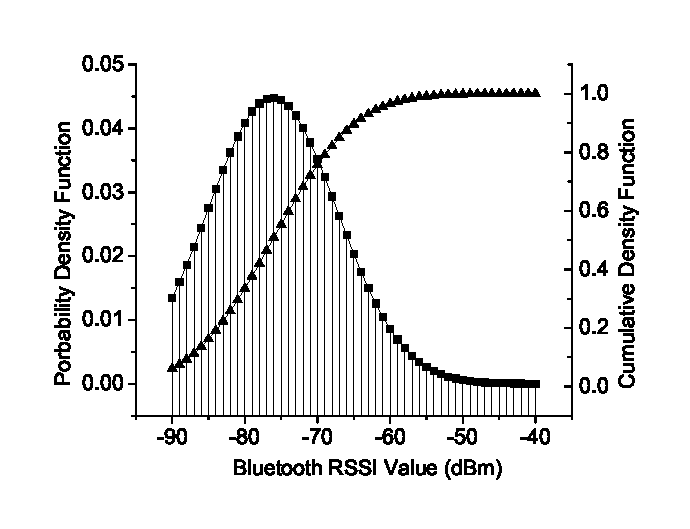
\includegraphics[width=3.4in]{graphs/Figure2.eps}}
\caption{Bluetooth RSSI values distribution in one week} 
\label{fig:multiphones}
\end{figure}

\section{Proximity Estimation Model}\label{sec:exp}
In this section, we explore the relationship between Bluetooth RSSI and distance in real world scenarios. The first method is using RSSI value threshold to determine whether two phones are in proximity or not. The second method introduces the light sensor data to determine whether the phone is indoors or outdoors, inside the backpack or in hand. By differentiating environments and smoothing data, a face-to-face proximity estimation model is outlined to improve the estimation accuracy in general scenarios. At the end of this section the proximity accuracy of Bluetooth, WiFi and GPS are analyzed and compared. 

\subsection{Bluetooth RSSI vs. Distance}
Antti et al. presented the design and implementation of a Bluetooth Local Positioning Application (BLPA)~\cite{BLPA} in which the Bluetooth received signal power level is converted to distance estimate according to a simple propagation model as follows: 
\begin{flalign}
\begin{split}
RSSI  &= P_{TX} + G_{TX} + G_{RX} + 20\log{(\frac{c}{4\pi f})} - 10n\log{(d)}\\
	&= P_{TX} + G -40.2 - 10n\log{(d)}
\end{split}&
\end{flalign}
where \( P_{TX}\) is the transmit power; \(G_{TX}\) and \(G_{RX}\) are the antenna gains; G is the total antenna gain: \(G = G_{TX} + G_{RX}\); \(c\) is the speed of light (\(3.0 * 10^{8}m/s\)); \(f\) is the central frequency (2.44 GHz); \(n\) is the attenuation factor (2 in free space); and \(d\) is the distance between transmitter and receiver (in m). \(d\) is therefore:
\begin{flalign}
\begin{split}
\label{equation: d}
d = 10^{[(P_{TX} - 40.2 - RSSI + G) / 10n]}
\end{split}&
\end{flalign}
However, such a model can only be utilized as a theoretical reference. Due to reflection, obstacles, noise and antenna orientation, the relationship between RSSI and distance becomes more complicated. Our challenge was to assess how much impact these environmental factors have on Bluetooth RSSI values. Therefore, we carried out several experiments to understand how the Bluetooth indicators fade with distance under these environmental influences. 

Indoor experiments were conducted in a noisy hallway (around seven other Bluetooth devices detected) in the campus engineering building. Outdoor experiments were conducted in the open area outside the building. In the measurement there were no obstacles between the two phones and the antennas of the phones were aligned towards each other. In such a way, we tried to build up a relatively simple and ``ideal'' environment where the possible impact factors are reflection and noise only. We repeated the measurements over the period of an hour with the distance being increased by 0.5 meters between each round. Figure~\ref{fig:RSSI} shows the initial fluctuations of indoor RSSI results with different distances. Although the data varies significantly even within the same distance, there is a noticeable gap exists between different distances. Such results further shed light on the viability of using Bluetooth RSSI to indicate the face-to-face proximity.
\begin{figure}[h!tbp]
\centering
{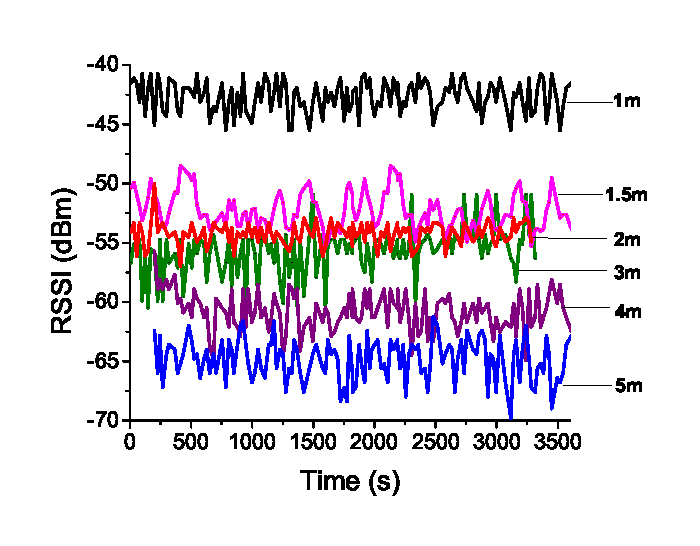
\includegraphics[width=3.5in]{graphs/Figure4.eps}}
\caption{Initial indoor RSSI values with different distances} 
\label{fig:RSSI}
\end{figure}

In Figure~\ref{fig:theory}, we present indoor, outdoor, and theoretical results for Bluetooth across a variety of distances (0-5 meters). The theoretical values were predicted by the propagation model with \(P_{TX}=2.9\ dBm\) and \(G=4.82\ dBi\). These specific values are the average empirical results of our experiment phone. We calculated the average RSSI from nearly 120 raw values for each distance. The indoor results were relatively close to the theoretical values. However, the results outside the building were much farther away from the theoretical reference and imply that these two kinds of environmental settings should be identified in the following measurements.
\begin{figure}[h!tbp]
\centering
{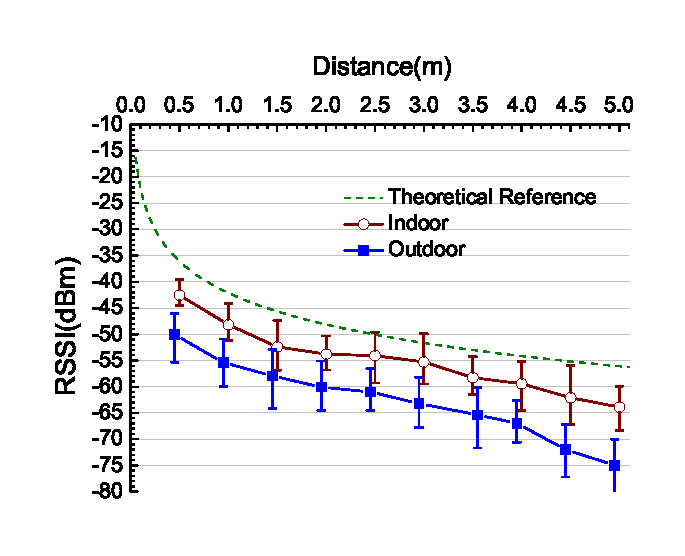
\includegraphics[width=3.5in]{graphs/Figure5.eps}}
\caption{Bluetooth RSSI vs. distance - theoretical, indoor, outdoor} 
\label{fig:theory}
\end{figure}

Furthermore, we performed similar experiments on two phones focusing on the indoor case but with different antenna orientation (e.g. in the same direction) and obstacles (e.g. put in a backpack or partitioned by cubicle) in order to discover the influence of these possible factors. Figure~\ref{fig:inside} illustrates the results with these impacts. The observations include the following: first, the change in orientation turns out to have little impact on the final results. As many smart phones cannot predict phone orientation, antenna design is typically optimized to account for this fact. Second, although we placed two phones on each side of a cubicle board, such an arrangement did not affect RSSI significantly. Third, the most important environmental issue came from the backpack. It may be because the signal of Bluetooth is disturbed or shielded in such a closed environment. As many individuals would be likely to carry their phone in a purse or backpack (particularly on a college campus), the backpack setting bears further investigation. We also recorded the data to check whether the RSSI values on phones are symmetric. Figure~\ref{fig:inside_reverse} shows the RSSI values on one phone are almost the same as the results on the other phone. 
\begin{figure}[h!tbp]
\centering
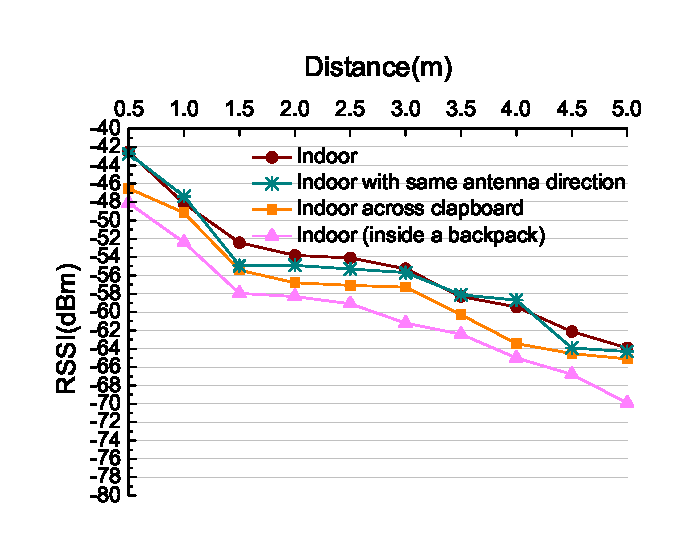
\includegraphics[width=3.5in]{graphs/Figure6.eps}
\caption{Bluetooth RSSI vs. Distance indoor case} 
\label{fig:inside}
\end{figure}

\begin{figure}[h!tbp]
\centering
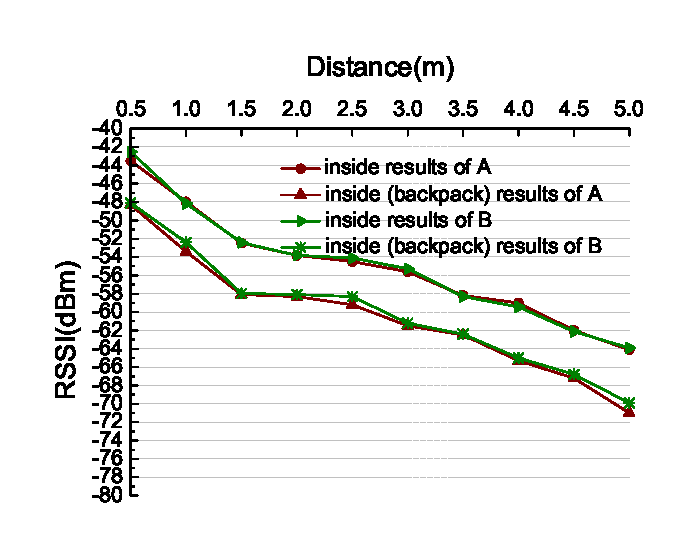
\includegraphics[width=3.5in]{graphs/Figure7.eps}
\caption{Symmetric RSSI values} 
\label{fig:inside_reverse}
\end{figure}

Using the same method, we measured the RSSI values outdoors with the consideration of the influence of a backpack. Figure~\ref{fig:outside} shows the results from those experiments. Similarly, the RSSI values become lower when the phones are in the backpack so it is a non-ignorable element in the following estimations, further reinforcing that detection of such an arrangement may be critical for proper distance estimation resolution.

\begin{figure}[h!tbp]
\centering
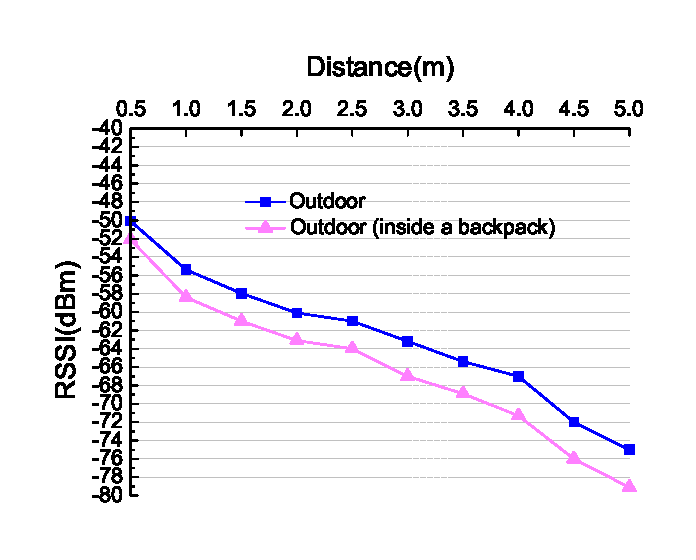
\includegraphics[width=3.5in]{graphs/Figure8.eps}
\caption{Bluetooth RSSI vs. Distance outdoor case} 
\label{fig:outside}
\end{figure}

Based on these indoor and outdoor results, there are two main environmental factors that may effect the RSSI values: inside/outside building and inside/outside a backpack. Besides those factors, it is also necessary to take multiple-phones scenario into consideration since phones with Bluetooth around may have interference on Bluetooth RSSI values. 

\subsection{Proximity Estimation Model}
As mentioned in the beginning, we aim to provide an accurate proximity estimation for face-to-face communication. This raises a question: what is the face-to-face communication distance? In this subsection, we first define the face-to-face distance and then use the indoor results as a threshold to do the estimation in real world scenarios. Since the error rate of using a simple threshold is relatively high, we explore the possible reasons and propose a proximity estimation model with the introduction of light sensor values. 

\emph{Distance of face-to-face communication:}
When we have dinner with our friends sitting at the same table, the conversation among us is called face-to-face communication; or when we talk with someone side by side, the distance between us is also called face-to-face communication. In other words, face-to-face communication happens when people are close enough to have conversations in a convenient manner. People typically have such communication when they are sitting or walking together. Thus, we calculate the distance for this kind of communication by measuring distances across the campus (such as diagonal of desk in dinning hall, distance between desks in classrooms and etc.) and the average value is equal to 1.52m. The detailed samples are listed in Table~\ref{table:distance}. 

\begin{table}[ht] 
\caption{Distance of face-to-face communication around campus} 
\centering  
\begin{tabular}{lccc}
\hline
\multicolumn{1}{c}{Place} & Distance(cm) \\ [0.6ex] 
\hline\hline Diagonal of small square desk in La Fortune & 116\\ 
\hline Diagonal of large square desk in La Fortune & 160\\
\hline Diameter of round desk in La Fortune & 120\\
\hline Diagonal of desk in dinning hall & 250\\
\hline Distance between desks in Cushing office & 125\\
\hline Distance between desks in classroom & 155\\
\hline Diagonal of desk in discussion cubic & 220\\
\hline Distance between people walking side by side & 70\\	
\hline
\end{tabular}
\label{table:distance} 
\end{table}

To conduct an evaluation of the accuracy of our Bluetooth method, we constructed a scenario that draws upon several likely occurrences in normal campus interactions. The scenario blends each of the earlier test cases and provides data to assess the accuracy in a real-world setting. 
The measurement was conducted as follows: two people with two phones walked side by side from Cushing Hall to Grace Hall and then returned back (Figure~\ref{fig:map}).

\begin{figure}[h!tbp]
\centering
{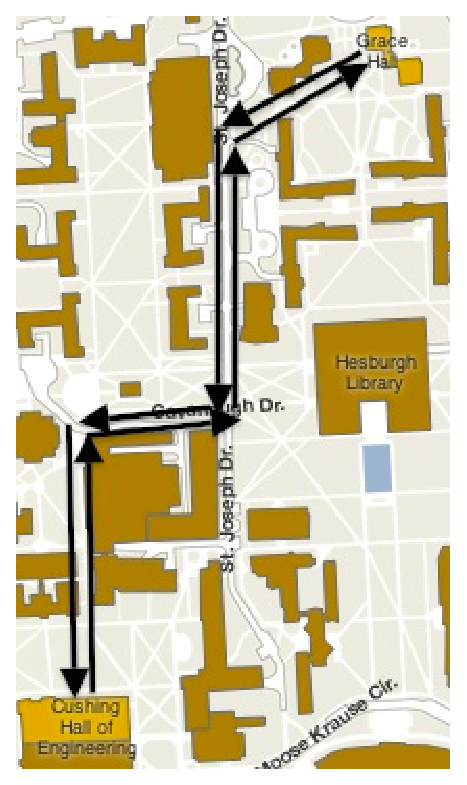
\includegraphics[width = 2.2in]{graphs/Figure9.eps}}
\caption{Walk path for real-world scenario} 
\label{fig:map}
\end{figure} 

The whole process took 40 minutes and individuals were always within the distance for face-to-face communication. The Bluetooth update time interval was changed to 10 seconds temporarily in order to provide enough samples. During the first ten minutes (phone in hand) and last ten minutes (phone inside a backpack) individuals were inside Cushing Hall. When individuals were outside (the duration was 20 minutes), in the first ten minutes individuals held the phones in their hands and then put the phones in their backpack for the later ten minutes. 

\emph{Single Threshold:} 
After data collection, the corresponding RSSI value (-52dBm) of direct communication distance (152cm) based on the indoor measurements (Figure~\ref{fig:inside}) was used as a threshold to estimate whether the individuals were in proximity. Accordingly, values less then \mbox{-52dBm} were considered as not in face-to-face proximity and labeled as a wrong estimation.

\begin{table}[ht] 
\caption{Error rate against real-world data} 
\centering  
\begin{tabular}{lccc}
\hline\hline 
Total samples & 246 \\ [0.6ex] 
\hline Total error rate & 72.8\%\\ 
\hline Indoor error rate (0 - 10 mins) & 14.3\%\\
\hline Outdoor error rate (10 - 20 mins) & 91.3\%\\
\hline Outdoor (inside a backpack) error rate (20 - 30 mins) & 100.0\%\\
\hline Indoor (inside a backpack) error rate (30 - 40 mins)  & 85.0\%\\	
\hline
\end{tabular}
\label{table:naive} 

\end{table}
\begin{table}[ht] 
\caption{Improved error rate with modified threshold} 
\centering  
\begin{tabular}{lccc}
\hline\hline 
Total samples & 246 \\ [0.6ex] 
\hline Total error rate & 48.4\%\\ 
\hline Indoor error rate (0 - 10 mins) & 4.9\%\\
\hline Outdoor error rate (10 - 20 mins) & 53.2\%\\
\hline Outdoor (inside a backpack) error rate (20 - 30 mins) & 85.5\%\\
\hline Indoor (inside a backpack) error rate (30 - 40 mins)  & 49.2\%\\	
\hline
\end{tabular}
\label{table:naive2} 
\end{table}

Table~\ref{table:naive} shows the results and error rate of this na\"{\i}ve method. It was found that both of the outdoor and backpack parts have extremely high error rates. After switching the threshold value to -58dBm which is the outdoor RSSI values with 152cm distance,  the error rate was improved but still high as shown in Table~\ref{table:naive2}.

In our opinion, the reasons for high error rates include: 
\newline i) One fixed threshold is not enough as the indicator of correct or wrong estimation; 
\newline ii) Only indoor or outdoor relationship was used to analyze the data without differentiation; 
\newline iii) The influence of backpack and other possible environmental interference were not taken into consideration; 
\newline iv) Each RSSI value was not smoothed to allow for environmental fluctuations.

\emph{Multiple Thresholds:} 
According to the reasons for high error rate analyzed above, we introduce the proximity estimation model which is a multiple threshold-based method with the consideration of data smoothing and different environmental effects.
\vspace{2mm}

i) Data Smoothing

Since there is time delay during the data collection, we do smoothing on the data collection to avoid environmental fluctuation effects and there are several ways to achieve it. One way is using simple window function and each value \(RSSI_{i}\) at time \(i\) is modified using the following function:
\begin{flalign}
\begin{split}
RSSI_{i}=a* RSSI_{i-1} + b* RSSI_{i} + c* RSSI_{i+1}
\end{split}&
\end{flalign}
For the values of the parameters (a, b and c), several combinations such as (0.4, 0.6, 0), (0.3, 0.4, 0.3) and (0.2, 0.6, 0.2) are used in the following comparisons. 
Another smoothing method is to utilize EWMA (exponentially weighted moving average) to analyze the dataset. Let \(E_{i}\) be the EWMA value at time \(i\) and \(s\) be the smoothing factor. The EWMA calculation is as follows:
\begin{flalign}
\begin{split}
E_{i}=s* RSSI_{i} + (1-s)E_{i-1}
\end{split}&
\end{flalign}
Based on real-world data as shown in Table~\ref{table:naive2}, we combine the data smoothing method with signal threshold filter to analyze the effects of data smoothing and select the best smoothing function. In Table~\ref{table:smoothing}, we compare three different combinations for window function and two types of smoothing factors. While the combination (0.3, 0.4, 0.3) exhibits good improvement of error rate in different scenarios compared with results in Table~\ref{table:naive2}, the EWMA methods with smoothing factor 0.5 is the best among the five options and we use it in the proximity estimation model.

\begin{table}[ht] 
\caption{Improved error rate with data smoothing} 
\centering
\begin{tabular}{|c|c|c|c|c|c|}
\hline 
& \multicolumn{3}{c|}{Simple Window Function} & \multicolumn{2}{c|}{EWMA}\\
\hline
& (0.4, 0.6, 0) & (0.3, 0.4, 0.3) & (0.2, 0.6, 0.2) & s = 0.5 & s = 0.8\\
\hline Total& 49.6\% & 28.3\% & 37.1\% & 26.8\% & 38.2\%\\ 
\hline Indoor & 5.4\% & 3.4\% & 5.7\% & 2.1\% & 4.9\%\\
\hline Outdoor & 50.8\% & 39.4\% & 42.3\% & 23.8\% & 34.7\%\\
\hline Outdoor backpack & 82.9\% & 59.3\% & 76.8\% & 61.2\% & 79.1\%\\
\hline Indoor backpack & 50.7\% & 30.2\% & 45.7\% & 27.5\% & 48.3\%\\	
\hline
\end{tabular}
\label{table:smoothing} 
\end{table}

ii) Light Sensor Data

As shown in Figure~\ref{fig:inside} and Figure~\ref{fig:outside}, the Bluetooth RSSI values are much smaller than the indoor ones when the phone is in the backpack or outdoors. One of our observations is that it is possible to treat the light sensor data as an indicator of the environment. Figure~\ref{fig:light} reveals the light sensor data distribution in different settings: during the daytime when the phone is inside the building the light sensor returns values between 225 to 1280; while this value comes up to larger than 1280 when phone is under daylight. When the phone is in the backpack, the light values are typically around 10.  Therefore, when the light sensor value is in a range that indicates the phone is in a specific corresponding environment. 

In Figure~\ref{fig:walkdata}, we reviewed the distribution of the Bluetooth RSSI values collected in the walk experiment and the corresponding light sensor data got at the same time. As shown, there is RSSI data fluctuation even in the same setting due to the interference and noise. However, most Bluetooth RSSI values are larger than -55dBm when light sensor data is from 225 to 1280 (indicates indoor setting) while the RSSI values are smaller than -55dBm when light sensor data is in other zones (either in the backpack or outdoors). 

\begin{figure}[h!tbp]
\centering
{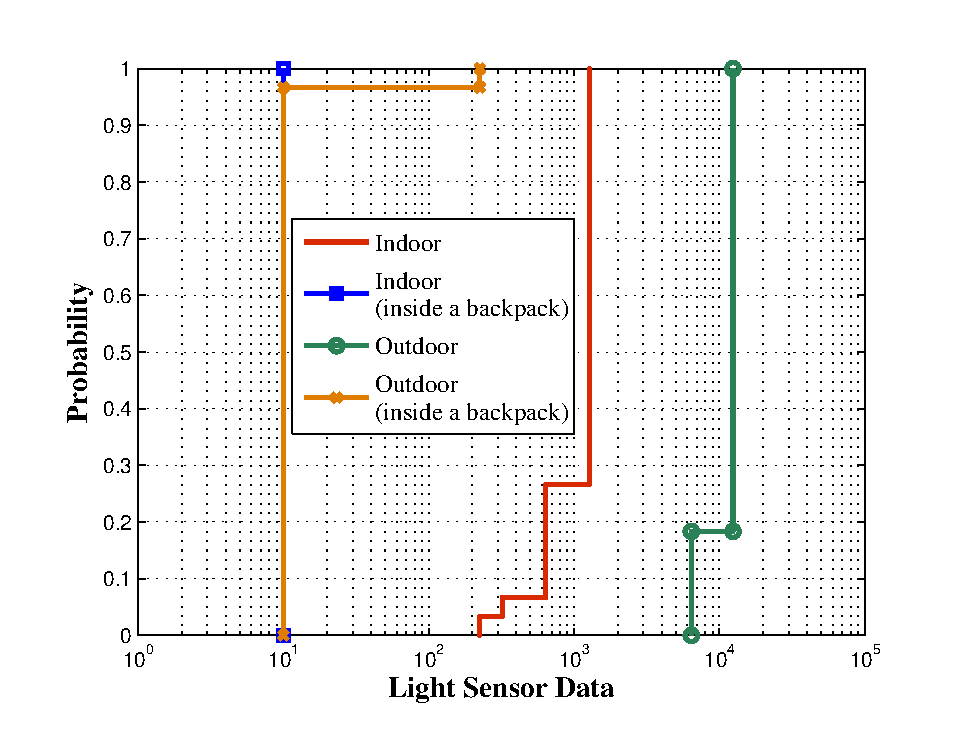
\includegraphics[width=3.5in]{graphs/Figure10.eps}}
\caption{Cdf of light sensor data in different environments} 
\label{fig:light}
\end{figure} 

\begin{figure}[h!tbp]
\centering
{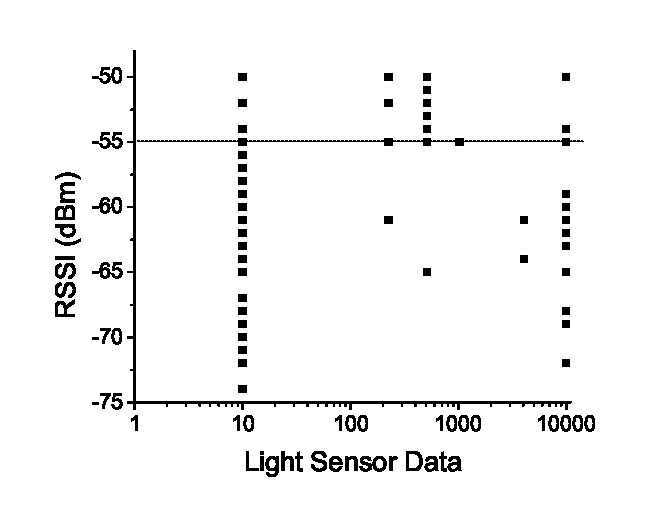
\includegraphics[width=3.5in]{graphs/Figure11.eps}}
\caption{Data in Real-world Scenario} 
\label{fig:walkdata}
\end{figure} 

Thus, light sensor data is introduced to differentiate the circumstances to improve the accuracy of distance estimation based on the rules in Table~\ref{table:light}. Variations due to time of day (day vs. evening) may be accounted for using the smartphone time. Inevitably, accuracy will decrease during evening hours but we felt this is an adequate tradeoff for improved environmental detection. Unfortunately, the Nexus S 4G phone does not contain a pressure sensor which could be used to further improve results.  

\begin{table}[ht] 
\centering
\caption{Environment Estimation with Light Sensor Data}
\begin{tabular}{cc}
\hline\hline 
Light Sensor Data & Environment Estimation\\ [0.3ex] 
\hline (0, 100] & Inside backpack\\
\hline (100, 1280] & Indoor and out of backpack\\
\hline $>$1280 & Outdoor and out of backpack\\
\hline
\end{tabular}
\label{table:light} 
\end{table}

iii) Proximity Estimation Model

Based on the analysis of noise and interference, we use a multiple threshold model instead of a single threshold to do the proximity estimation. In Figure~\ref{fig:theory}, the corresponding indoor RSSI values of 2.5m (the maximum distance for face-to-face communication) is around -55dBm. It is obvious that when the received RSSI value is larger than -55dBm the two phones are in face-to-face proximity. Similarly, when the outdoor RSSI values is larger than -60dBm the two phones holder are close enough to have direct interaction. We call such data zone the \textit{``Positive Zone"} denoting where two individuals are certainly within face-to-face interaction distance.

For the indoor data smaller than -55dBm, the model is constructed based on the following observation: in Figure~\ref{fig:inside} the smallest value for 5m distance in the test was -65dBm and it had a relatively low probability of occurence (values larger than -65dBm is less than 20\%) in Figure~\ref{fig:multiphones}. Taking noise and interference into consideration, the value between -65dBm and -55dBm may also indicate a face-to-face proximity with high probability. Figure~\ref{fig:multiphones} includes both indoor and outdoor data and the most frequent data is -76dBm and the lowest values detected is -90dBm. When the indoor data is in (-76dBm, -65dBm), it is still possible to make a face-to-face communication but the probability is relatively low. The indoor data smaller than -76dBm implies that it is too far to have a direct communication and it is called the \textit{``Negative Zone"}. Similarly, we set up several bounds for outdoor data: the smallest value for 5m is -75dBm. Therefore the zone(-75dBm, -60dBm) has a relatively high probability while the zone(-90dBm, -75dBm) is the low probability zone. When the outdoor data is smaller than -90dbm, we strongly believe it is impossible to indicate a face-to-face proximity or even be detected. 

Furthermore, we revisit the data regarding the inside backpack environment. Based on light sensor data, it is difficult to distinguish indoor or outdoor when the phone is inside the backpack. We noticed that when distance are 2.5m and 5m, the corresponding indoor Bluetooth RSSI values inside a backpack are -59dBm and -70dBm and the corresponding outdoor values are -64dBm and -79dBm. We defined the zone which is larger than -59dBm as \textit{``Positive Zone"} for backpack data. Similarly, the zone which is smaller than -79dBm as \textit{``Negative Zone"}. For the data between the two above bounds, we also define \textit{``High Probability (HP) Zone"} (-70dBm, -59dBm) and \textit{``Low Probability (LP) Zone"} (-79dBm, -70dBm). Therefore, for each type of environment, we have four zones as summarized in Table~\ref{table:distribution}. Table~\ref{table:multithresholds} lists the corresponding multiple thresholds. Figure~\ref{fig:distribution} illustrates the multiple thresholds of different zones in a more direct way. 

For high and low probability zones, we name the minimum values in low probability zone as \textit{B$_{min}$}, the maximum value in high probability zone as \textit{B$_{max}$} and the range as \textit{B$_{range}$}. Therefore B$_{range}$ = B$_{max}$ - B$_{min}$. To sum up, a proximity estimation model with multiple thresholds is proposed to improve the accuracy. For Bluetooth RSSI value \textit{x$_i$} and the corresponding light sensor value \textit{y$_i$} at time \textit{i}, we calculate the probability of face-to-face proximity \textit{p$_i$} as described in algorithm~\ref{algo:procedure}.

\begin{table}[ht] 
\centering
\caption{ Definition of Zones in Different Environments} 
\begin{tabular}{lccc}
\hline\hline 
Zones &  Indoor & Outdoor & Inside Backpack \\ [0.3ex] 
\hline Positive & $>$=B$_{I\_FTF}$ & $>$=B$_{O\_FTF}$ & $>$=B$_{I\_P\_FTF}$\\
\hline HP & [B$_{I\_5m}$, B$_{I\_FTF}$) & [B$_{O\_5m}$, B$_{O\_FTF}$) & [B$_{I\_P\_5m}$, B$_{I\_P\_FTF}$)\\
\hline LP & [B$_{frequent}$, B$_{I\_5m}$) & [B$_{min}$, B$_{O\_5m}$) & [B$_{O\_P\_5m}$,B$_{I\_P\_5m}$)\\
\hline Negative & $<$B$_{frequent}$ & $<$B$_{min}$ & $<$B$_{O\_P\_5m}$\\
\hline
\end{tabular}
\label{table:distribution} 
\end{table}

\begin{table}[ht] 
\centering
\caption{Boundary Summary}
\begin{tabular}{llc}
\hline\hline 
Boundary &  \multicolumn{1}{c}{Detail} & Values(dBm) \\ [0.3ex] 
\hline B$_{I\_FTF}$& Indoor fact-to-face (2.5m) & -55\\
\hline B$_{O\_FTF}$& Outdoor fact-to-face (2.5m) & -60\\
\hline B$_{I\_P\_FTF}$& \parbox[t]{3cm}{Indoor inside backpack fact-to-face (2.5m)} & -59\\
\hline B$_{O\_P\_FTF}$& \parbox[t]{3cm}{Outdoor inside backpack fact-to-face (2.5m)}& -64\\
\hline B$_{I\_5m}$& Indoor 5m & -65\\
\hline B$_{O\_5m}$& Outdoor 5m & -75\\
\hline B$_{I\_P\_5m}$& Indoor inside backpack 5m & -70\\
\hline B$_{O\_P\_5m}$& Outdoor inside backpack 5m & -79\\
\hline B$_{frequent}$& Most frequent value in the results& -76\\
\hline B$_{min}$& Minimum in the results & -90\\
\hline
\end{tabular}
\label{table:multithresholds} 
\end{table}

\begin{figure}[h!tbp]
\centering
{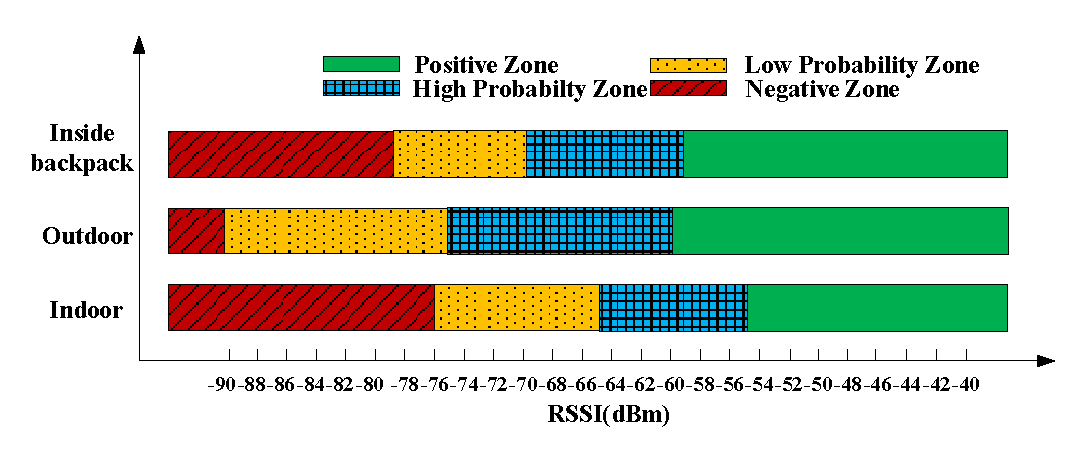
\includegraphics[width=6in]{graphs/Figure12.eps}}
\caption{Multiple Thresholds in Different Zones} 
\label{fig:distribution}
\end{figure} 

\begin{algorithm}
\caption{Estimate probability $p_i$ of face-to-face proximity with Bluetooth RSSI value $x_i$ and light sensor value $y_i$}
\begin{algorithmic} 
\STATE $x_i \leftarrow a*x_{i-1} + b*x_i + c*x_{i+1}$
\STATE determine the scenario depending on $y_i$
\IF{$x_i\ is\ in\ positive\ zone$}
\STATE $p_i \leftarrow 1$
\ELSIF{$x_i\ is\ in\ probability\ zone\ [B_{min}, B_{max})$}
\STATE $p_i \leftarrow (x_i-B_{min})/B_{range}$
\ELSE
\STATE $p_i \leftarrow 0$
\ENDIF
\end{algorithmic} 
\label{algo:procedure} 
\end{algorithm}

We define \textit{Required Accuracy} (RA) as the lowest requirement for the probability to indicate two phones are in face-to-face proximity. With the improved estimation model, we analyze the data in the real-world scenario again and the error rate is improved greatly as shown in Table~\ref{table:improved}. Once \textit{p$_i$} is higher than 45\% ( RA = 45\%), the two phones are considered to be in the face-to-face proximity. The bigger the RA value is, the more accurate face-to-face proximity we can obtain. We choose 45\% as RA based on the following calculation: in each type of environment, the probability of the lowest possible value \textit{l} in high probability zone equals to (l-\textit{B$_{min}$}) divided by \textit{B$_{range}$}. The smallest one in three types of environments equals to 45\%.

\begin{table}[ht] 
\caption{Error rate against real-world data with proximity estimation model} 
\centering  
\begin{tabular}{lccc}
\hline\hline 
Total samples & 246 \\ [0.5ex] 
\hline Total error rate & 4.3\%\\ 
\hline Inside error rate (0 - 10 mins) & 0.0\%\\
\hline Outside error rate (10 - 20 mins) & 4.5\%\\
\hline Outside (inside a backpack) error rate (20 - 30 mins) & 8.3\%\\
\hline Inside (inside a backpack) error rate (30 - 40 mins)  & 6.2\%\\
\hline
\end{tabular}
\label{table:improved} 
\end{table}

\subsection{Comparisons}

WiFi triangulation/trilateration is a widely used method to do location indoors while GPS is perhaps the most popular way to do location outdoors. As summarized in Section~\ref{sec:related work}, both of them have their own advantages and disadvantages. Here we use WiFi and GPS to do the face-to-face proximity estimation in order to compare the accuracy of them with the Bluetooth method we proposed. Together with the power consumption comparison in Section~\ref{sec:system}, the method of Bluetooth is proved to be an effective and efficient way in both aspects of accuracy and power usage. 

We collected both network-provider location and GPS location data on the phone for the comparison. With the API provided by class \textit{LocationManager} in Android SDK, we can get both kinds of location data by choosing different location providers with the frequency of three minutes. The GPS provider determines location using satellites while the network provider determines location based on availability of cell tower and WiFi access points(APs). In the network provider method, the triangulation is used to get the location of the phone with the knowledge of cell towers' or APs' locations. When each phone's location is known, the relative distance as well as the accuracy is easy to calculate. 
\newline\indent We conducted the experiment on a game day in the campus. Two students (A and B) went to Notre Dame Stadium to watch the game together. In Figure~\ref{fig:wifi_gps} the reported location data are marked. From 3pm to 7pm, the location data recorded by network provider are (41.699517, -86.232877) and (41.699203, -86.235269). During the same time period, the GPS provider collected the location as (41.699504, -86.234624) and (41.699004, -86.235723). The corresponding distance between the reported data were 11.25 meters (443 inches) and 7.92 meters (312 inches) respectively. Based on the results reported by the phones, the accuracy of WiFi-based localization turns out to be around 10-15 meters and the one using GPS is around 10 meters. 

\begin{figure}[h!tbp]
\centering
{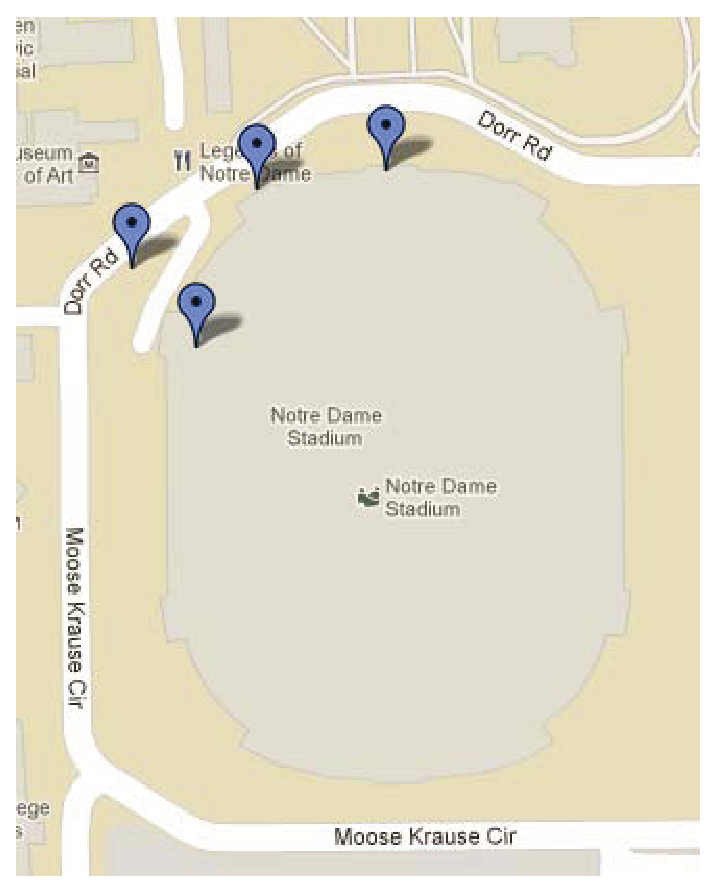
\includegraphics[width=2.5in]{graphs/Figure13.eps}}
\caption{Location data provided by WiFi and GPS} 
\label{fig:wifi_gps}
\end{figure} 

Compared to the above WiFi triangulation and GPS methods, the Bluetooth-based method was more suitable for the face-to-face proximity estimation. As we mentioned before, there is no need to get the absolute location data to calculate the distance. Instead, we only need relative distance to do the estimation. From 3pm to 7pm on that day, we collected the Bluetooth RSSI on both phones and used the estimation model to do the analysis. When RA is 45\%, we got the error rate around 6\% with 554 sample data. Table~\ref{table: comparison2} summarizes the comparison results of accuracy and power consumption percentage by invoking each method with similar frequency. Compared with WiFi and GPS, out method is accurate enough to indicate the face-to-face proximity. At the same time, the power consumption is at least 40\% less than the other two technologies.  These results are consistent with the data in Table~\ref{table:comparison} and Bluetooth can definitely fulfill the requirements of proximity estimation in our system. 

\begin{table}[ht] 
\caption{Accuracy and power consumption comparisons} 
\centering  
\begin{tabular}{llcc}
\hline
  &\multicolumn{1}{c}{Accuracy} & Power consumption & Samples\\[0.5ex] 
\hline\hline Our method & 1.5 - 2.5 meters & 15.7\% & 554\\
\hline WiFi & 10-15 meters & 25.7\% & 251\\
\hline GPS & 10 meters & 58.6\% & 98\\	
\hline
\end{tabular}
\label{table: comparison2} 
\end{table}

\section{Case Study}\label{sec:case}

While our experimental data shows the viability of Bluetooth as a proximity estimation tool, we examine the larger corpus of data from our smartphone study. We gathered high-fidelity data set by deploying the ``PhoneMonitor" app on the Nexus S 4G android phones of 196 users. The participants were randomly chosen from the 2011 freshmen in the University of Notre Dame and were given the phones with unlimited voice, text and data plans. We encouraged the users to take advantage of all the features and services of the phone. The data set, including Bluetooth RSSI, WiFi RSSI, light sensor values as well as locations, was gathered between Sep and Oct 2011. With the data collected on these phones, we used the face-to-face proximity estimation model to get people who are in the direct communication distance with other participants. In the previous section, we showed that the proximity estimation model with multiple thresholds can increase the accuracy of proximity estimation effectively. In the following subsections, more cases and samples will be introduced to explore the Bluetooth-based method for proximity estimation in daily life. 

\subsection{Proximity in large group}
With the data reported by 196 phones over two months, we analyzed the proximity among a large group. We first used Table~\ref{table:week} to show the proximity variation in one week (Oct 3rd - Oct 9th). There are three columns in the table: \textit{Proximity Detected} column is the total number of devices which at least detected one of the other devices with face-to-face proximity probability larger than 45\% (RA = 45\%); \textit{Maybe Detected} column stands for the number of devices which detected other devices but most of them were in the low probability zone as shown in Table~\ref{table:distribution}; \textit{None} column is number of devices which do not report any data or the detected Bluetooth RSSI values were always in the negative zone. The number of samples may be varied from day to day. 

Notably, the weekend included a home football game. Compared to the weekdays, more ``Proximity Detected" cases are reported on Saturday since many students watched the game together and sit in the same student zone. On Sunday, we observed significant  "None" cases which may indicate students stayed in their room or went home instead of interacting.

\begin{table}[ht] 
\caption{Proximity variation in a week} 
\centering  
\begin{tabular}{ccccc}
\hline
  & Num of Devices & Proximity Detected & Maybe Detected & None\\[0.5ex] 
\hline\hline Mon & 190 & 93 & 94 & 3\\
\hline Tue & 193 & 108 & 84 & 1\\
\hline Wed & 192 & 107 & 84& 1\\
\hline Thu & 192 & 106 & 86 & 0\\
\hline Fri & 191 & 112 & 76 & 3\\
\hline Sat & 194 & 129 & 61 & 4\\
\hline Sun & 190 & 71 & 68 & 51\\
\hline
\end{tabular}
\label{table:week} 
\end{table}

We look into the data on Tuesday in a more detailed way. Before we reveal the proximity variation on that day, we first plot the distribution of reported light sensor data and Bluetooth RSSI values in order to compare them with the former results we received in two-phones scenario. Figure~\ref{fig:light_tuesday} shows the trend of light sensor values in 24 hours. During the early morning and late night, most values were smaller than 1000 which means the participants are inside the buildings.  From 8am to 8pm we noticed many values larger than 10000. At the same time, several values at the bottom (values vary from 10 to 100) indicate the phone is in the backpack. Since the light sensor values are not reliable to indicate indoor or outdoor during nighttime, we focus on the proximity variation during the daytime. Using the same method as above, we summarize the proximity variation on that day in Table~\ref{table:tuesday}. The number of "Proximity Detected" cases during the class time (8am-5pm) is more than the one of after class time. Specially, the devices met much more other devices during the lunch time than the other time durations. 

\begin{figure}[h!tbp]
\centering
{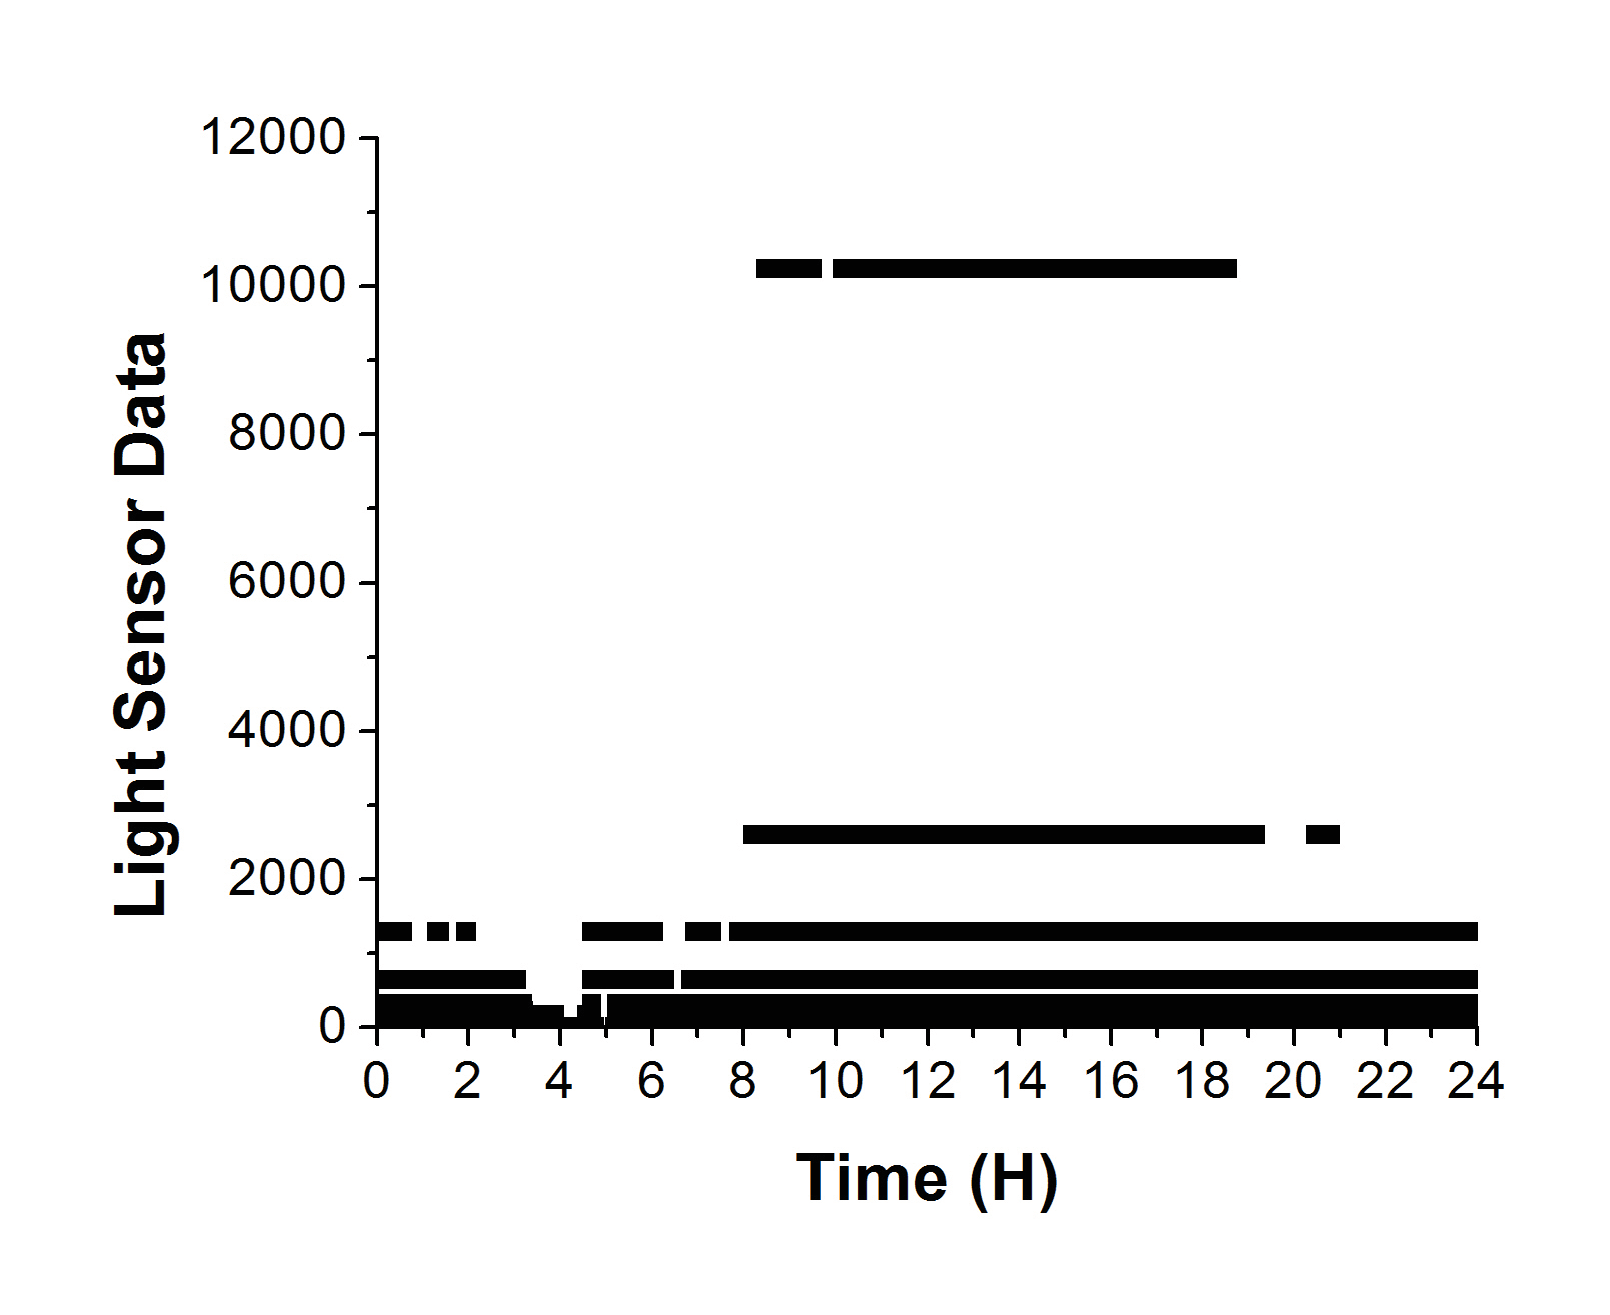
\includegraphics[width=3.5in]{graphs/Figure14.eps}}
\caption{Light sensor data distribution on Tuesday} 
\label{fig:light_tuesday}
\end{figure}

\begin{table}[ht] 
\caption{Proximity variation on Tuesday Daytime} 
\centering  
\begin{tabular}{cccc}
\hline
 & Proximity Detected & Maybe Detected & None\\[0.5ex] 
\hline\hline 8am-11am & 90 & 89 & 14\\
\hline 11am-2pm & 101 & 82 & 10\\
\hline 2pm-5pm & 89 & 97 & 7\\
\hline 5pm-8pm & 84 & 98 & 11\\
\hline
\end{tabular}
\label{table:tuesday} 
\end{table}


Figure~\ref{fig:bt_tuesday} reflects the distribution of Bluetooth RSSI values on that day. The most frequently value is around -75dBm which is similar as concluded in Figure~\ref{fig:multiphones}. As revealed in Section~\ref{sec:exp}, when RSSI value is smaller than -75dBm, it has a relatively low probability that the two phones are in face-to-face proximity. 
Critically, a method such as the one in ~\cite{Nathan3,Nathan1} would misdetect such interactions. Based on both Bluetooth RSSI values and light sensor values, our model can improve the accuracy of face-to-face proximity indication. 

\begin{figure}[h!tbp]
\centering
{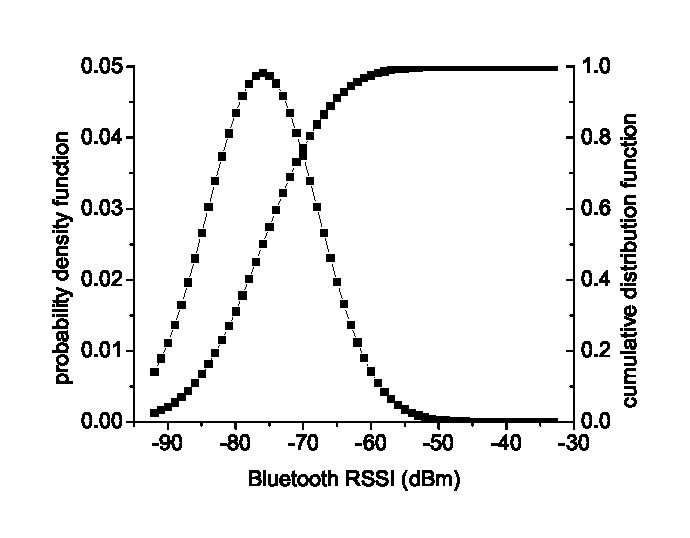
\includegraphics[width=3.5in]{graphs/Figure15.eps}}
\caption{Bluetooth RSSI values distribution on Tuesday} 
\label{fig:bt_tuesday}
\end{figure}

\subsection{Proximity in small group}

\subsubsection{Football Game Day}
In 2011, the university had a football game with Air Force which lasted for four hours. There were 126 students among the 196 that watched the game in the stadium and we gathered 56710 Bluetooth records in the database. In Figure~\ref{fig:018},  we select one participant \textit{S018} and show the detected phones around that student through Bluetooth during the 4 hour period. For every five minutes, if any other phone is detected we add its corresponding ID in that time slot. There are total 48 time slots and with several students always together with the student in the game. Similarly, we explore one of those nearby students \textit{S077} to validate symmetric detection in Figure~\ref{fig:077}. These two figures further show that it is practical to use Bluetooth to detect people around. 
\begin{figure}[h!tbp]
\centering
{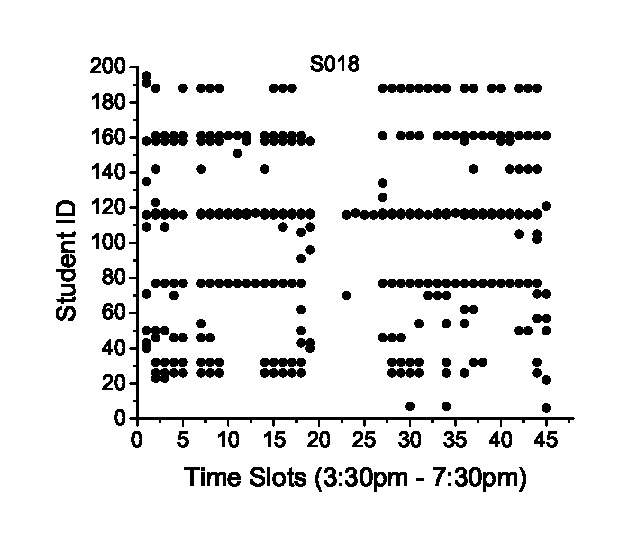
\includegraphics[width=3.5in]{graphs/Figure16.eps}}
\caption{\textit{S018} data on game day} 
\label{fig:018}
\end{figure} 

\begin{figure}[h!tbp]
\centering
{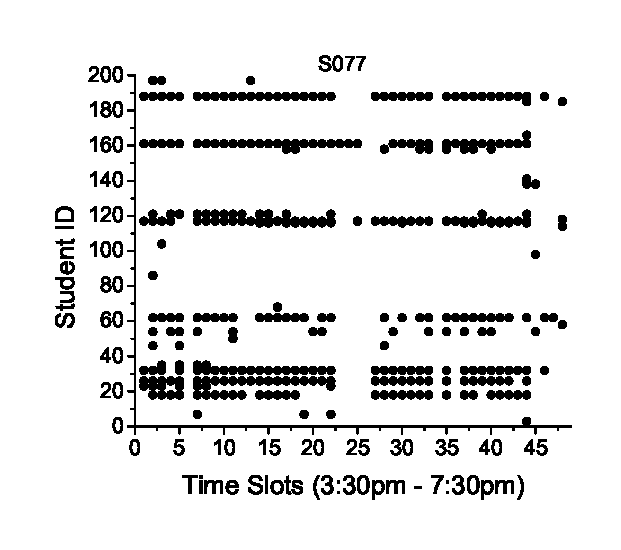
\includegraphics[width=3.5in]{graphs/Figure17.eps}}
\caption{\textit{S077} data on game day} 
\label{fig:077}
\end{figure} 

Figure~\ref{fig:018} shows the detected students around without any restriction of Bluetooth RSSI values. In order to get list of the students in face-to-face proximity, we need to utilize the proximity estimation model to refine the results. Combined with light sensor data and method of data smoothing, the probability of proximity is calculated for the filtration. With RA of 45\%, Figure~\ref{fig:018_80} shows the filtered results which is more accurate to indicate the people who is in the face-to-face conversation range with the participant in the game. Compared with Figure~\ref{fig:018}, it is much more clear to find other devices kept close with the participant during the game. 

We analyzed the symmetry between \textit{S018} and \textit{S077} in a more accurate way with proximity estimation model. In section~\ref{sec:exp} we discussed the symmetry of Bluetooth RSSI values between two phones and the values are almost the same when the noisy and interference is relatively low. Does such symmetry still exist when more than two phones are nearby? We look into the data reported on the game day again to check whether the symmetry between \textit{S018} and \textit{S077} still exists or not. Figure~\ref{fig:symmetry} includes the data from both \textit{S018} and \textit{S077} with RA equals to 45\% and (018,077) means that \textit{S018} detected \textit{S077} was in the face-to-face range in the specific time slot. Due to the interference from other phones with Bluetooth, the values are not exactly symmetric in the four hours. There is nearly 40\% of the time when such proximity detection is not symmetric. 

\begin{figure}[h!tbp]
\centering
{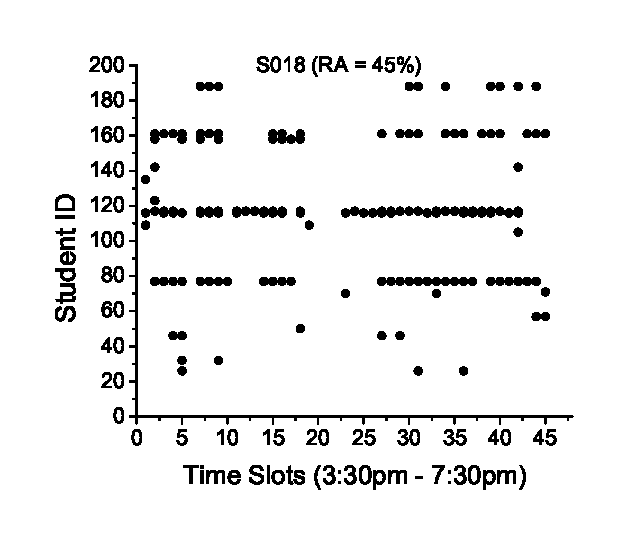
\includegraphics[width=3.5in]{graphs/Figure18.eps}}
\caption{\textit{S018} data on game day with proximity estimation model} 
\label{fig:018_80}
\end{figure}

\begin{figure}[h!tbp]
\centering
{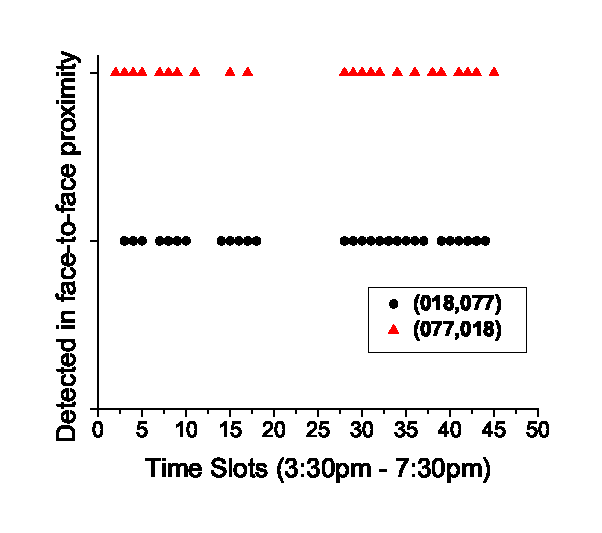
\includegraphics[width=3.5in]{graphs/Figure19.eps}}
\caption{Symmetry analysis of data on game day} 
\label{fig:symmetry}
\end{figure}

\subsubsection{Weekday}
In this part, we analyzed the data recorded during weekdays, such as class time and lunch hours, and compared it with the data on game days. During the football game, most of the freshmen sit in the same student section and it is highly possible to detect more than 10 people around him/her at one time slot. However, when students are in class or having lunch, the data becomes reasonably sparse. Compared to more than fifty thousand records in the game, we recorded 6408 records on Oct 11th 2011 (Tuesday) from 9am to 1pm. Figure~\ref{fig:018_class} illustrates the data reported by the same phone \textit{S018} during this period. Obviously, the chance to meet other students (related to this project) in class or during the lunch time is relatively low. In \textit{S018}'s case, he/she only met with two other students within a direct-communication distance in class and four during the lunch time. 

\begin{figure}[h!tbp]
\centering
{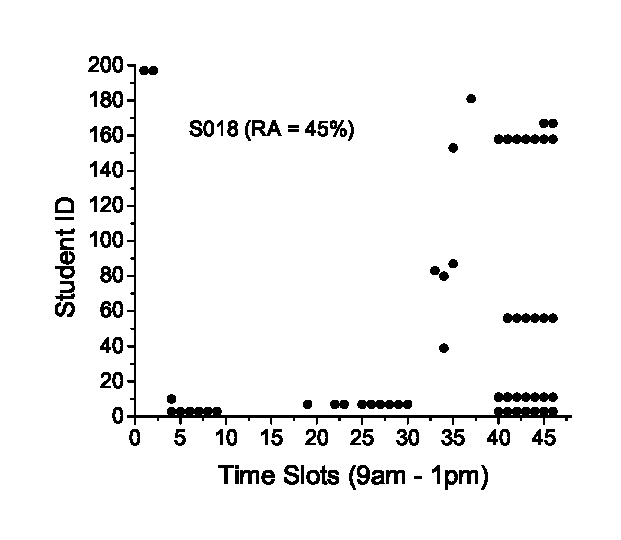
\includegraphics[width=3.5in]{graphs/Figure20.eps}}
\caption{\textit{S018} data on weekday with proximity estimation model} 
\label{fig:018_class}
\end{figure}

\begin{figure}[h!tbp]
\centering
{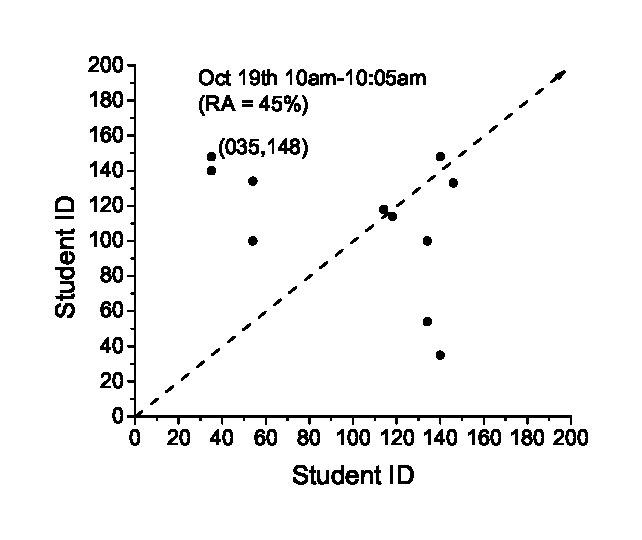
\includegraphics[width=3.5in]{graphs/Figure21.eps}}
\caption{Fallbreak data with proximity estimation model} 
\label{fig:fallbreak}
\end{figure}

\subsubsection{Fall Break}
During the fall break (from Oct 17th to Oct 23rd), most students went home and we got relatively less data. Take the data of Oct 19th for example, we got 4373 records in the whole day and only 26 devices detected other devices in the project in face-to-face proximity. We used the proximity estimation model and the same RA to analyze the results we got on Oct 19th between 10am and 10:05am. Figure~\ref{fig:fallbreak} shows the proximity status among students in this specific time slot. There are in total 11 samples collected during the 5-minutes period and (035, 148) means device \textit{S035} detected \textit{S148} was in the face-to-face proximity. Since there is less interference, the symmetry is maintained as observed in Section~\ref{sec:exp}. In Figure~\ref{fig:fallbreak}, more than 70\% values are symmetric. Compared with self-reporting method, our proximity estimation model is a more reliable and effective method to detect face-to-face proximity in daily life. 

\section{Summary}
In this section, our presented work validates the usage of Bluetooth as a tool for face-to-face proximity detection and makes the following contributions:
\begin{itemize}
\item We demonstrate the viability of using Bluetooth for the purposes of face-to-face proximity estimation and propose a proximity estimation model with appropriate smoothing and consideration of a wide variety of typical environments. 
\item We study the relationship between the value of Bluetooth RSSI and distance based on empirical measurements and compare the results with the theoretical results using the radio propagation model. 
\item Based on the monitoring system, we are able to use the proximity estimation model across several real-world cases to provide high accurate determination of face-to-face interaction distance.
\end{itemize}
Based the empirical Bluetooth RSSI results, we further study the potential of opportunistic relaying when two devices are in close proximity in Chapter~\ref{chap:opp_relay}. 


%
% Chapter 4
%

\chapter{WiFi Offloading}
\label{chap:offloading}

\section{Background}\label{background}
With the advent of the smartphone, mobile data usage has exploded which in turn has created tremendous pressure on cellular data networks.  A promising candidate to reduce the impact of cellular data growth is WiFi offloading. However, our dataset casts doubts on the viability of achieving such 
gains with WiFi offloading. In contrast to the prior work of \cite{lee2010mobile}, we have found that despite users operating in a dense university WiFi environment, the potential gains for the majority of users are quite muted. Rather than finding that WiFi usage dominates 3G usage, our study curiously finds that much of the user consumption of 3G dominates the consumption of WiFi. 

At first glance, such a result would appear to counterintuitive. A dense WiFi deployment\footnote{The
University of Notre Dame was ranked as one of the top 20 wireless campuses in 2010.} would have ample
WiFi access points placed throughout the buildings on the campus. The dormitory-oriented residential
life of the campus meant that all study participants (all of whom were freshmen) would have ubiquitous
WiFi coverage at night (dormitory) as well as during the day (classrooms/dorms). Coverage at the
university is also frequently verified by employing roaming laptops by IT staff throughout campus. However, it is the usage of laptops to validate coverage as opposed to smartphones where the problem
originates.

Consider the observation noted in Table~\ref{table:diff_rssi} that compares the observed RSSI on 
a laptop versus the RSSI observed in the same time period and same location via a representative smartphone 
from the study. In the table, despite being in the same location, the smartphone observes a dramatically
reduced signal strength (around 10dB) versus the laptop. The discrepancy between observed signal strength on the smartphone
is not an isolated phenomenon to one particular smartphone but rather tends to be broadly indicative of many
commercially available smartphones that are subject to marketing and development constraints. This is 
potentially significant for WiFi offloading as most dense WiFi environments (i.e. businesses) tend not 
to be designed at smartphones but rather tend to be designed at laptops.  

\begin{table}[h!tbp] 
\caption{WIFI RSSI ON LAPTOP AND SMARTPHONE} 
\label{table:diff_rssi}
\centering 
\begin{tabular}{|c|c|c|c|c|}
\hline
& \multicolumn{2}{c|}{RSSI on Laptop} & \multicolumn{2}{c|}{RSSI on Smartphone} \\
\hline Access Point & Avg. & Std Dev & Avg. & Std Dev \\
\hline 1 & -75.27 & 2.76 & -83.32 & 2.72  \\ 
\hline 2 & -75.22 & 2.79 & -85.04 & 3.39 \\
\hline 3 & -75.40 & 2.87 & -84.94 & 3.04\\
\hline 4 & -71.99 & 2.06 & -79.52 & 3.51\\
\hline 5 & -72.05 & 2.06 & -80.18 & 3.80\\
\hline 6 & -73.88 & 5.13 & -80.02 & 3.34\\
\hline
\end{tabular}
\end{table}

The period in question analyzed in
this chapter represents eight weeks of continuous data from the end of January 2012 to the end of March of 2012 in the spring semester. The time frame is selected to ensure that the students have fully adapted to 
their phones and represent behaviors typical of their normal phone usage.  The seventh week in the study 
represents spring break (March 10th - March 18th) which offers a likely period where students returned home
for the week. In total, we selected 131 users out of the study (62 female, 69 male) that have continuous data throughout the
entire eight weeks and have more than five minutes per day of usage on the phone. The graphs and tables in this chapter are based on the data collected from these 131 participants. 

\section{Related work}\label{related}
There have been several recent studies proposed to reducing the strain on the overloaded cellular infrastructure with WiFi offloading being one of the main candidate~\cite{balasubramanian2010augmenting,lee2010mobile,dimatteo2011cellular,icc2012performance,han2011mobile}. In~\cite{balasubramanian2010augmenting}, WiFi connectivity is used to reduce the pressure on 3G spectrum when possible for transferring data. In~\cite{lee2010mobile,dimatteo2011cellular,icc2012performance,han2011mobile}, delayed WiFi offloading is introduced to migrate data traffic from cellular networks to WiFi access points. However, such methods are not practical for most access patterns (any interactive app including web browsing and most streaming) as the point of using the smartphone is for data access that moment. Conversely, the de facto solution is upgrading the network to the next generation networks. The configuration details of both WiMAX and LTE technologies are summarized in \cite{khan20094g}. Similarly, \cite{arshad2010evolution} provided an overview of the 4G evolution and categorized how such technologies can accompany a more user focused world of wireless. 

\section{WiFi Offloading in Practice}
Figure~\ref{fig:avg_downlink} shows the average 3G and WiFi downlink traffic per phone per week across the study period. On average, the WiFi traffic takes approximately 30\% of the total data consumption. The average WiFi traffic statistics excludes the data of devices with no WiFi usage. The underlying 802.1X WiFi infrastructure (primarily due to expired passwords) can prevent a user from using any WiFi traffic during that entire week. Once the password is updated (passwords are required to change every 90 days), the phone can correctly use WiFi once again. We note though that an inability to authenticate does not preclude monitoring signal strength (via beacons) and that users do not experience intermittent 802.1X issues (the phones either authenticate or do not contiguously).   

\begin{figure}[h!tbp]
\centering
{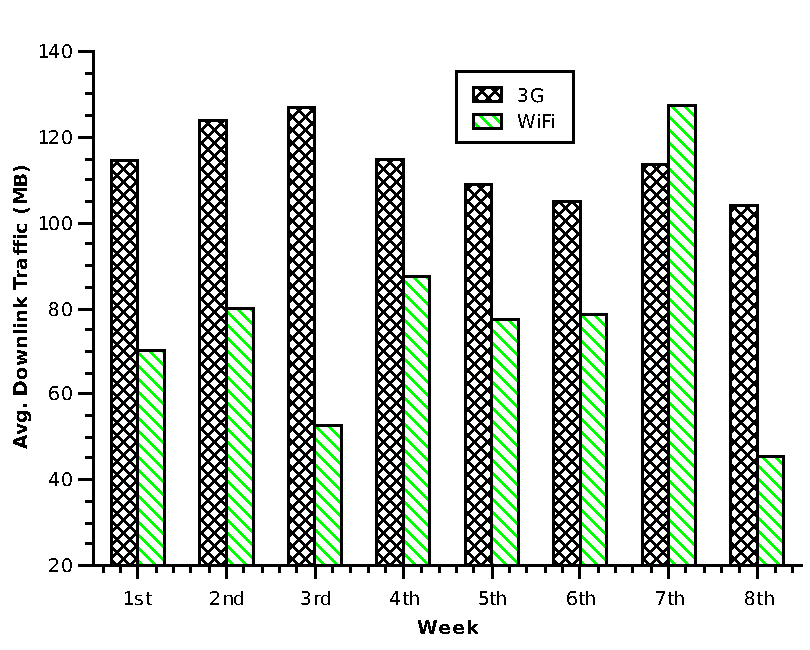
\includegraphics[width = 3.5in]{graphs/avg_downlink2.pdf}}
\caption{Average Downlink Traffic per Phone per Week} 
\label{fig:avg_downlink}
\end{figure}

As noted in Section~\ref{background}, the average WiFi usage is curiously lower than the average 3G usage aside from the week of spring break (likely on a single AP at home) where WiFi barely eclipses 3G usage. In Figure~\ref{fig:switch}, we select a small subset of phones that exhibit a high degree of 3G usage versus WiFi and plot their respective average traffic patterns for a given day during the semester. From 5 PM to 6 PM (1700-1800h), the phones exhibit a degree of asymmetry, favoring 3G over WiFi.  Figure~\ref{fig:weak_wifi_68} explores this time period further noting the detected AP beacons but exceptionally low quality signal strengths over that time period. Hence, the phone naturally defaults to favor 3G over WiFi.  Conversely, during the 10 PM to 11PM (2200-2300h) as noted in Figure \ref{fig:weak_wifi_1012} where the signal strength is better but not great, the ratio between 3G and WiFi changes to favor WiFi over 3G but not markedly so.   

\begin{figure}[h!tbp]
\centering
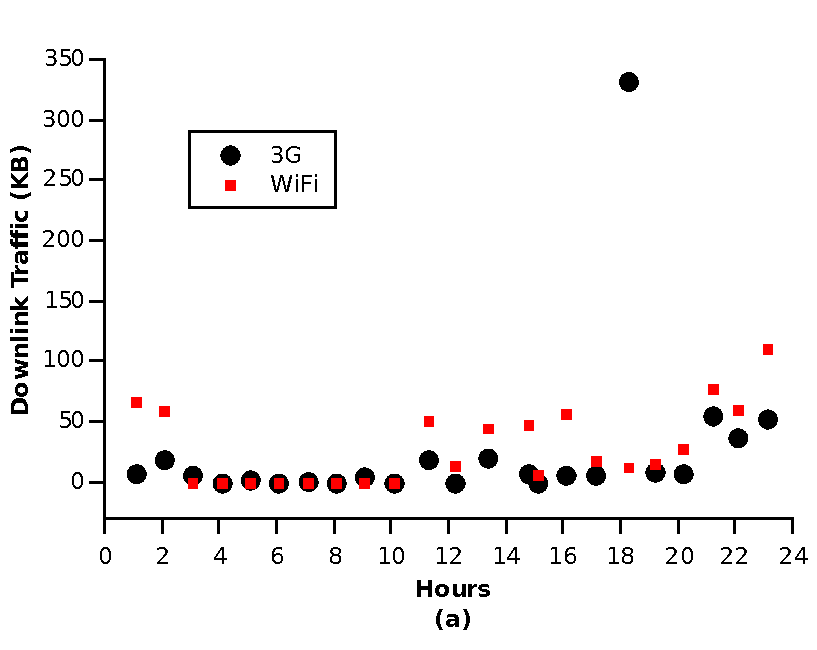
\includegraphics[width = 3.5in]{graphs/traffic_0202.pdf}
\caption{Switch between 3G and WiFi} 
\label{fig:switch}
\end{figure}

\begin{figure}[h!tbp]
\centering
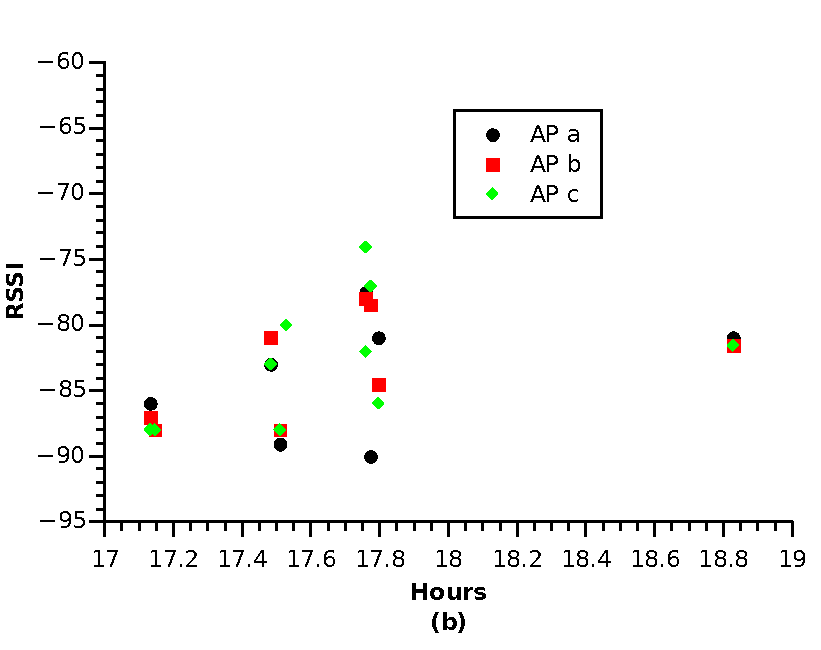
\includegraphics[width = 3.5in]{graphs/weak_wifi_68.pdf}
\caption{WiFi Signal Strength (1700-1800h)} 
\label{fig:weak_wifi_68}
\end{figure}

\begin{figure}[h!tbp]
\centering
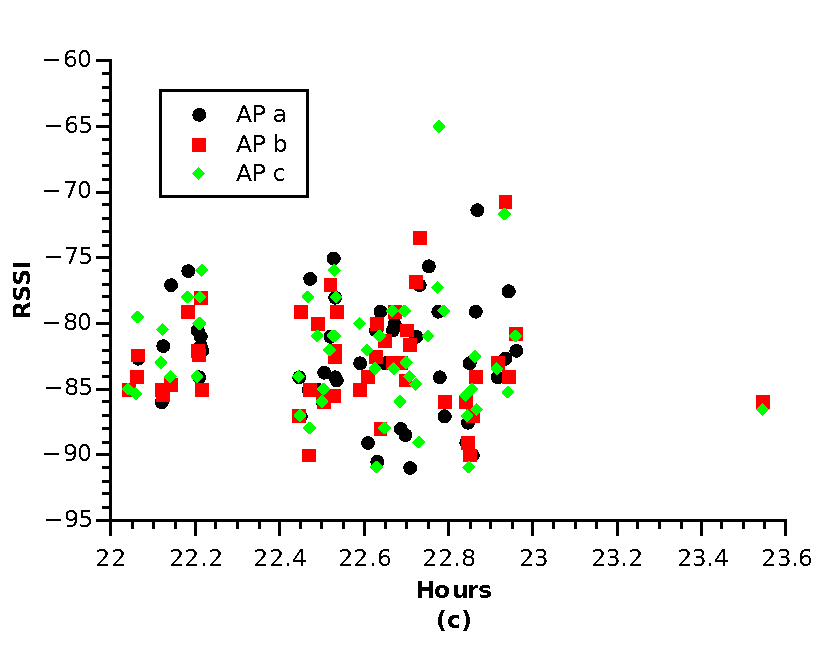
\includegraphics[width = 3.5in]{graphs/weak_wifi_1012.pdf}
\caption{WiFi Signal Strength (2200-2300h)} 
\label{fig:weak_wifi_1012}
\end{figure}

To verify that the users in this subset were indeed active (using the screen), Figure \ref{fig:screen_0202} plots the average screen session lengths over that same selected day. The screen session time captures via event when the screen is turned on (timestamp recorded) and when the screen is turned off (timestamp recorded). While the users were more active in terms of the number of sessions during the later time period (10PM to midnight), the users actually used more data during the earlier time period. We also note that the spike did not correlate with a check in by the agent as such data has been filtered from the results.   

\begin{figure}[h!tbp]
\centering
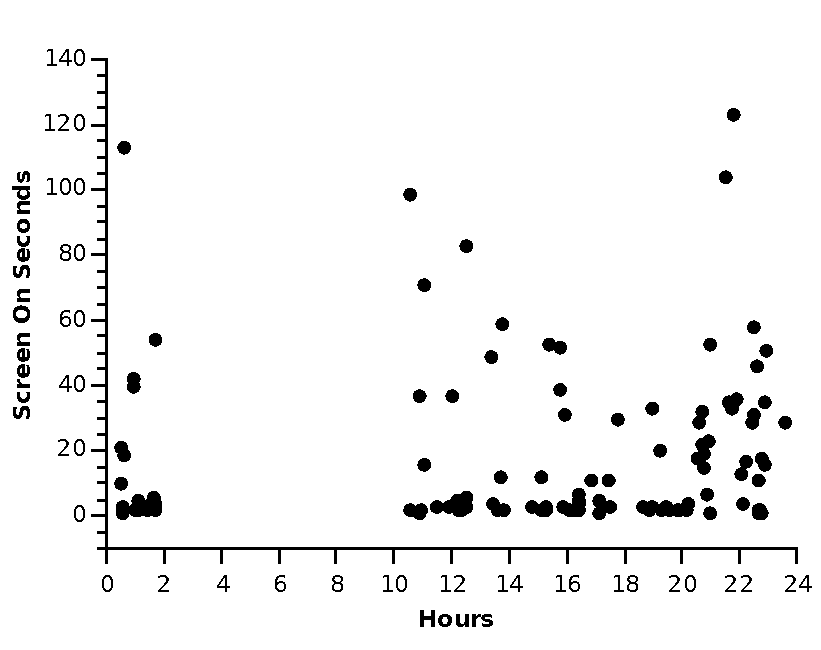
\includegraphics[width = 3in]{graphs/screen_0202.pdf}
\caption{Screen On Duration in One Day} 
\label{fig:screen_0202}
\end{figure}

\section{Comparison of User Behavior}\label{comparison}
We continue our analysis by exploring how user behavior changes if the user is able to get reasonable quantities of 
adequate WiFi smartphone coverage. Figure~\ref{fig:distribution} shows the distribution of the percentage of WiFi downlink
traffic as a ratio versus total traffic for one week (2nd week). The average WiFi consumption ratio is around 30\%. From the figure, we see that there are approximately 30\% of participants whose traffic is offloaded to WiFi for the week by more than 50\%. Conversely, we see that there are 
nearly 20\% of the participants that week who used no WiFi traffic for the reasons mentioned earlier (incorrect password, etc.).

\begin{figure}[h!tbp]
\centering
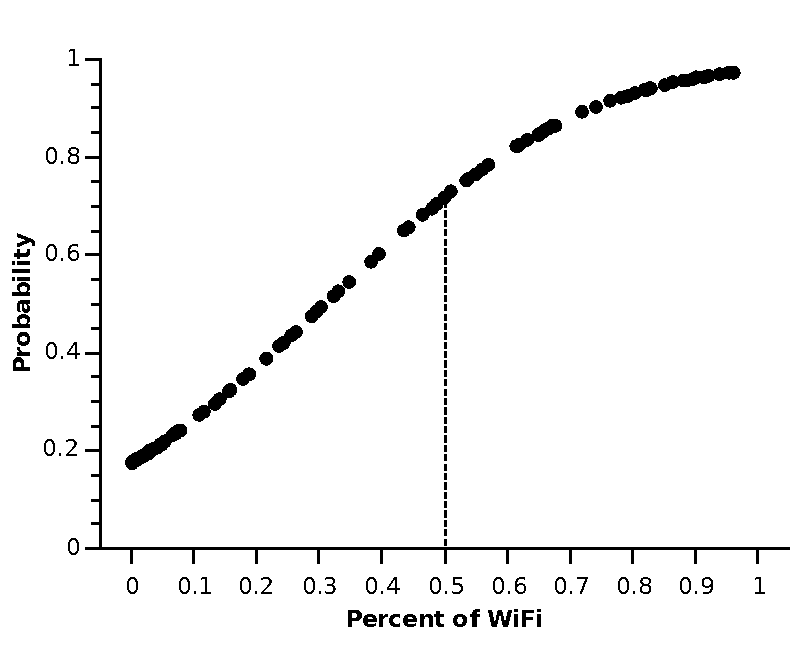
\includegraphics[width = 3.5in]{graphs/distribution.pdf}
\caption{Distribution of Percent of WiFi Traffic} 
\label{fig:distribution}
\end{figure}

For further analysis in the paper, we subdivide the 131 participants into three groups based on their WiFi downlink consumption
ratio versus their total traffic consumption: no WiFi, less than 50\%, and more than 50\%.  We summarize how the participants
break down into each group among the eight weeks in Figure~\ref{fig:number}.  Similarly, the breakdown of males versus females
is shown in Table~\ref{table:gender}. Although the numbers in the  
groups varied, the groups are reasonably well separated to analyze the participants in the various categories.  

\begin{figure}[h!tbp]
\centering
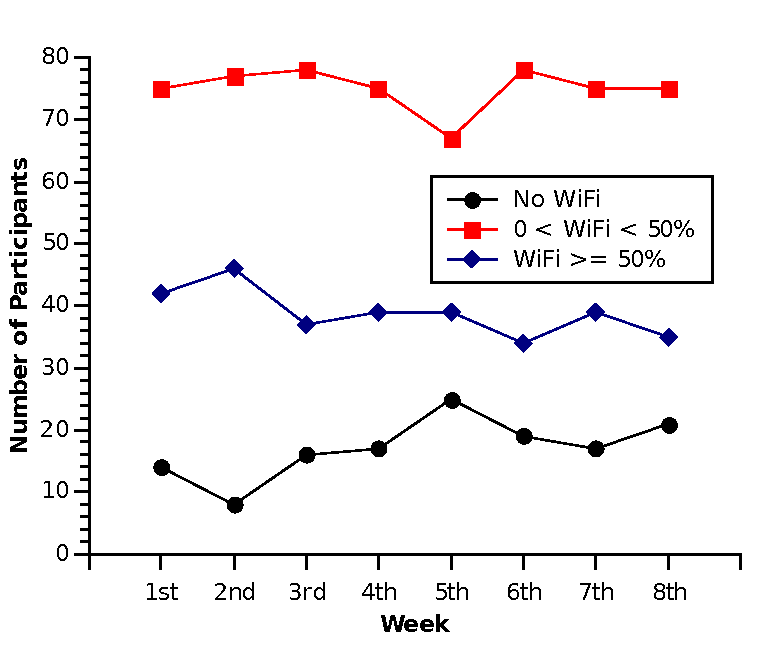
\includegraphics[width = 3.5in]{graphs/number.pdf}
\caption{Numbers of Participant in Groups} 
\label{fig:number}
\end{figure}

\begin{table}[h!tbp] 
\caption{NUMBER OF MALES AND FEMALES IN GROUPS} 
\label{table:gender}
\centering 
\begin{tabular}{|c|cc|cc|cc|}
\hline
Week &  \multicolumn{2}{c}{No WiFi} & \multicolumn{2}{|c|}{0 $<$ WiFi $<$ 50\%} & \multicolumn{2}{c|}{WiFi $>=$ 50\%} \\
\hline
& M & F & M & F &   M & F \\
\hline
 \parbox[t]{3cm}{\hspace{12mm}1st}& 9&5&35&40&25&17\\ 
\hline
2nd &6&2	&35&42&29&17\\
\hline
3rd&5&11&37&41&27&10\\
\hline
4th&7&10&36&39&26&13\\
\hline
5th&15&10&30&37&24&15\\
\hline
6th&9&10&39&39&21&13\\
\hline
7th&8&9&36&39&25	&14\\
\hline
8th&10&11&36&39&23&12\\
\hline
\end{tabular}
\end{table}

Figure~\ref{fig:downlink} shows the average total downlink traffic per phone (3G+WiFi) of the different groups across the eight weeks. For the category of each particular participant, determination was computed on a weekly basis meaning that a user could move between categories. Interestingly enough, we begin to see a growing pattern of separation as the semester goes on and particularly so doing the week of spring 
break. We posit that the week of spring break offered a much more consistent set of WiFi coverage versus what may occur on campus.   

\begin{figure}[h!tbp]
\centering
{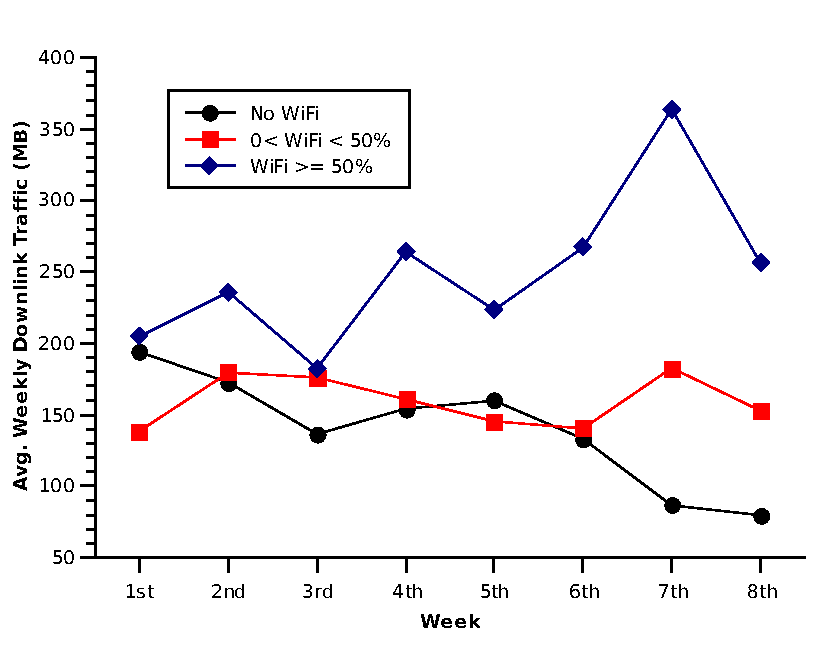
\includegraphics[width = 3.5in]{graphs/downlink.pdf}}
\caption{Weekly Average Total Downlink Traffic per Phone} 
\label{fig:downlink}
\end{figure}

\subsection{Phone Usage}
Related to usage, a secondary question arises with regards to the ratio of screen time to data consumption.  The most straightforward way to indicate whether the person is using the phone is based on the phone screen status (on or off). When the phone screen is on, it is most likely because the person is actively using the phone (sending messages, checking e-mail, playing games, etc.). In order to explore the relationship between phone usage time and traffic usage, we collect the screen on session length on the phones by calculating the duration between screen on and screen off. On average, the screen session lengths vary from 10 seconds to more than 100 seconds. We categorize them into four ranges: (0, 30s), (30s, 60s), (60s, 90s) and more than 90s. Figure~\ref{fig:duration} lists the numbers of participants from three groups in different duration ranges. In the range of (60s, 90s) the number of people who use WiFi more than 50\% is greater than the other two groups numbers. We calculate the weekly total screen on time and the corresponding daily average per phone as well. There are five ranges of daily average from less than half an hour per day to more than 2 hours per day. Figure~\ref{fig:screen} gives an example (data from the 2nd week): compared with purely 3G users (no WiFi), the number of participants who use WiFi more than 50\% in each range is much greater.  The fact that the phone is more useful (faster access) may encourage such additional usage. 

\begin{figure}[h!tbp]
\centering
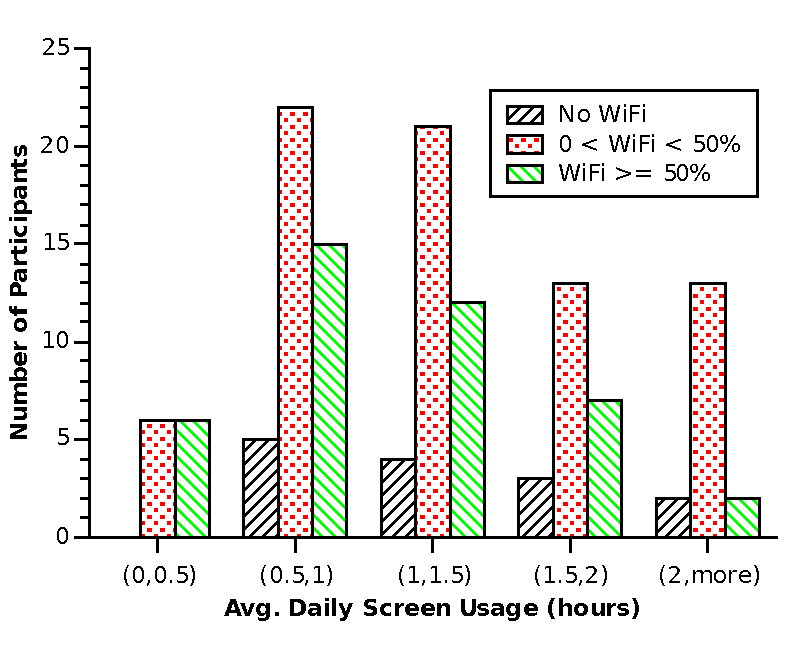
\includegraphics[width = 3.5in]{graphs/screen2.pdf}
\caption{Avg. Daily Screen Usage of Groups} 
\label{fig:screen}
\end{figure}

\begin{figure}[h!tbp]
\centering
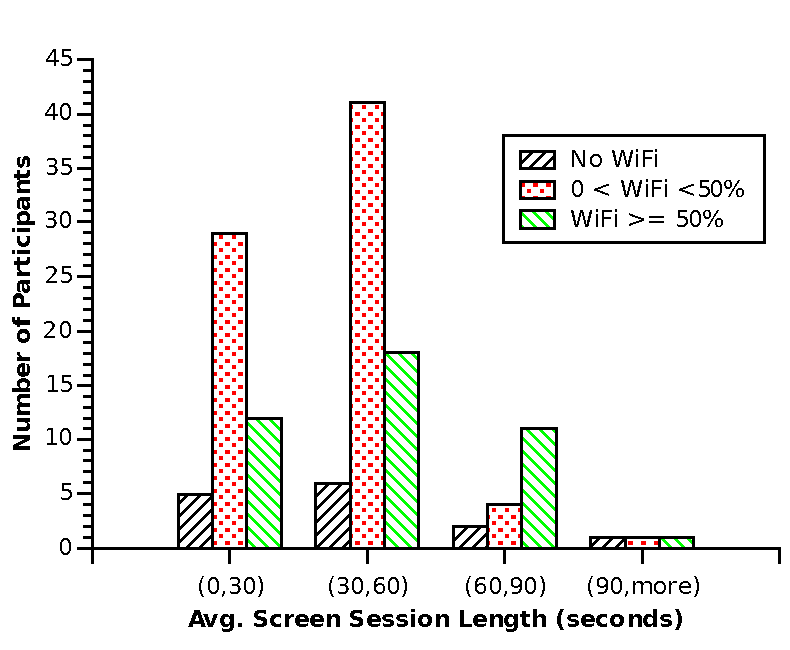
\includegraphics[width = 3.5in]{graphs/duration2.pdf}
\caption{Avg. Screen session length of Groups} 
\label{fig:duration}
\end{figure}

We further calculate the screen session duration across different time slots in a single day to analyze user behavior. As shown in Figure~\ref{fig:dn}, we divide one day into four time slots: morning (7am-12pm), afternoon (12pm-5pm), night (5pm-10pm) and midnight (10pm-7am).  As would
be expected with a student population, usage in the morning is quite low relative to usage in the evening.  

\begin{figure}[h!tbp]
\centering
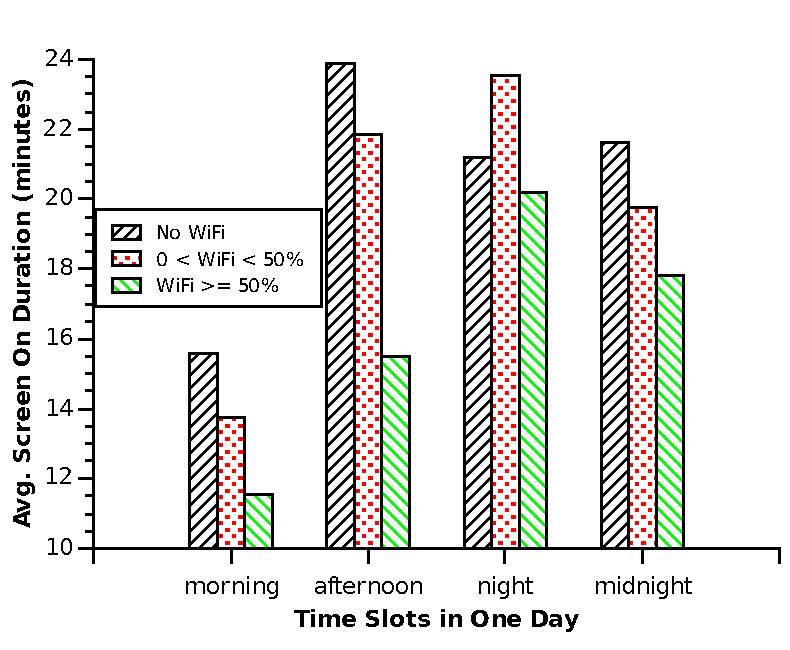
\includegraphics[width = 3.5in]{graphs/dn2.pdf}
\caption{Avg. Screen on Duration in Different Time Slots} 
\label{fig:dn}
\end{figure}

Finally, we explore the relationship of WiFi to 3G usage with respect to various other services on the phone including the number of text
messages, total phone usage, average phone call length, etc. Table~\ref{table:sms_phone} shows the numbers across the entirety of the 
study with users categorized again on a weekly basis.  While WiFi dominant users tended to use their screen for longer
average periods of time, they tended to less frequently use text messages relative to the non-WiFi-dominant users (455 average text messages sent/received per week versus 522 average text messages sent/received per week). Text messages do not count against the data count for either 3G or WiFi usage.  

\begin{table}[h!tbp] 
\caption{WEEKLY SMS/PHONE CALL COMPARISON} 
\label{table:sms_phone}
\centering 
\begin{tabular}{|l|c|c|c|}
\hline
Groups & No WiFi& 0 $<$ WiFi $<$ 50\% & WiFi $>=$ 50\%\\
\hline Avg. Screen On Duration (seconds) & 39.33 & 43.93 & 48.76\\
\hline Avg. SMS All& 436 & 522 & 455  \\ 
\hline Avg. SMS Sent & 209 & 249 & 225 \\
\hline Avg. Number of Phone Calls & 26 & 31 & 24 \\
\hline Avg. Phone Call Duration (hours) & 1.03 & 1.60 & 1.27 \\
\hline Avg. Email All & 89 & 95 & 90\\
\hline Avg. Number of Browser Sessions & 102 & 81 & 67\\
\hline
\end{tabular}
\end{table}

\subsection{App Usage}\label{app}

The network bandwidth and throughput has a profound influence on application usage preference. When the network provides better service,
users tend to use more intensive services.   We look into the data of installed application and application traffic which are logged by the service as part of the agent (hourly application data usage). 

\begin{table}[h!tbp] 
\caption{TOP APPLICATIONS CATEGORIES} 
\label{table:app_categories}
\centering 
\begin{tabular}{|l|c|c|c|}
\hline
& No WiFi & 0 $<$ WiFi $<$ 50\% & WiFi $>=$ 50\%\\
\hline
Top Downlink & Browser & Browser & Netflix\\ 
					& Facebook & Facebook & Browser\\
					& Zynga Words & Pandora & Pandora\\
					& Amazon & Zynga Words & Facebook\\
					& Twitter & Twitter & Dictionary\\
\hline
Top uplink & Google Maps & Google Maps & Pandora\\ 
					& PhoneMonitor & Pandora & Google Maps\\
					& Browser & PhoneMonitor & Glu Games\\
					& Facebook &Browser&PhoneMonitor\\
					& Gmail & Facebook&Browser\\
\hline
\end{tabular}
\end{table}


In Table~\ref{table:app_categories} we summarize the top 5 applications appeared in the each group based on their total downlink or uplink traffic. For the phones using WiFi more than 50\%, streaming apps such as Netflix and Pandora always are the top applications. For the participants using 3G only, their main activities on the phone are web browsing and email checking. Figure~\ref{fig:app_downlink} demonstrates the weekly downlink traffic of the top 10 apps in different categories which include video \& audio (Netflix, Youtube, Pandora and Google Music), social (Facebook and Twitter), tools (Browser, Gmail, Google Maps, Dictionary) and games (Zynga and Glu applications). Similarly, we present the results of uplink traffic in Figure~\ref{fig:app_uplink}. In both graphs, the traffic of video and audio applications increases dramatically when the participants use more WiFi. An interesting
question emerges if the streaming consumption is user specific or rather becomes enabled by WiFi speeds
implying that WiFi with continuous LTE would show the same usage patterns. 

\begin{figure}[h!tbp]
\centering
{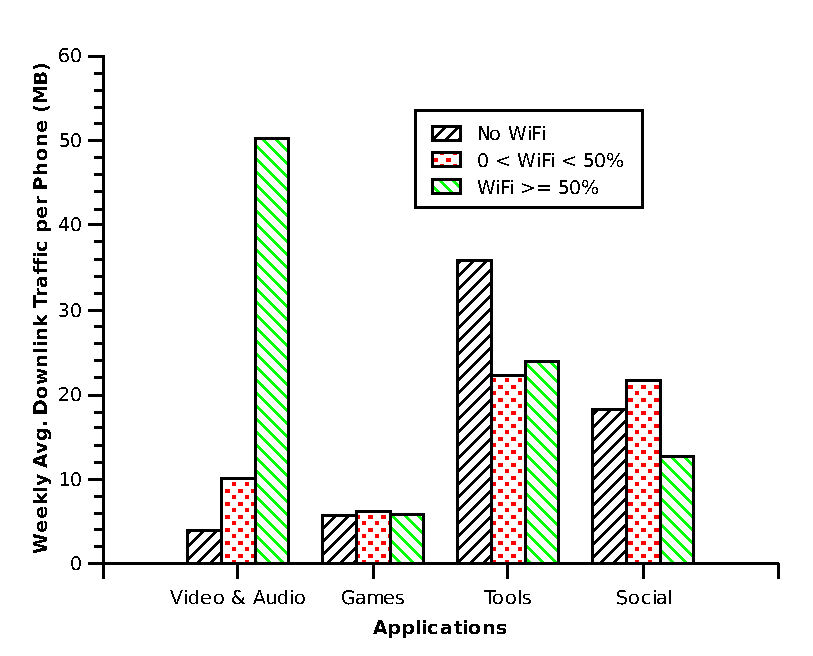
\includegraphics[width = 3.5in]{graphs/app_downlink.pdf}}
\caption{Weekly Application Downlink Traffic} 
\label{fig:app_downlink}
\end{figure}

\begin{figure}[h!tbp]
\centering
{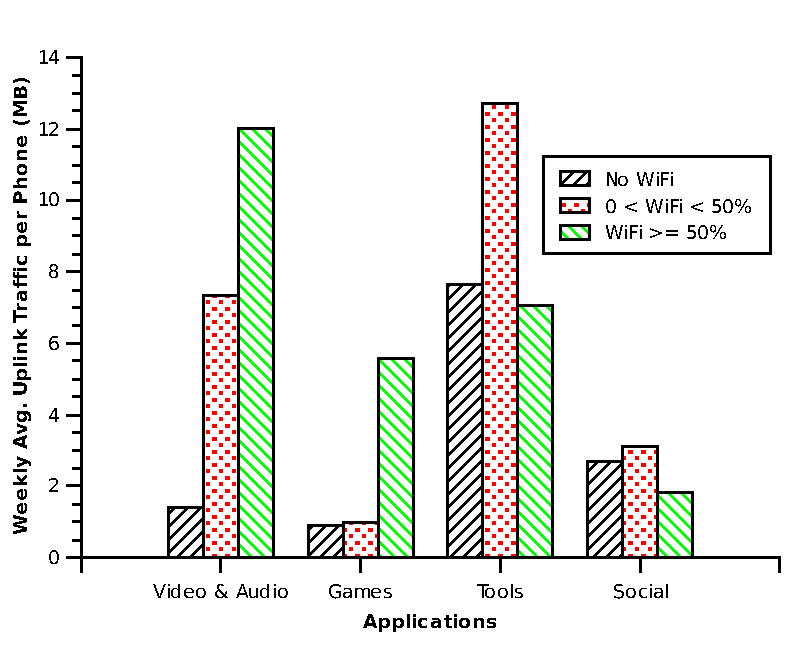
\includegraphics[width = 3.5in]{graphs/app_uplink.pdf}}
\caption{Weekly Application Uplink Traffic} 
\label{fig:app_uplink}
\end{figure}

\section{Summary}
To that end, we make the following contributions in this chapter:
\begin{itemize}
\item The net result of our findings over an eight week period of our smartphone
usage data shows that the gaps in WiFi coverage for smartphones temper the perceived potential gains by 
WiFi offloading. More attention should be paid to WiFi coverage to examine said coverage through the
lens of a typical smartphone rather than a typical laptop or tablet device. 

\item We explore the relationship of WiFi data consumption and phone usage time deduced by screen session length. Moreover,
our work includes accommodations for considering SMS/phone call/browser impacts with regards to phone usage.

\end{itemize}
Although individual handsets (ex. iPhone) may possess better WiFi characteristics, the heterogeneity
of available handsets implies that it is exceptionally likely there will significant variations in the ability of phones to
take advantage of WiFi offloading. While certainly any offloading is desperately appreciated due to capacity
shortages, WiFi offloading may be further clouded by bottlenecks in the next hop following the WiFi link as well. Therefore, we believe that additional scrutiny is needed with respect to the end benefits that can arise from WiFi offloading. In next chapter, we discuss the potential of opportunistic relaying which is complementary to WiFi offloading and demonstrate that the concept of opportunistic networks is powerful in face of data tsunami. 



%
% Chapter 5
%

\chapter{Opportunistic Relaying}
\label{chap:opp_relay}

\section{Background}
Wireless network providers are under tremendous pressure to deliver unprecedented amounts of data to a variety of mobile devices. A powerful concept that has only gained limited traction in practice has been the concept of opportunistic networks whereby nodes opportunistically communicate with each other when in range to augment or overcome existing wireless systems. Although opportunistic networking has received more attention as of late with the rise of various point-to-point technologies (WiFiDirect, LTEDirect) directly embedded in user devices, traction in terms of significant adoption remains elusive as the mere existence of point-to-point wireless technology is insufficient.  Rather, infrastructure support (albeit at a software or protocol level) is still required that is impeded by the lack of shared, longitudinal data taking a serious look at the potential for opportunistic relaying amongst actual mobile device users to justify said investment in infrastructure. The actual gathering of said data though is in and of itself quite difficult, requiring one to overcome numerous issues with respect to privacy, cost, scale, and quite simply the amenability of the device to acquire said data. Thus, in the absence of real data and the difficulty in acquiring such data, opportunistic networking research has largely espoused synthetic or theoretical explorations of user mobility.  In this Chapter, we demystify the opportunities that exist for opportunistic relaying by bridging the gap with our large scale dataset. 

\section{Related Work}\label{sec:related_work}
The notion of what constitutes an \emph{opportunistic communication} encompasses a wide variety of research and standardization efforts within the networking community.  From the more traditional perspective, opportunistic relaying represents wireless nodes taking advantage of emergent opportunities to relay data towards its eventual destination originally espoused by~\cite{laneman2004cooperative} and expanded up by numerous others \cite{bletsas2006simple,lu2009design,bahl2009opportunistic}.  More recently, considerable efforts have emerged where IEEE 802.11-based networks (WiFi) are viewed through an opportunistic viewpoint, espousing the delay of packets to favor the potentially faster WiFi over the congested cellular link.  More aggressive variants include `Opp-Off' as proposed in~\cite{han2011mobile2} which intentionally delays the delivery of information over cellular networks and offload it through the `free' opportunistic communications. Similarly, in~\cite{dimatteo2011cellular}, another delay-tolerant network (DTN)-like architecture called `MADNet' is proposed by integrating WiFi networks and mobile-to-mobile Pocket Switched Networks (PSN) with cellular networks.   With the ability to leverage the availability of inexpensive 802.11, both Opp-Off and MADNet are able to conduct real-world experiments on live systems, albeit on a limited scale and time period.   

A key foundation for the evaluation of opportunistic networks arises from the characterization of inter-contact times 
~\cite{chaintreau2007impact,cai2008toward,lee2009slaw,karagiannis2010power,passarella2011characterising}. The work in \cite{chaintreau2007impact} was one of the first works to highlight the importance of inter-contact for studying opportunistic networks and analyze the features of aggregate inter-contact times. In the work of~\cite{cai2008toward,lee2009slaw}, the mobility models proposed for opportunistic networks aim at reproducing the aggregate power-law distributions.  The mobility models in turn provide powerful abstractions for the evaluation of various theoretical properties of opportunstic networks that is critical for understanding general limits of the overarching relay protocols.  In contrast from these studies on statistical patterns of human mobility, we focus on the analysis to take in not only the proximity into consideration but also other elements such as traffic needs and battery influences which have to the best of our knowledge, not explored in a unified manner in the literature. 

\section{Evaluating Practical Relaying}\label{sec:potential}

The dataset outlined in Chapter~\ref{chap:dataset} provides a fascinating opportunity to evaluate the actual prevalence with respect to opportunistic relaying in the `wild' evaluating not only the prevalence itself but when intra-study proximity is involved, significant explorations with respect to the mutual benefits of relaying or collaborative efforts.  For the purposes of evaluation, we are concerned with two types of opportunistic networking, namely relaying and collaboration.  In the first case of relaying, a mobile node ($MN_i$) might relay the traffic from mobile node ($MN_j$) when $MN_j$ has a weak / non-existent wireless signal or $MN_i$ has a good signal to a preferred wireless medium (ex. WiFi) while $MN_j$ does not.  In the second case of collaboration, $MN_i$ and $MN_j$ work together to overcome a lossy channel either by the use of striping across both nodes (ex. auxiliary relaying of TCP ACKs \cite{SteenkisteRelayACK}) or striping across different wireless mediums (WiFi + cellular).  Opportunistic communications would be provided through mobile-to-mobile communications (Bluetooth, WiFiDirect, LTEDirect). Both approaches to opportunistic relaying would require modifications to the wireless infrastructure as well as security concerns to establish any mobile-to-mobile communication which are beyond the scope of this paper.  Rather, we focus on the more fundamental question of \emph{does enough opportunity exist} and if so, \emph{is it of reasonable quality to make it worthwhile}?  

\begin{landscape}
\begin{table*}[t] 
\caption{FRAMEWORK FOR EVALUATING AVAILABILITY, PREVALENCE, STABILITY, RECIPROCITY} 
\centering
\begin{tabular}{l|p{3.5cm}|p{1.5cm}|p{11cm}}
\hline
\multicolumn{2}{c|}{Criteria} & \multicolumn{1}{c|}{Term} &\multicolumn{1}{c}{Description}  \\ 				
\hline
\hline  
\multirow{5}{*}{Availability}   & Sufficient Signal & $SS$ 	& `good signal' to indicate proximity  \\ 
\cline{2-4}		 			  & Symmetry & $Sym$		& Time when proximity is symmetric, has $SS$ vs. time powered on \\
\cline{2-4}		  		           & Diversity & $Div_n$	         & Time with at least $n$ nodes with $SS$ detected vs. time nodes detected \\ 
\cline{2-4}					  & Residual Battery & $RB$	& Time with proximity of other nodes with $SS$ and enough battery to do relaying vs. time with proximity \\

\hline  
\multirow{2}{*}{Prevalence}   & Time in Proximity & $TIP$ 	& Time with proximity vs. time powered on  \\ 
\cline{2-4}					  & Intercontact Time & $IT$	& Time between two successive contact/proximity periods \\
\cline{2-4}					  & Effective Utility & $EU$	& Time with proximity of other nodes with $SS$, $Sym$, traffic to send vs. time with traffic to send \\

\hline \multirow{4}{*}{Stability} 		& Duration & $D$			& Number of consecutive contact durations vs. instances of contact at $MN_i$ \\
\cline{2-4}			     			&  Node Strength & $NS$	&  Number of total appearances by $n$ most common peers \\
\cline{2-4}			     			&  Total Appearances & $TA$	& Number of appearances of a device vs. total device appearances at $MN_i$ \\
\cline{2-4}			     			&  Continuous Appearances & $CA$	& Number of consecutive appearances of a device vs. appearances of multiple days at $MN_i$ \\
\hline \multirow{4}{*}{Reciprocity}  & Need Service & $Serv$ & Time when no auxiliary WiFi is present and traffic demand exists vs. time powered on\\
\cline{2-4}	  		       		 & Offer Assistance & $Assist$ & Time ween detected with $SS$ vs. time powered on 	\\
\cline{2-4}					 & Ratio Need vs. Assist & $R_{NA}$ & Time of $Serv$ vs. Time of $Assist$ \\ 
\hline
\end{tabular}
\label{table:metrics} 
\end{table*}
\end{landscape}

To that end, we seek to answer the following questions in this section of the paper summarized in terms of metrics in Table \ref{table:metrics}:

\begin{itemize}
	\item \emph{Availability}: How is proximity defined and what criterion should exist to enable opportunistic communication with respect to inter-node communications?  What can be considered a `good' opportunistic link in terms of the underlying physical link quality and at what granularity is such data recorded? How does the residual battery influence the potential for relaying? 
	\item \emph{Prevalence}: What is the frequency that a mobile device detect other devices in proximity?  To what extent is the detection symmetric for intra-study participants?  How does the inter-contact times of nodes compare to prior work?  Do opportunities exist when needed (traffic demand) making them useful versus simply available?  
	\item \emph{Stability}: To what extent are discovered opportunities stable enough that an overarching security mechanism could complete or relevant data exchanges could take place?  Are there consistent patterns with regards to nodes appearing more common than others allowing expedited trust?   
	\item \emph{Reciprocity}: Even if opportunities are shown to be prevalent and stable, to what extent are the relationships likely to be reciprocal, namely both $MN_i$ and $MN_j$ will benefit on average equally in terms of both receiving assistance and giving assistance?  When energy is factored in as a consideration for nodes not being willing participants, does any sort of prevalence or reciprocality disappear?  Finally, reciprocality if it exists, does it exist exclusively in only longer-time scales or does it exist on reasonably short-time scales as well?    
\end{itemize}

For the wireless network, we first being by defining several key attributes of the data.  Each mobile node ($MN_i$) is considered to have a discrete set of samples at periodic intervals capturing the proximity of nearby nodes (Bluetooth), the signal strength from each detected Bluetooth node as received at $MN_i$, (ex. $MN_j \rightarrow MN_i$), each detected AP and also the signal strength for each AP as detected by $MN_i$ by virtue of the beacon signal strength.  Each time slot is assumed to be five minutes long (for the purposes of assessing if the phone was on or off) though durations of contact are calculated using per-minute measurements.  The term \emph{Good RSSI} refers to thresholds for RSSI values that indicate the potential for excellent performance although in practice such performance may vary.  Performance with respect to each node is normalized unless explicitly noted to the actual time that the phone was on (powered on, agent running) for that particular day or period. 

\subsection{Availability}
The first question to pose is how to define proximity. We begin with the most basic question with regards to the signal strength of discoverable Bluetooth devices and detected APs and further refine our queries to explore various aspects of availability through the Availability criterion of the APSR framework. 

\subsubsection{Proximity}
As demonstrated in Chapter~\ref{bt_proximity}, we use Bluetooth as the proximity mechanism for multiple reasons.  First, the effective range of Bluetooth typically is on the order of 10m or less.  In contrast with other point-to-point technologies such as WiFiDirect and LTEDirect which have the potential for significantly longer ranges, Bluetooth in effect represents a minimum or floor to the potential for opportunistic communications as the various *Direct technologies would easily be able to cover the 10m effective range of Bluetooth.  Second, although Bluetooth is reasonably common amongst smart phones, the locking of a device as being discoverable is fairly uncommon, largely for reasons of security.  Despite the somewhat uncommon nature of discoverable Bluetooth (most devices require specific action to make themselves discoverable), a robust finding even with the limits of Bluetooth discoverability represents again a floor or minimum potential available.  Critically, the act of gathering Bluetooth discoverable devices is reasonably power efficient allowing one to gather available devices at a reasonable pace (with associated signal strength for Bluetooth) without pairing and while still having a reasonable device battery life for the study. 

Notably, the mere existence of the device being discoverable does not necessarily imply that the point-to-point link will be suitable for opportunistic communications.  Figure~\ref{fig:rssi} shows the ECDF of the Bluetooth RSSI values in different months and more than 60\% of the values are larger than -80dBm.  In particular, the data of July 2012 consider all the records including the Bluetooth devices outside the project and APs not under university control. Based on the work in ~\cite{polastre2005telos}, the RSSI value \emph{-80dBm} is used as a threshold to indicate good Bluetooth RSSI for direct mobile-to-mobile communication.  

\begin{figure}[tbp]
\centering 
{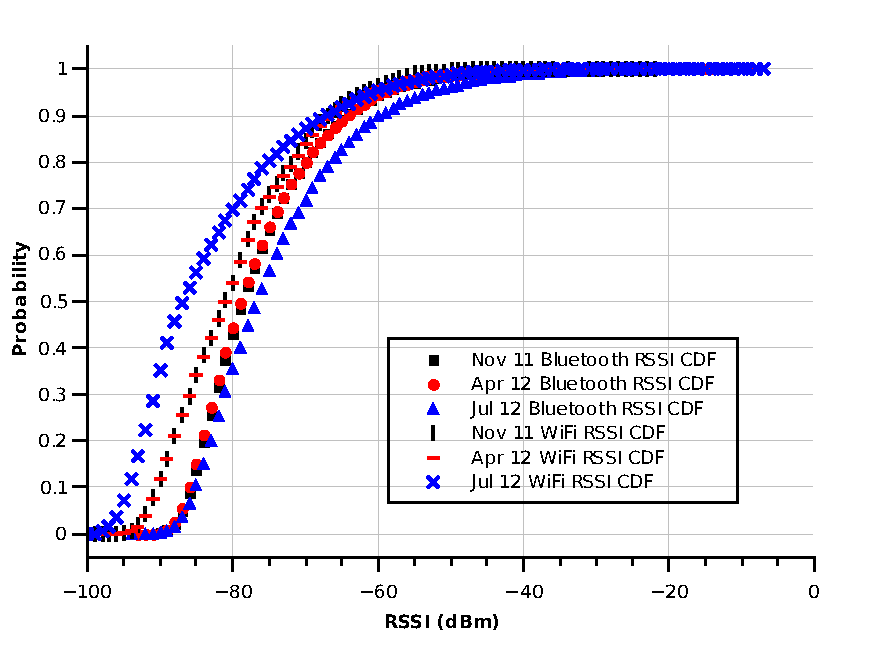
\includegraphics[width=3.5in]{graphs/rssi.pdf}}
\caption{Bluetooth and WiFi RSSI Values ECDF} 
\label{fig:rssi}
\end{figure} 

While Bluetooth is used in the first part of the section to assess proximity, to what extent could we infer proximity if we expanded our search to consider common detected WiFi APs.  For instance, in ~\cite{mcnett2005access}, WiFi signal strength is used to indicate proximity when two devices are associated to the same AP.  We further restrict the characterization to infer proximity if two mobile nodes detect two or more same access points.  Barring the two APs being situated nearly on top of one another (note that university APs are filtered down to disambiguate virtual APs), one can reasonably infer that two nodes sharing the same two or more APs could be in WiFiDirect and / or LTEDirect range. Figure~\ref{fig:bt_wifi_distribution} shows the ECDF of Bluetooth proximity percentage and WiFi proximity percentage. The percentage of time represents the percentage of time where an opportunity might exist for collaboration either within Bluetooth proximity or WiFi proximity. Interestingly, the WiFi result conveys less proximity than the noted Bluetooth proximity.  The discrepancy can be traced to one primary culprit, namely the poor signal reception of smartphone WiFi adapters as originally noted by \cite{liu:CellNet12}.  Notably when compared to reference laptops or tablets, the work in \cite{liu:CellNet12} notes a roughly 10 dBm signal penalty for the smartphone.  The net result is in addition to the detection of WiFi APs being hampered, reasonable placement of APs and auto-tuning of AP strength would result in significantly reduced probabilities of multiple mobile devices being able to detect one or more APs. In Figure~\ref{fig:wifi_fp_fn0}, we compare the results of WiFi proximity and Bluetooth proximity in April of 2012 and November of 2011. The false positive means the device detects other(s) in WiFi proximity which are not detected by Bluetooth proximity. On the other hand, the false negative means that the device does not detect some device in WiFi proximity but does detect the device in Bluetooth proximity. Notably, the false positive in the context of WiFi may not be a false positive but the false negative most certainly represents an incorrect result due to the aforementioned signal holes noted in \cite{liu:CellNet12}.  

\begin{figure}[tbp]
\centering 
{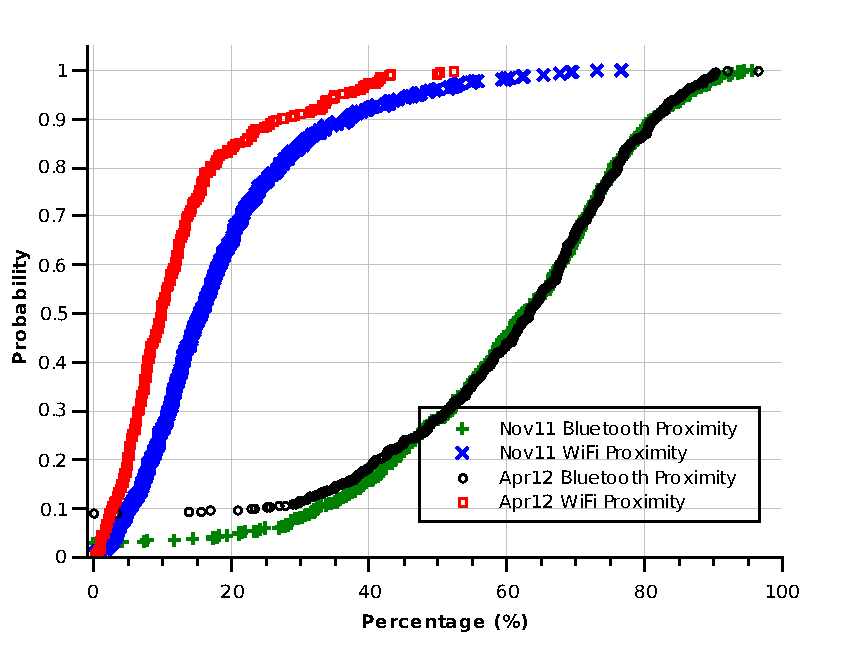
\includegraphics[width=3.5in]{graphs/bt_wifi_distribution_201204.pdf}}
\caption{Bluetooth Proximity and WiFi Proximity ECDF in April 2012} 
\label{fig:bt_wifi_distribution}
\end{figure} 

\begin{figure}[tbp]
\centering 
{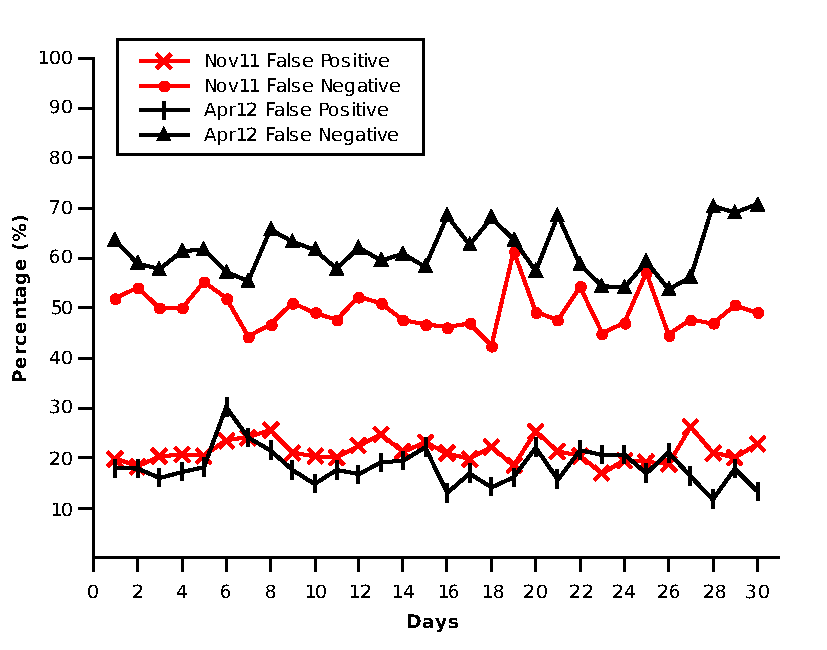
\includegraphics[width=3.5in]{graphs/wifi_falsenegative.pdf}}
\caption{Comparison of Bluetooth Proximity and WiFi Proximity} 
\label{fig:wifi_fp_fn0}
\end{figure} 

\subsubsection{Symmetry}

Symmetry is defined as both nodes seeing each other in proximity. For WiFi proximity, such symmetry is 100\% based on its definition. However, for any two study participants in Bluetooth proximity, there exists the opportunity to determine if detection symmetric exists, namely do both nodes detect each other and even if both nodes detect each other, do both nodes have a `Good RSSI' to one another ($MN_i \rightarrow MN_j$ and vice versa)? In Figure~\ref{fig:daily_symmetric}, the symmetry of Bluetooth proximity within study with `Good RSSI' is illustrated by using the data in November 2011 and April 2012. Notably, roughly one third of the opportunities disappear due to the consideration of symmetry. Many reasons may cause the asymmetry such as environment inference and it is quite expectable in practice. 

\begin{figure}[tbp]
\centering 
{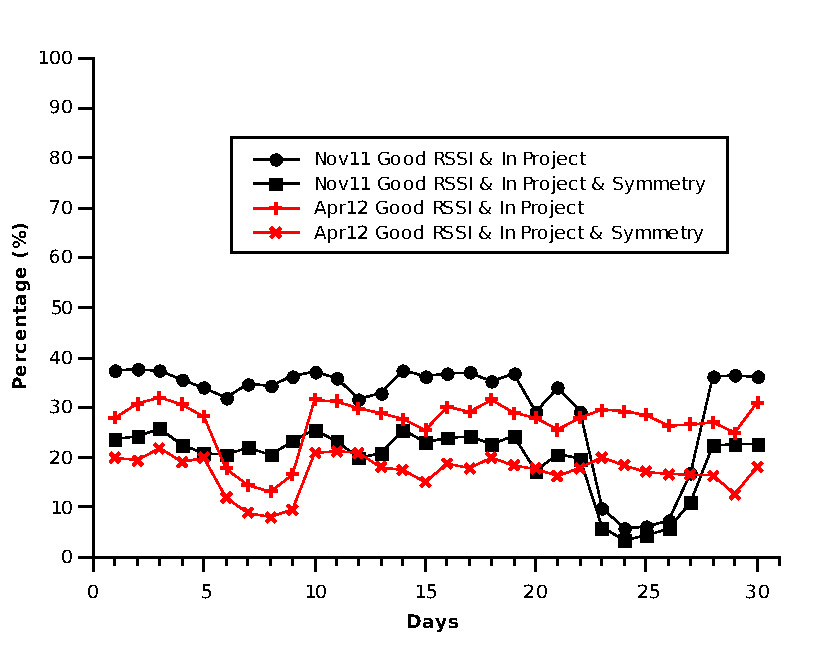
\includegraphics[width=3.5in]{graphs/daily_symmetric.pdf}}
\caption{Symmetry of Bluetooth Proximity} 
\label{fig:daily_symmetric}
\end{figure} 


\subsubsection{Diversity}
While symmetry represents just one part of the puzzle, an related factor for the opportunity to be useful is with regards to the diversity of opportunities available.  Relaying selection plays little role when there exists only a single device to choose from for relaying.   Figure~\ref{fig:relay_num} shows the breakdown of detected devices in proximity through both Bluetooth and WiFi in April 2012 representing only cases where proximity occurred. In the figure, nearly 60\% of time has only one peer is detected among all the possible opportunistic time slots. Meanwhile, there is nearly 20\% of the time when two opportunities are detected and finally 20\% when three or more opportunities are detected. In Figure~\ref{fig:relay_num_diurnal}, more details about the number of detected devices in April 2012 is illustrated with a diurnal distribution across the same month breaking down only cases where proximity was detected, i.e. 50\% of daytime detections involved only a single device in the study. During the daytime, the chance to detect two or more devices in proximity is higher than other durations. Again, day time offers an increased potential for diversity in large part due to the increased mobility around the campus.  

\begin{figure}[tbp]
\centering 
{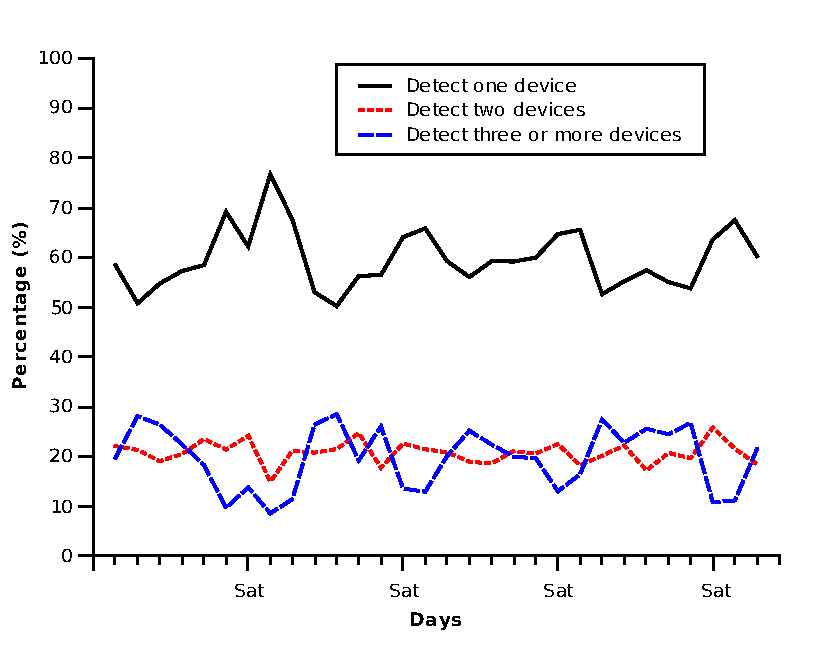
\includegraphics[width=3.5in]{graphs/relay_num.pdf}}
\caption{Distribution of Proximity Diversity (In-Study) in April 2012} 
\label{fig:relay_num}
\end{figure} 

\begin{figure}[tbp]
\centering 
{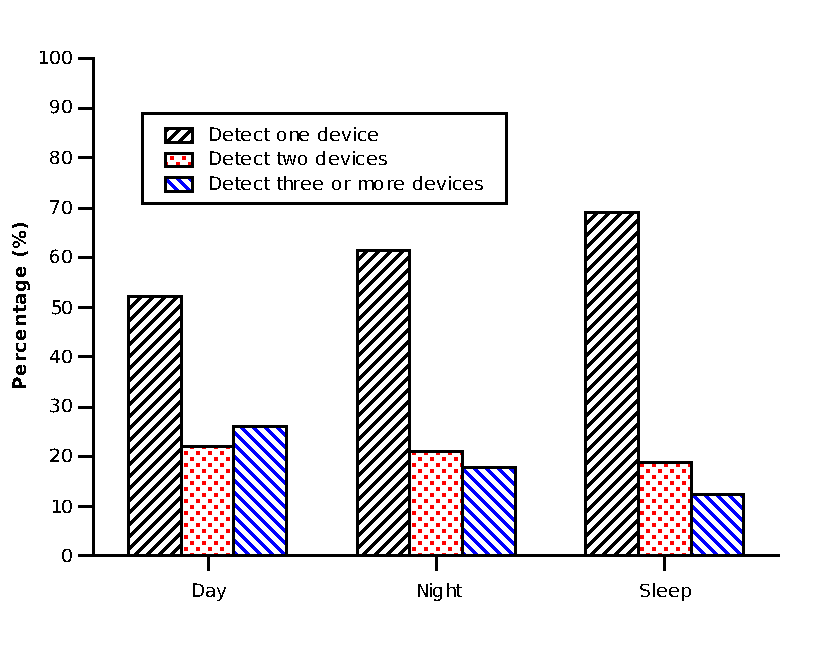
\includegraphics[width=3.5in]{graphs/relay_num_diurnal.pdf}}
\caption{Diurnal Distribution of Proximity Diversity in April 2012} 
\label{fig:relay_num_diurnal}
\end{figure} 

As mentioned before, it is fairly uncommon making the device Bluetooth discoverable. In order to reveal the diversity of potential relaying nodes, we investigate the types of available Bluetooth devices in proximity based on the Bluetooth data across the study. There are around 49\% of distinguished Bluetooth discoverable devices are smartphones. Interestingly, 10\% of the devices are Apple products: 80\% of them are iPhone/iPod/iPad, and rest of them are Macbook laptops. 

\subsubsection{Residual Battery}
The availability of opportunistic communication depends on not only the existence of devices in proximity, but also the battery status of detected devices, i.e. making sure the relaying devices have enough residual battery for the following communication. As discussed in~\cite{zou2012exploiting, madan2008energy}, residual battery is an important consideration factor for relaying selection. Even the device is detected in proximity, it cannot be utilized for relaying if the battery is too low to do transmission. At the same time, it is the basic premise for device having enough energy for communication when it detects other devices in proximity. 
Due to the battery data collection limitation, we focused on the devices within the project and analyzed the percentage of Bluetooth proximity when the battery level is low (i.e. level value smaller than 30) and the result is shown in Figure~\ref{fig:battery}. In April 2012, daily power on time is around 18 hours on average and the low battery time when the devices are in proximity scenarios is nearly 1 hour. Meanwhile, the average time of detecting proximity and being detected as proximity is around 7 and 5 hours. Therefore, the percentage of low battery time is relatively small and 

\begin{figure}[tbp]
\centering 
{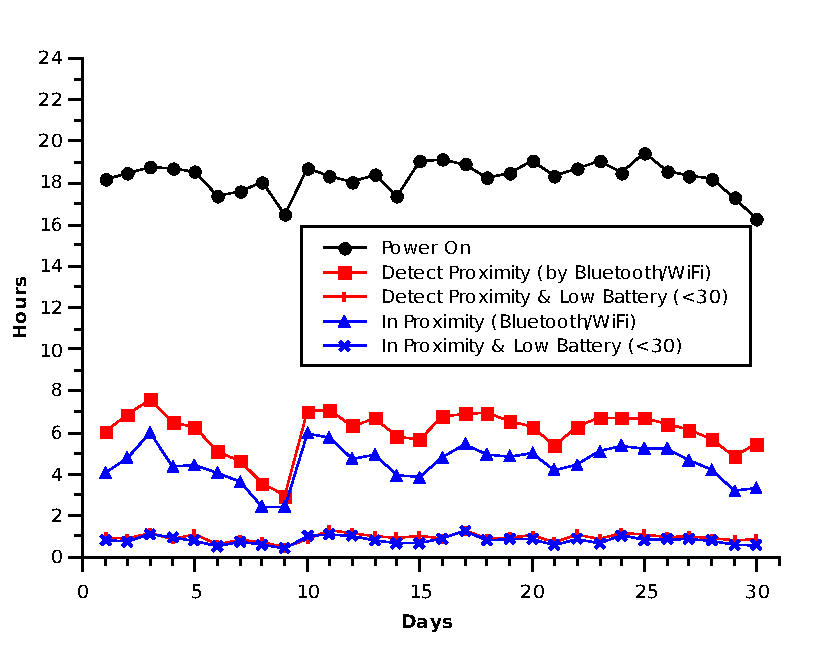
\includegraphics[width=3.5in]{graphs/battery.pdf}}
\caption{Average Daily Low Residual Battery Time in April 2012} 
\label{fig:battery}
\end{figure} 

\subsubsection{Evaluating Availability} 

To summarize, we conclude availability of opportunistic communication with a brief discussion of metrics used to evaluate availability.
\begin{itemize}
	\item Sufficient Signal: While the use of all available proximity potentially may be of interest, only useable mobile-to-mobile links are of interest.  An explicit filter likely unique to each particular handset or device should be employed.  
	\item Symmetry: Filtering the data further, agents monitoring the signal strength on both sides of the dyadic pair can assess if symmetry exists both with respect to detection ($MN_i$ detects $MN_j$, vice versa) and sufficient signal strength.  
	\item Diversity: When there are more than one relaying nodes nearby, it is easier for the device to choose one of the most appropriate nodes with the consideration of benefits on both sides. 
	\item Residual Battery: As an important criterion for relaying selection in various relaying protocol, battery of mobile devices is essential for availability. When the residual battery of mobile devices is low, it is difficult for the devices to do opportunistic communication.  
\end{itemize} 

\subsection{Prevalence}\label{sec:prevalence}
Availability analysis exhibits the possibility to detect other devices in proximity. A more important question is to what extent such opportunistic communication opportunities exist in practice.  We begin with the most basic question with regards to the prevalence of discoverable Bluetooth devices and further refine our queries to explore various aspects of prevalence through the Prevalence criterion of the APSR framework.  We posit several questions that include: (1) the extent to which discoverable Bluetooth devices exist, (2) the extent to which WiFi proximity exist, (3) and the extent to which diurnal (daily) patterns play a role in discoverable devices.  We further continue the explorations examining the prevalence of proximity to determine if the prevalence of such opportunities are still useful, namely (1) are such opportunities only available when there is no traffic and (2) how frequent do opportunities exist to augment access to `better' wireless channels (ex. WiFi).   

\subsubsection{Time in Proximity}
Based on the 15 months data, Figure~\ref{fig:bluetooth} illustrates the average weekly Bluetooth proximity percentage with different restrictions across the study period.  Various periods of interest representing various break periods are labeled in the graph. Further restrictions are placed on the data to filter for `good RSSI' and candidates for opportunistic communications to exist only within the project (study).   Notably, when completely unrestricted opportunities exist on the average of nearly 60\% of the time when on campus, falling only slightly when good signal strength is added as a restriction.  Even intra-study opportunities are quite prolific despite the fact that the 200 study participants represent less than one tenth of the freshmen class and less than 2.5\% of the overall university student population.With the threshold of -80dBm for the `Good RSSI', there still exists more than 50\% of the time slots, a fairly insubstantial drop from the raw detected Bluetooth devices. The slight drop from the fall of 2011 to the fall of 2012 can largely be attributed to students joining their respective majors and having less shared coursework versus their freshmen year.  Moreover, we compare Bluetooth proximity with and without consideration of symmetry. Similarly as the results in Figure~\ref{fig:daily_symmetric}, the one third drop rate due to asymmetry is quite stable across the study.  Although the lack of symmetry does temper the earlier findings of prevalence, we note that Bluetooth is most appropriately viewed as a floor for potential interactions.  The potential for asymmetry though between nodes does represent a consideration that merits further attention.  

\begin{figure}[tbp]
\centering 
{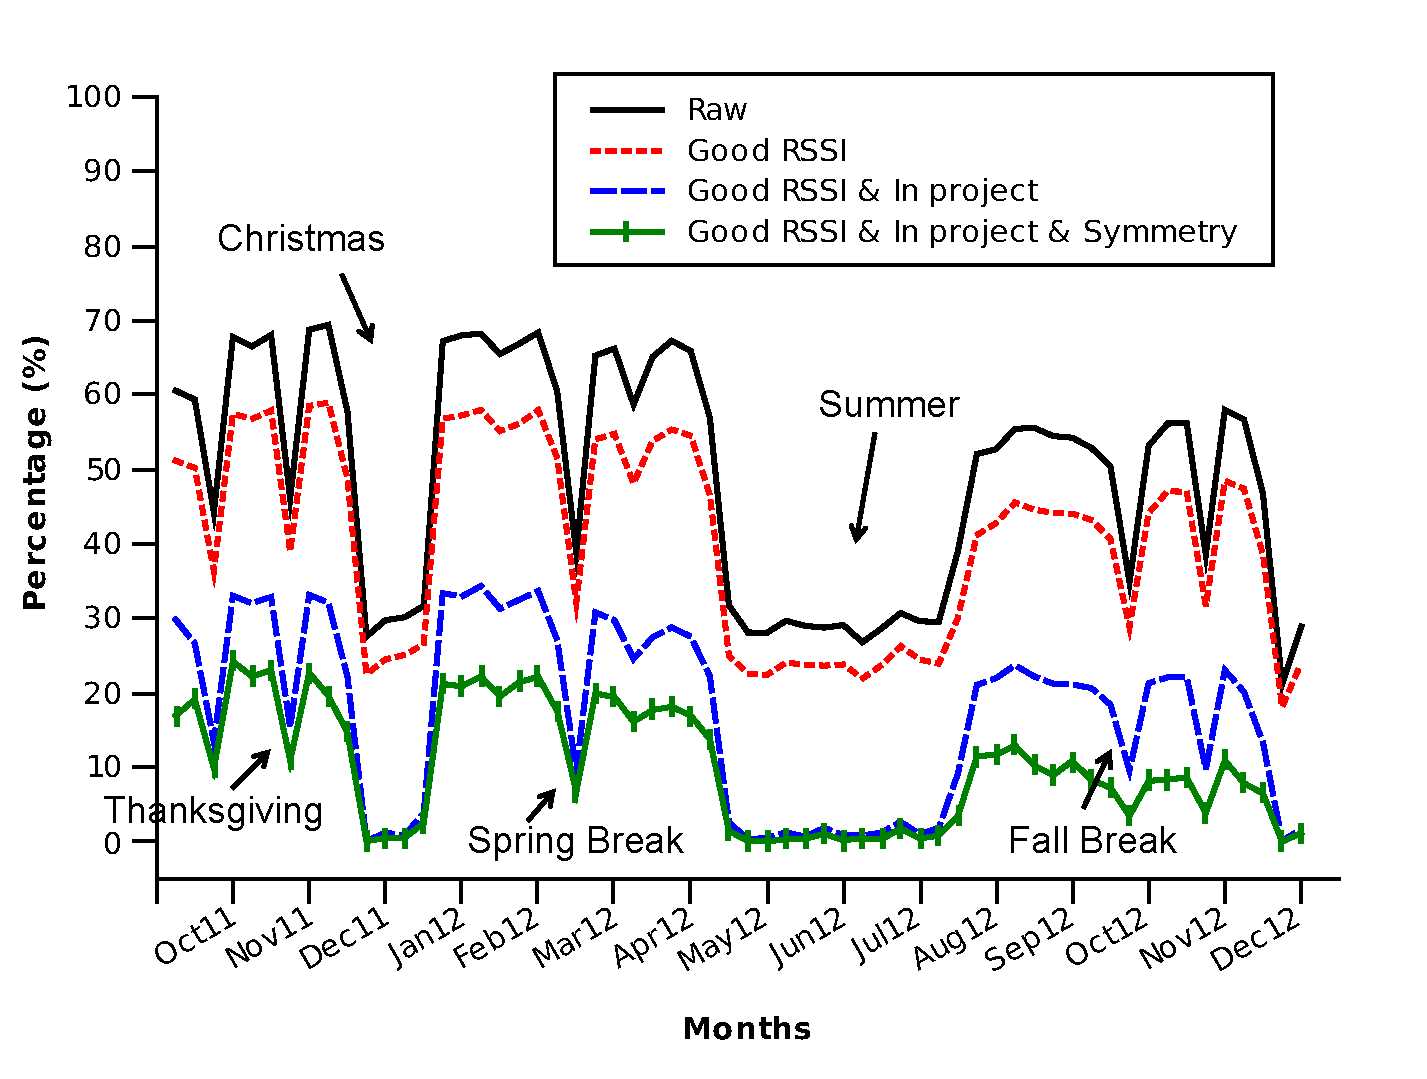
\includegraphics[width=3.5in]{graphs/weekly_bluetooth_with_symmetry_tag.pdf}}
\caption{Bluetooth Proximity with Different Restrictions} 
\label{fig:bluetooth}
\end{figure} 

Given that the students were selected from a core group of six dormitories, a natural skepticism should emerge from the data with regards to the diurnal effects of proximity, namely proximity does little good if it only occurs at night when the phone is not otherwise being used (ex. sleeping in the dorm room).  Hence, we analyze the diurnal distribution of Bluetooth proximity by dividing one day into three parts: day time (8am to 4pm), night time (4pm to 12am) and sleep (12am to 8am). In this way, we are able to investigate the impacts of time durations on such proximity. Figure~\ref{fig:diurnal} shows the diurnal distribution with the twin restrictions of good RSSI and intra-study detected proximity only. The daytime proximity percentage from 8am to 4pm is larger than the value during nighttime and almost equal to the value of sleep time.  The separation from in the fall of 2012 largely follows the classroom / major separation as noted in the raw and restricted graphs. 

\begin{figure}[tbp]
\centering 
{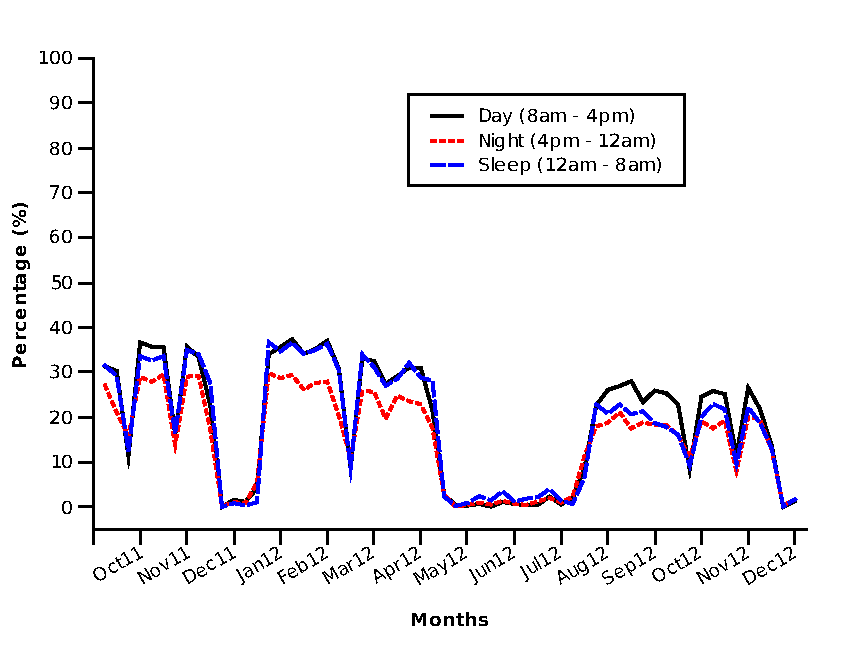
\includegraphics[width=3.5in]{graphs/weekly_bluetooth_diurnal.pdf}}
 \caption{Diurnal Distribution of Bluetooth Proximity} 
\label{fig:diurnal}
\end{figure} 

Beyond coarse diurnal metrics, significant day of week effects can also exist. Course patterns can vary dramatically between the Monday / Wednesday / Friday courses and Tuesday / Thursday courses.  Similarly, weekends are much more likely to be quite diverse from normal weekday patterns.  Figure~\ref{fig:diurnal_april} shows the daily Bluetooth proximity and diurnal distribution in April 2012 for a more detailed comparisons among the weekdays with each respective Saturday noted on the x axis. The peak values always appear at the beginning of the week and decrease slowly during the week. During the Easter holiday (April 6th - April 9th), the opportunities for proximity shrink dramatically as the students travel home for Easter break. Meanwhile, more Bluetooth proximity appeared in the later hours (broadly defined as sleep time) than daytime hours during weekend which indicates the participants spent more time in closer proximity to others during those time periods largely as a byproduct of social relationships. 

\begin{figure}[tbp]
\centering 
{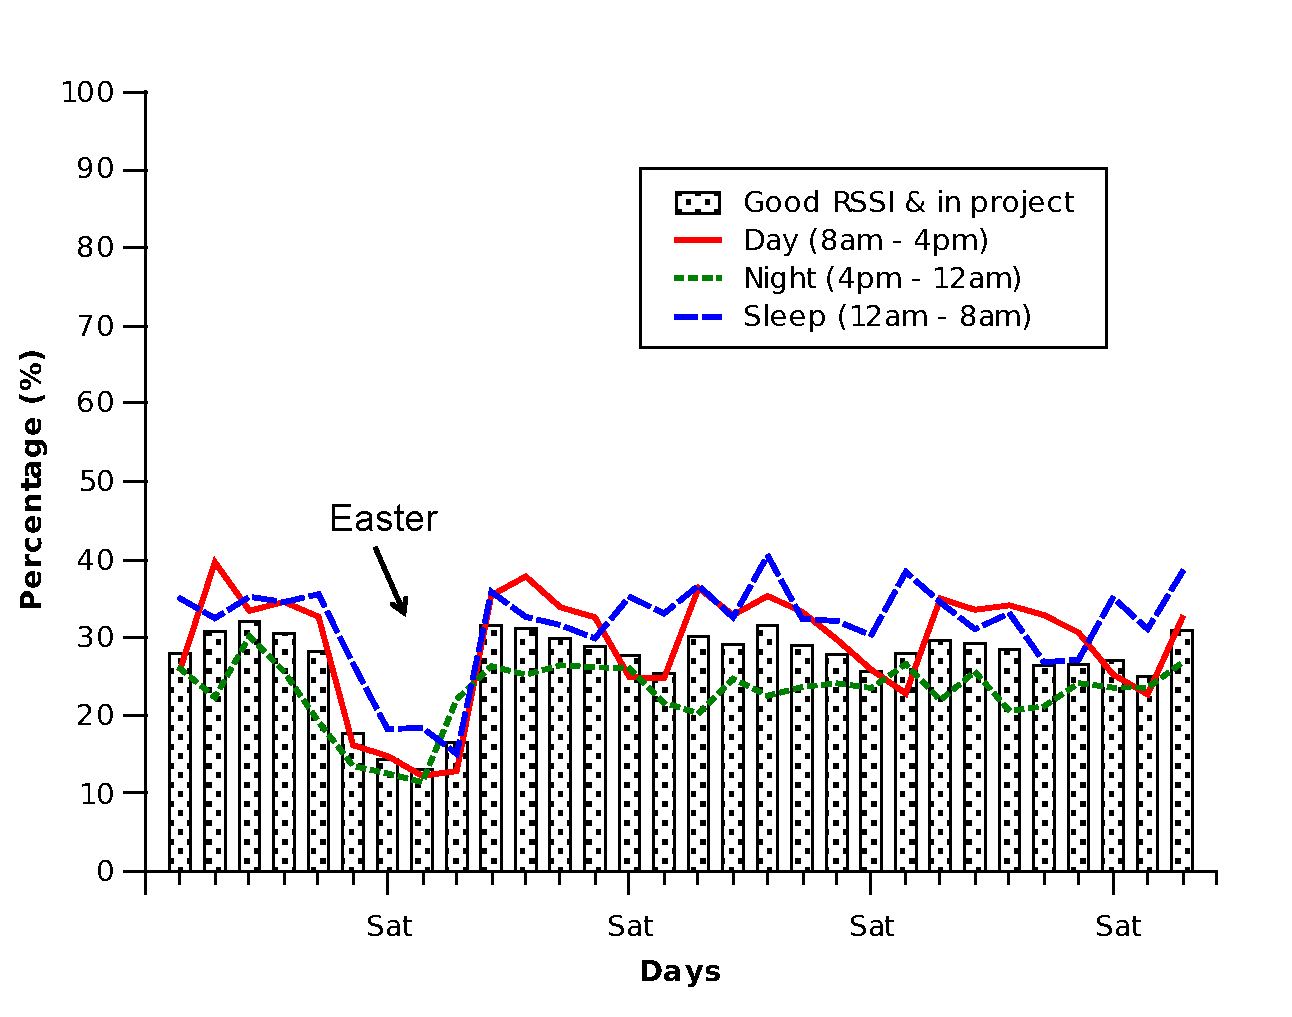
\includegraphics[width=3.5in]{graphs/bluetooth_201204_tag.pdf}}
\caption{Diurnal Distribution of Bluetooth Proximity in April 2012} 
\label{fig:diurnal_april}
\end{figure} 

For WiFi proximity, we analyze the number of time slots when the device shares at least two of the same access points with another device (in-study devices only) and we calculate the percentage of such time slots. Figure~\ref{fig:wifi} demonstrates the WiFi proximity and its diurnal distribution across the study period. During the holidays and summer, the percentage is almost zero as only university APs are considered for WiFi performance. Compared to other periods, WiFi proximity during daytime from 8am to 4pm represents a slight uptick though not statistically significant variation over other periods. 

\begin{figure}[tbp]
\centering 
{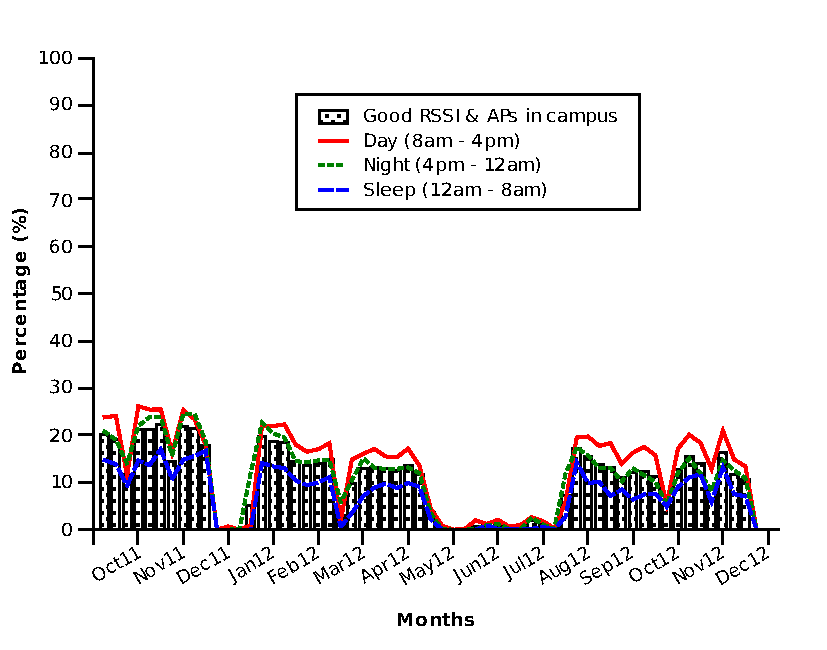
\includegraphics[width=3.5in]{graphs/weekly_wifi.pdf}}
\caption{WiFi Proximity} 
\label{fig:wifi}
\end{figure} 

Taking a bit more of an optimistic stance, we combine both WiFi proximity detection and Bluetooth proximity detection to create a combined proximity.  Note that earlier proximity measurements used either exclusively Bluetooth or WiFi.  Broadly defined, in one specific time slot, if the device can either detect other devices within the project with good Bluetooth RSSI or share at least two same APs in the campus with good WiFi RSSI, this time slot is counted as one of the slots when the device is in proximity with another device (intra-study only). Figure~\ref{fig:bt_wifi} illustrates such proximity across months. Compared to Bluetooth proximity only or WiFi proximity only, the percentage is increased to more than 40\% trailing to roughly 30\% by the end of the study, a nearly 10\% increase over Bluetooth only considerations. The diurnal distribution keeps the same trend and the proximity percentage during the daytime being is the highest among the respective time periods.

\begin{figure}[tbp]
\centering 
{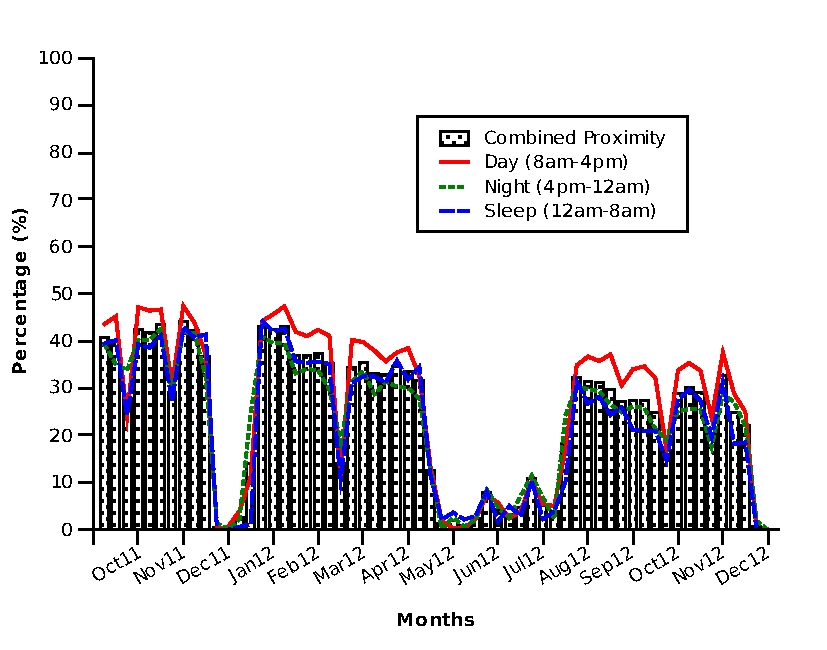
\includegraphics[width=3.5in]{graphs/weekly_bt_wifi.pdf}}
\caption{Combined Proximity (Fused Bluetooth / WiFi Detection)} 
\label{fig:bt_wifi}
\end{figure} 

\subsubsection{Intercontact Time and Beyond}
Intercontact time is defined as the time elapsed between two successive contact periods for a given pair of devices~\cite{chaintreau2007impact} and it is another important characteristic of prevalence. For each pair of devices, we compute the intercontact time as the time takes before the pair meet again. Figure~\ref{fig:intercontact_cdf} exhibits the empirical distribution of the intercontact times obtained among different months. On average, the intercontact time is around 1000 minutes which is more than 16 hours. The distribution varies only slightly with the earlier time periods (Nov 2011) exhibiting a shorter inter-contact time, in large part due to more shared coursework, reinforcing the findings from earlier graphs.  

\begin{figure}[tbp]
\centering 
{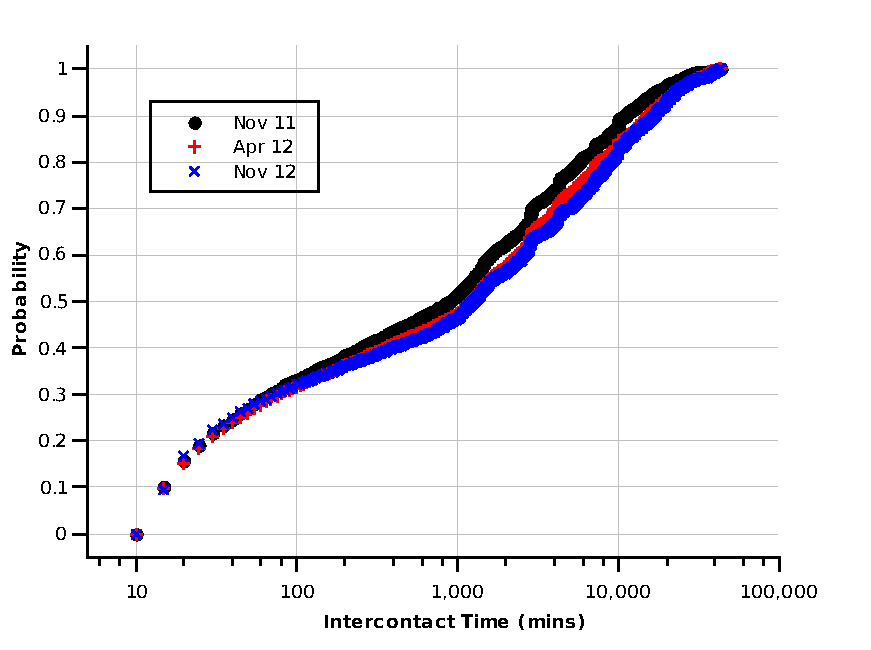
\includegraphics[width=3.5in]{graphs/intercontact_cdf.pdf}}
\caption{Intercontact Time ECDF} 
\label{fig:intercontact_cdf}
\end{figure}

\subsubsection{Measuring Effective Utility}
The final aspect for prevalence is the notion of effective utility, namely that the opportunity must occur when it is actually needed.  From a general perspective, that need can happen when the following two conditions are satisfied: a) the node $MN_i$ has some traffic to receive or send but no direct / poor connection is available  b) there is some other node $MN_j$ in proximity which can work together with the node. We analyze how often the devices really need relaying in the following three types of context. 

In order to find the appropriate range values for reasonable WiFi performance, we conducted experiments to evaluate the cutoff points of WiFi RSSI on the particular Android handset employed (Nexus S).  Channels were selected to be orthogonal to campus WiFi deployments (via a specially marked research channel space for our building) with distance, orientation, and other factors varied to get a wide variety of channel characteristics.  Downloads were conducted over 100 times for each particular configuration and the results explored for throughput.  Based on the experiment results of AP RSSI values and the corresponding throughputs, we note that -80 dBm can be the threshold to indicate good link quality with throughputs dramatically ramping up shortly after -80 dBm. At the same time, according to the RSSI distribution in Figure~\ref{fig:rssi}, there are more than 40\% of records showing that APs in campus having RSSI values larger than -80 dBm.  Therefore, we use -80 dBm as the good RSSI threshold to indicate good WiFi connection.  

The first context is when the device has traffic but does not have good WiFi connection. Figure~\ref{fig:traffic_80} includes two sets of results in Nov 2012: one is the percentage of having traffic and the other is the percentage of having traffic but the device does not have good WiFi connection (all the detected access points have signal strength less than -80dBm). Based on the results, there are more than 80\% of time slots have traffic while 30\% among them do not have good WiFi connection to do the transmission. Without WiFi, the traffic goes through the mobile link which further imposes pressure on mobile networks. However, relaying can work as an alternative to do the traffic offloading. 

\begin{figure}[tbp]
\centering 
{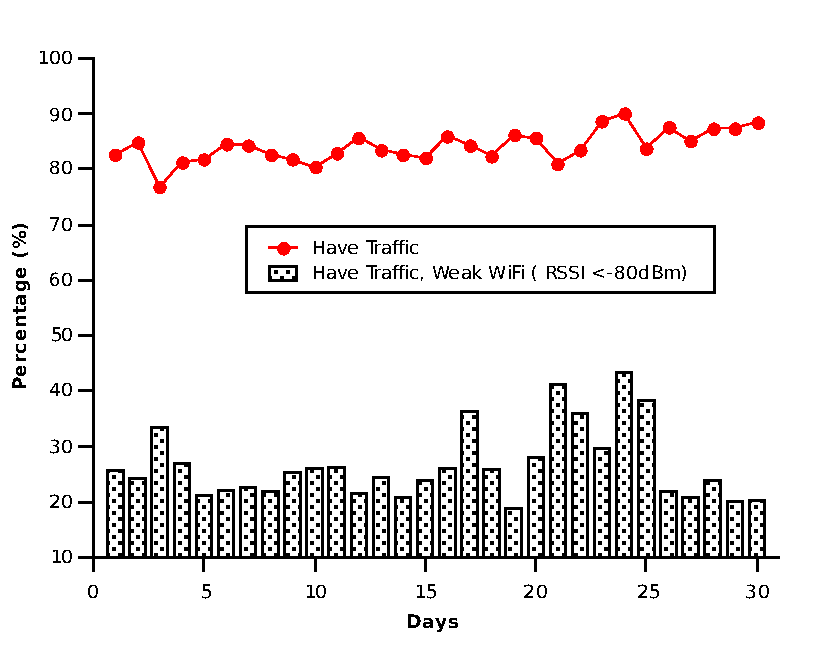
\includegraphics[width=3.5in]{graphs/traffic_80.pdf}}
\caption{Weak WiFi Signal \& Traffic} 
\label{fig:traffic_80}
\end{figure}

The second context is from the aspect of WiFi RSSI. With the prevalence of WiFi, it is interesting to investigate how often devices are not be fully covered by WiFi, i.e., detect no WiFi access points with RSSI larger than -80dBm. In such case, relay is an option. In Figure~\ref{fig:80_relay}, nearly 40\% of the time the devices do not in good WiFi environment on average. Among these time slots, there are around 20\% of them do have relaying node(s) around. 

\begin{figure}[tbp]
\centering 
{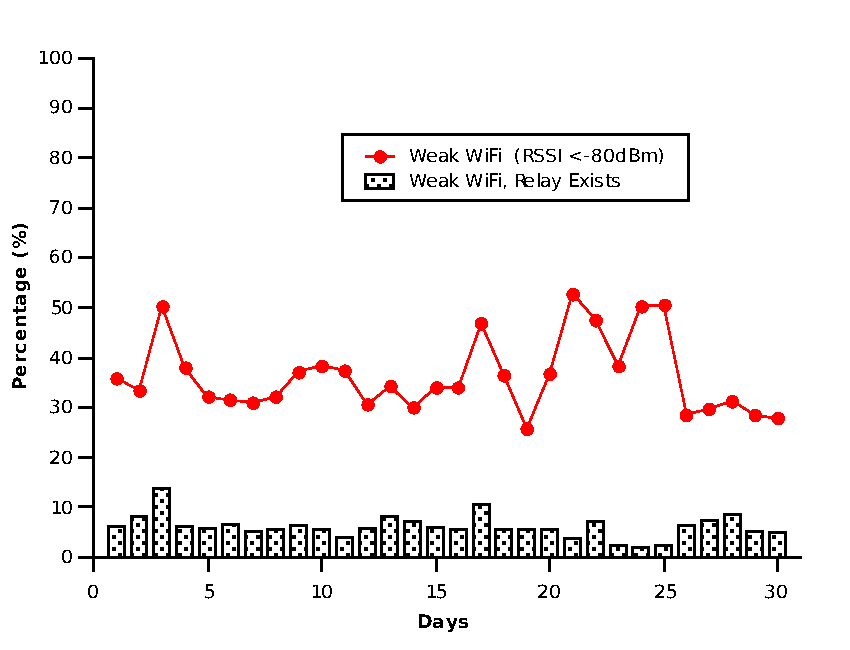
\includegraphics[width=3.5in]{graphs/80_relay.pdf}}
\caption{Relaying \& Weak WiFi Signal} 
\label{fig:80_relay}
\end{figure}

In the third context, we consider the further benefits which relaying may produce. Besides WiFi and mobile network, relaying provides the third option to transmit traffic. When there is traffic need, the device may use relaying even it has established WiFi connection. Such cases happen when the relaying nodes have the content the device requests or the relaying communication has better link quality. Based on the results shown in Figure~\ref{fig:relay_traffic}, the percentage is pretty high when relaying exists and there is traffic at the same time. Therefore, relaying can provide great opportunities for devices to send and receive traffic, not only in a passive way, but also in a proactive way. 

\begin{figure}[tbp]
\centering 
{\includegraphics[width=3.5in]{graphs/relay_traffic.pdf}}
\caption{Traffic \& Relaying} 
\label{fig:relay_traffic}
\end{figure}

\subsubsection{Evaluating Prevalence} 

To summarize, we conclude our explorations on prevalence with a brief discussion of metrics and conditions used to evaluate prevalence, i.e. the potential for opportunistic communications.  

\begin{itemize}
	\item Time in Proximity: It is the most important metric for prevalence and the premise for opportunistic communication. Without enough time in proximity, any relaying protocols cannot be deployed in practice. Through the analysis of data collected from nearly 200 smartphones in the campus environment, we demonstrate such prevalence is significant. 
	\item Intercontact time: As mentioned in the last section, intercontact time is the time duration between two continuous meets for a given pair of devices. It is another characterization to indicate the frequency with which data can be transferred between networked devices.  While relevant for approaches such as DTNs, intercontact time has less relevance for single hop relaying or collaborative opportunistic communications.  
	\item Effective Utility: The prevalence of opportunities offer little utility to the handset if said prevalence occurs when the device has or no data to send, i.e. those opportunities need to occur where and when you need them.  Effective utility measures the cases where traffic demand exists and appropriate conditions exist to deliver improved wireless performance.       
\end{itemize} 

\subsection{Stability}

Prevalence becomes of little use if the set of devices available for opportunistic communications are constantly in flux.  While traditional opportunistic networking approaches assume a degree of shared trust, there exists a non-zero cost for the establishment of secure point-to-point channels or at a minimum, the assurance that the device being considered for point-to-point communications is indeed legitimate.  To that end, we evaluate the data through the lens of \emph{stabilty}, namely to what extent are the devices available detected for communication likely to be available for a reasonable duration of time.  Hence, the primary measure of stability lies in the distribution of contact durations with considerations for sufficient signal strength and symmetric connectivity detection.  Put simply, candidates for opportunistic communications must exist for a reasonable duration of time on the order of minutes, not simply seconds to amortize the cost of point-to-point channel negotiation over the lifetime of the opportunity.       

In a complementary sense, trust between various devices can be realized not only through duration but also through the repeated appearances in the local proximity.  Although an individual node may have long inter-contact times individually, the fact that a node appears consistently at multiple times per day or multiple times per week for a reasonably stable period of time implies a likely social construct or external relationship between the devices.  Hence, a secondary metric for stability is the degree to which the most frequent nodes churn, i.e. are the extent to which nodes appear for opportunities uniformly distributed and infrequent or are there nodes that appear dramatically more often than other nodes, potentially allowing for extended trust to be constructed by virtue of repeat appearances (or at a minimum, the trust exchange accelerated due to prior exchanges).  

Hence, Figure~\ref{fig:duration} explores the most basic aspect of stability, namely the average duration of devices as present with regards to the locally detected nodes. Further filtering is applied where a node must have been seen at least once per day by that node for consideration for opportunistic communication. Critically, the average stability of a connection falls at roughly 6 minutes, a considerable time period for conducting the security negotiations at the front of the communication.  

\begin{figure}[tbp]
\centering 
{\includegraphics[width=3.5in]{graphs/duration_cdf_2.pdf}}
\caption{Proximity Duration ECDF} 
\label{fig:duration}
\end{figure}

Moreover, node strength is another metric used to evaluate the stability of proximity nodes and it is defined as follows: In one time slot, if the device detects a proximity device then the total appearance times of this peer is increased by one. Node strength is the total number of appearances of a proximity device in the period. Based on the data across 15 months, we get the node strength of proximity nodes for devices and analyze the relationship between number of relays and node strength in Figure~\ref{fig:node_strength_all}. Using the threshold of 500 for node strength, we remove those infrequent proximity nodes and calculate the average node strength for each device. It is interesting that most of the nodes have less than 10 frequent proximity nodes (loosely correlating with their social circles) and the corresponding average node strength is relatively higher than those with more than 10 frequent relays. 

\begin{figure}[tbp]
\centering 
{\includegraphics[width=3.5in]{graphs/node_strength_all_tag.pdf}}
\caption{Number of Proximity Nodes vs. Node Strength } 
\label{fig:node_strength_all}
\end{figure}

While node strength captures the raw magnitude of total time spent together and indirectly infers longitudinal behavior, Figure~\ref{fig:total_continuous_cdf} takes the concept further by examining the `streakiness' over multiple days by which a potential peer is likely to appear across the entire duration of the study. The total appearances represents the distribution of how frequently a node is likely to appear whereby if the prospective peer is seen at least once in the day, it counts as being successfully seen for the purposes of consistency. Note that for the purposes of the graph, all nodes are considered rather than only the nodes with a reasonable degree of consistency to capture the full longitudinal nature of the study. No filtering is done either for sufficiency of signal strength. Interestingly, several nodes eclipse nearly two-thirds of the time in the study in terms of consistency of meeting.  It is those nodes that appear consistently that represent the stable foundation from which the prevalence can be effectively leveraged.
The other plot in the graph captures the distribution of continuous days, namely if a node appears more than one day in a row, how long is the streak likely to continue with subsequent appearances over the next few days? The average number of continuous days is 1 day which means over 50\% of the proximities did not happen continuously by day.    

\begin{figure}[tbp]
\centering 
{\includegraphics[width=3.5in]{graphs/total_continuous_cdf.pdf}}
\caption{Total Appearances and Continuous Appearances in Day Counts ECDF}
\label{fig:total_continuous_cdf}
\end{figure}

From the perspective of number of proximity devices, we calculate the cumulative number and compare it with the indeed active number to analyze the stability of prospective relays. The cumulative number is defined as the total number of distinguished relays in history while the weekly active number is the total number of relays which appear in the current week and were active in the past one month. Figure~\ref{fig:cumulative_active} illustrates the weekly cumulative number and active number across 15 months. The cumulative number increases to a limit (nearly the total number of devices within the project) and such value is quite stable in the following months. Meanwhile, the active number decreases across the study and big decreases happen when semesters change.  

\begin{figure}[tbp]
\centering 
{\includegraphics[width=3.5in]{graphs/cumulative_active.pdf}}
\caption{Weekly Cumulative Number and Active Number} 
\label{fig:cumulative_active}
\end{figure} 

Therefore, there are four important points for the evaluation of stability:

\begin{itemize}

\item Duration: The duration of relaying connection is essential for successful traffic transmission between the device and its relaying nodes. If two devices come across each other and separate soon, such proximity is not suitable for the establishment of usable connection. We roughly define a mean average of duration as needing to be an order of magnitude or better versus trust establishment for the mobile-to-mobile link.

\item Node Strength: The usage of node strength can capture the degree to which a trusted subset of mobile peers emerge that have the potential for expedited trust for opportunistic efforts (i.e. negotiate heavy once, light weight for the next $N$ times).

\item Total Appearances: While a purely opportunistic network where a de facto sense of trust exists can tolerate frequent dynamics in terms of random nodes serving as relay or collaboration partners, consistency of the peering partner for a node can both elicit trust by virtue of familiarity (repetition) which also has roots in normative social structures. 

\item Continuous Appearances: Although trust can be more easily inferred by virtue of repetition, consistent trust over continuous days likely implies a stronger degree of trust (not a guarantee, simply more likely). The continuous consistency ($\geq 1 /$day, $\geq 1 / $ week) can serve as a complementary metric to the earlier aforementioned inter-contact time espoused in traditional opportunistic network evaluations.
\end{itemize}

\subsection{Reciprocity}

Finally, a key metric for evaluating the potential opportunistic communication is the degree to which reciprocity exists, ideally converging to an equal ratio of service versus need.  Although altruism amongst nodes typically leads to a healthier network performance as a whole, the potential for increased energy consumption is of little consolation if the device is always helping but never benefitting.  To that end, we posit that reciprocity amongst nodes must be taken into account when considering the overall utility of an opportunistic solution.  Whereas much of the prior work is limited to evaluating only some aspects of prevalence and stability, interactions among pairs (dyads) in the study afford us the ability to evaluate the extent to which reciprocity exists both in short and long-term time scales with actual traffic patterns and actual energy constraints.  

To that end, Figure~\ref{fig:reciprocal} shows the daily average percentages with respect to needing assistance (relaying to another node) versus offering assistance (relaying for another node).  The data is drawn strictly from intra-study interactions across the month of November 2012.  A mobile node is defined as needing assistance if it has traffic but detects no WiFi access points with a sufficient signal strength ($> -80 dBm$).  A mobile node is defined as serving (offering assistance) if it has a good WiFi connection and has been detected by other nodes within the study.  Hence, a value of 25\% with respect to being detected as a relay denotes that another node ($MN_j$) in the study detected the node ($MN_i$), $MN_j$ had a good signal strength to the node $MN_i$, and $MN_i$ had a good signal strength for WiFi for 25\% of the time that $MN_i$ was on for that day.  Critically, a node needing relaying but detecting no nodes is similar to a node being willing to serve but yet no nodes needing its service. A further sub-division is done to breakdown the nodes filtered if battery level were taken into consideration, i.e. what percentage could no longer offer assistance if the battery level fell below 30\% which barely has an impact, typically only a reduction of 1-3\% for the number of times a node could offer assistance but would not due to energy constraints.   

\begin{figure}[tbp]
\centering 
{\includegraphics[width=3.5in]{graphs/reciprocal.pdf}}
\caption{Distribution of Potential Interactions - Need vs. Serve (November 2012)} 
\label{fig:reciprocal}
\end{figure} 

For a reasonable portion of the time, most nodes on average have an increased need for assistance versus the ability to serve.  The primary exceptions emerge on weekends which also happen to correspond with football games, campus events, and travel.  
Figure~\ref{fig:1117} captures this relationship on both short-term (single day) and longer-term (one week/one month) timescales drawing from a single week from Figure \ref{fig:reciprocal}.  The figure plots the distribution of the node having the potential to serve versus needing assistance.  A ratio of one implies that the node had an equal number of time slots where the node could serve as a relay (detected, good WiFi) versus the node needing a relay.   Whereas the traffic from the weekend shows much stronger need (due in part to the lack of WiFi at the football stadium), the nodes on the long-term scale have ratios much closer to 1 representing a reasonable reciprocity.  Moreover, the typical weekday (as opposed to the game day scenario with limited WiFi) gravitates more closely to a balanced distribution as well.  Similarly as diurnal analysis in Section~\ref{sec:prevalence}, the diurnal distribution of such ratio is shown in Figure~\ref{fig:diurnal_ratio}. Notably, the ratio is most balanced in daytime while the needing is more than offering due to the lack of WiFi during the night and sleep time. 

\begin{figure}[tbp]
\centering 
{\includegraphics[width=3.5in]{graphs/1117_2.pdf}}
\caption{Ratio of Needing vs. Serving (November 2012)} 
\label{fig:1117}
\end{figure} 

\begin{figure}[tbp]
\centering 
{\includegraphics[width=3.5in]{graphs/diurnal_ratio.pdf}}
\caption{Diurnal Distribution of Ratio (November 2012)} 
\label{fig:diurnal_ratio}
\end{figure} 

To close, we list the essential criteria related to reciprocity and their formal definitions as follows:

\begin{itemize}

\item Needs Service: A critical first step to establishing the likely reciprocity is to characterize the share of time that a node is in the need service state, namely does the node either have poor / none WiFi or alternatively poor / no cellular coverage. The need service case is where the node will perceive value to the underlying opportunistic communications.

\item Offers Assistance: In contrast to needing service, the ability to offer service represents the altruistic aspects of needing service, namely when can the node assist other nodes? The share of when a node can offer relaying / collaboration must be considered along with energy filters excluding devices with low energy levels.

\item Service vs. Assistance: The final and most critical component is the actual ratio of reciprocity itself, ex. how often is the device likely to serve versus the device need service? While atypical situations can exacerbate sharing (everyone needs help), the normative situation should be one where reciprocity is preserved both on short-term timescales (daily) and long-term timescales (weekly, monthly).

\end{itemize}

\section{Summary}

Critically, we investigate the availability of opportunity for relaying and demonstrate that not only is such opportunity more prevalent than expected, the opportunities are stable enough to be worthwhile to establish even with auxiliary security constraints and the opportunities are reciprocal across both short-term and long-term time scales even when considering energy levels of the involved devices. Specifically, the key contributions are as follows:

\begin{itemize}
	\item \emph{Investigate the availability of opportunity for relay:} Proximity among mobile devices is the key to determine whether relaying can happen or not. Based on  Bluetooth and WiFi detections, we are able to use appropriate signal strength to reflect the relative distance of devices. Moreover, power is essential for mobile devices therefore residual battery is another important fact to be considered for availability.
	 
	\item \emph{Demonstrate the opportunity (prevalence) for relaying is indeed significant:} Through the analysis of a 15 month dataset of detailed smartphone data gleaned from nearly 200 smart phone users, we demonstrate that a typical user can find devices amenable to relaying averaging nearly 60\% of the time. To the best of our knowledge, we believe our study is the first to conduct a longitudinal study of relaying prevalence with demonstrating ample opportunities with respect to both raw relaying prevalence and useful relaying prevalence .  

	\item \emph{Demonstrate that said opportunities for relaying are not only prevalent but stable:} We show with our study data that relaying opportunities existing on average for durations of 6+ minutes. Moreover, we show that the opportunities for relaying tend to be highly focused on a select subset of devices enabling enhanced levels of trust versus random, intermittent opportunities as espoused in the literature.  

	\item \emph{Demonstrate that said opportunities would largely be reciprocal:} In addition to opportunities being prevalent and stable (useful), we show that interactions for relaying would be overwhelmingly reciprocal in both short-term and long-term time windows, even when accounting for the energy levels of both parties involved in the relaying.  We demonstrate this through the inclusion of actual traffic demands on fine temporal granularities, a unique feature of our dataset.  

	\item \emph{Propose a framework to evaluate the relaying potential for network traces:} While we believe our work is one of the first of its kind to fuse fine-grained proximity and traffic data over such a long period, we hope that others will embark on similar efforts to broaden the effective data pool available to the community.  To that end, we view all of our data through the lens of what we dub the APSR (Availability, Prevalence, Stability, Reciprocity) framework, a framework for systematically evaluating the potential and quality of the proximity of mobile network trace data.  
\end{itemize}




%
% Chapter 6
%

\chapter{Energy Consumption}
\label{chap:energy}



%
% Appendix
%

\appendix

%
% Modified by Sameer Vijay
% Last Change: Wed Jul 27 2005 13:00 CEST
%
%%%%%%%%%%%%%%%%%%%%%%%%%%%%%%%%%%%%%%%%%%%%%%%%%%%%%%%%%%%%%%%%%%%%%%%%
%
% Sample Notre Dame Thesis/Dissertation
% Using Donald Peterson's ndthesis classfile
%
% Written by Jeff Squyres and Don Peterson
%
% Provided by the Information Technology Committee of
%   the Graduate Student Union
%   http://www.gsu.nd.edu/
%
% Nothing in this document is serious except the format.  :-)
%
% If you have any suggestions, comments, questions, please send e-mail
% to: ndthesis@gsu.nd.edu
%
%%%%%%%%%%%%%%%%%%%%%%%%%%%%%%%%%%%%%%%%%%%%%%%%%%%%%%%%%%%%%%%%%%%%%%%%

%%%%%%%%%%%%%%%%%%%%%%%%%%%%%%%%%%%%%%%%%%%%%%%%%%%%%%%%%%%%%%%%%%%%%%%%
%
% Appendix
%
%%%%%%%%%%%%%%%%%%%%%%%%%%%%%%%%%%%%%%%%%%%%%%%%%%%%%%%%%%%%%%%%%%%%%%%%

\begin{table}[ht] 
\caption{Detailed Information of Collected Data } 
\centering  
\begin{tabular}{c|l|l}
\hline
		  Type			& Collected Information 					& Frequency \\ [0.5ex] 
\hline\hline Location			& Provider/Latitude/Longitude/Accuracy		& 10 min/100 meters	\\ 
\hline	  Bluetooth 		& ID/MAC/RSSI	    						& 1 min \\
\hline 	  WiFi 			& AP name/MAC/RSSI					& 3 min \\
\hline 	  Cell   			& 									& when RSSI changes \\
\hline	  Battery			& Charge method/Level	    				& when level changes at least 1 \\
\hline	  Light			& Level	    							& when level changes at least 30 \\
\hline	  Screen			& On/Off 							 	& when screen on/off \\
\hline 	  Camera			& Picture/Video name			        	        & when created	 \\
\hline 	  Network Traffic 	& Type/Cumulative bytes					& 1 min	 \\
\hline	  App Traffic		& Type/Name/Cumulative bytes			& 1 min \\
\hline	  App Status 		& Name/Permission/Total number			& 1 day \\
\hline 	  Port Traffic	        & Protocal/State/Pid/Src/Dst/Name			& 15 min \\
\hline 	  Password	  	& Type/Encrypted pwd/Salt				& 1 hour \\
\hline 	  Contacts			& Phone number/Email/Total number		& 1 day \\
\hline 	  Connection		& Status								& when status changes \\
\hline 	  Storage			& Total vol/Free vol						& 12 hours \\
\hline 	  Version			& Version number							& when phone starts \\
\hline 	  Phone Call		& Number/Duration						& 1 hour \\
\hline 	  SMS			& Number/Length						& 1 hour \\
\hline 	  MMS			& Number/Type						& 1 hour \\
\hline 	  Mail			& Sender/Receiver/						& 6 min \\
\hline 	  Music			& Album name/Display name/Size			& 3 min \\
\hline 	  Browser History	& Title/Url/Visited Times					& 1 hour \\
\hline
\end{tabular}
\label{table:detailed_data} 
\end{table}



%
% Back stuff
%

% % comment out the following three lines
% if using chapter-wise bibliography

 \backmatter
 \bibliographystyle{nddiss2e}
 \bibliography{dissertation}

\end{document}

% End of ``example.tex''
